%
%
%
%%%%%%%%%%%%%%%%%%%%%%%%%%%%%%%%%%%%%%%%%%%%%%%%%%%%%%%%%%%%%%%%%%%%%%%%
\chapter{Stator-Rotor Interaction in a Transonic Turbine Stage}
\label{rt27.chap}
\heada{Transonic Turbine Stage}
\setcounter{footnote}{0}
%%%%%%%%%%%%%%%%%%%%%%%%%%%%%%%%%%%%%%%%%%%%%%%%%%%%%%%%%%%%%%%%%%%%%%%%
%
%
%
 This chapter presents a detailed  numerical analysis of a stator-rotor
 interaction in a typical high pressure (HP) turbine stage of contemporary
 turbomachines using both linear and non linear unsteady flow representations.
 The sources of unsteadiness on the rotor passage are evaluated
 from the steady-state outlet stator solution.
 These disturbances are Fourier transformed and split into
 vortical and potential components in order to assess the
 influence of each on the rotor unsteady aerodynamics.
 The computed results are compared with the experimental data
 measured at the Osney Laboratory's rotating turbine facility.
 Good qualitative, and in most cases quantitative, agreement has
 been obtained.
 In the final part of the chapter, the results of the linearised
 method are compared with those obtained from a non-linear time
 marching technique. There is a surprising overall agreement,
 which indicates that the unsteady flow field generated by
 relative blade motion
 can be considered a quasi linear phenomenon for the HP turbine
 studied.
%
%
%
%
%
%
%
\section{Introduction}
\label{intro_nonlinear.sec}
\headb{Nonlinear Navier-Stokes solver}{Introduction}
%
 Over the last decade, significant advances have been made
 in the area of turbulent-viscous simulations using unstructured
 grids.
 However, compared with their structured counterparts,
 standard unstructured grid solvers have lower computational
 efficiency in terms of speed and storage.
 Unstructured grids often use tetrahedral elements only,
 an approach which often leads to numerical problems when the region to be
 discretised has a preferred direction such as the boundary layer for a
 high-Reynolds number flow. However, there are no fundamental difficulties in 
 extending tetrahedral meshes to include further element types such as triangular prisms, 
 pentahedra and hexahedra.  
 Although both the discretisation of the computational domain and the flow solver
 will become more complex,  such a mixed-element approach will offer
 a better, more efficient approximation than using tetrahedral elements only.
 For instance, hexahedral elements will handle boundary layer flows much better
 than tetrahedral elements because they can be made very slender without
 creating excessively small internal angles. 
 In order to handle mixed-element meshes, the spatial discretisation
 of the governing equations needs to be formulated in such a way
 that the numerical algorithms can be applied in a uniform way to all
 element types.
 A relatively simple way of achieving such consistent numerical treatment
 is to employ an edge-based data structure, which can be obtained
 from either a finite volume (FV) or a finite element (FE) formulation
 if the mesh consists of tetrehedral elements only. In this particular case, 
 all nodes are connected directly without any internal diagonals.
 However, quadrilaterals in 2D and hexahedrals in 3D have not only
 edges but also diagonal links. Therefore, to create an edge-based
 data structure from mixed meshes, one cannot use a FE technique
 because of the non-zero shape function contributions from the
 diagonally-opposed nodes for which there are no direct edges.
 Consequently, we will use a FV technique to obtain an edge-based
 data structure from mixed element meshes but, as reported by
 Barth \citeyear{Barth:4}, Parthasarathy et al. \citeyear{Kallinderis:2},
 Mavriplis \& Venkatakrishnan \citeyear{Mavriplis:3}
 for unstructured meshes of tetrahedra, 
 the discretisation of the viscous terms, remains a major problem. 
 The FV edge-based data structure is usually obtained by
 discretising the viscous terms in two sequential  loops, the so-called
 two-loop approach. The first loop is used to construct the gradients
 at all points, and the second one forms the second derivatives from
 the computed gradient information.
 Using such a technique, 
 the viscous fluxes are treated in an analogous manner to
 the inviscid ones and no extra storage is required.
 However, this strategy, used by several authors
 (see Peraire et al. \citeyearNP{Peiro:2}, Vahdati \& Imregun \citeyearNP{Mehdi:3})
 has at least three serious drawbacks.
 First, the {\em odd-even decoupling} can destabilize
 the numerical scheme in regions where the viscous effects are
 important, e.g. the boundary layer.
 Second, for a 1D mesh of spacing $h$, the scheme will reduce to a second
 difference on a stencil of $2h$, a feature which will lower numerical
 accuracy.  Since packing enough points into the viscous layer
 is one of the main difficulties associated with viscous flow
 computations, a scheme that operates on every other point is highly
 undesirable.
 The third problem is the difficulty of implementing a viscous Jacobian which
 becomes important if an implicit time integration scheme is employed.

 An alternative approach, based on Galerkin
 finite element (GFE) approximation where velocity
 and temperature are made dependent variables,  is the derivation of the six node-pair
 coefficients for the Hessian matrix (Mavriplis \citeyearNP{Mavriplis:4},
 Selmin \& Formaggia \citeyearNP{Formaggia}).
 Each coefficient  is associated with  two nodes only, hence the term "node-pair GFE". 
 As mentioned earlier, such a formulation is not edge-based for non-tetrehedral meshes because 
 of the possible diagonal links between the nodes of a hexahedral element.
 On the other hand, the final discrete viscous
 terms of such a GFE formulation form a nearest neighbour stencil.
 Therefore, using the  Hessian node-pair
 coefficients, six second derivatives can be calculated for each node.
 Since the viscous terms can be expressed as a summation of the product
 of the node-pair coefficients and the unknowns,
 the construction of a viscous Jacobian becomes straightforward by explicit
 differentiation. Furthermore, the odd-even decoupling is avoided and the accuracy is improved.
 Unfortunately, this approach needs additional storage for the six node-pair
 coefficients and its applicability is restricted to triangular/tetrahedral
 elements if an edge-based data structure needs be employed.

 In summary, when dealing with mixed-element meshes, FV formulations can
 yield edge-based data structures but viscous flux discretisation
 remains problematic. On the other hand, GFE formulations are more
 efficient but the edge-based data structure cannot be preserved for non tetrahedral elements.  
 Therefore, the discretisation of the viscous fluxes
 can be improved by combining  the
 storage efficiency of the two-loop FV approach  with the
 numerical efficiency of the node-pair GFE method in an edge-based FV framework.

%
%
%
%
%
\section{Steady State Flow Analysis}
\label{rt27_steady.sec}
\headb{Transonic Turbine Stage}{Steady state flow}
%
%
 The analysis of the steady-state flow-field for
 the coupled NGV-rotor configuration is presented in this section.
 The flow is assumed to be fully turbulent
 and the high Reynolds number version of the Spallart-Allmaras
 \citeyear{Spalart:1} turbulence model
 is used together with a slip boundary condition on the solid walls. The
 wall shear stresses are evaluated using a generalized law of the wall
 as the one reported by White \citeyear{White:1}.
 Apart from predicting midspan pressure more accurately,
 3D calculations provide us with hub to tip
 distribution of the dependent variables
 and take the tip losses into account.
 When the air is turned through a row of axial blades,
 the flow far from the end walls,
 hub or casing, may often be considered as 2D.
 However near the end walls, the inlet boundary layer flow contains
 span-wise velocity gradients, and transverse velocities
 are produced once it is turned.
 The 2D flow is termed the {\em primary} flow
 and the 3D effects near the end walls are called {\em secondary}
 flows.
 Furthermore a turbomachinery rotor blade must have a small but finite clearance
 relative to its surrounding casing. The clearance, as in the case of rotor RT27a,
 is typically $1\%$ of the blade's span. However, the flow which leaks through
 this small gap has a surprisingly large effect on the aerodynamics of the machine
 especially when the blade is relatively short.
 In order to predict secondary flow effects and to take into account
 tip-leakages, the hub and tip sections must be treated as solid walls
 and a tip clearance must be included in the computational mesh.
%
%
%
\subsection{Computational mesh}
\label{rt27_mesh.subsec}
%
\begin{figure}
~\vspace{-30mm}\\
 \begin{center}
  \begin{tabular}{c}
    \subfigure[3D view]
       {\centerline{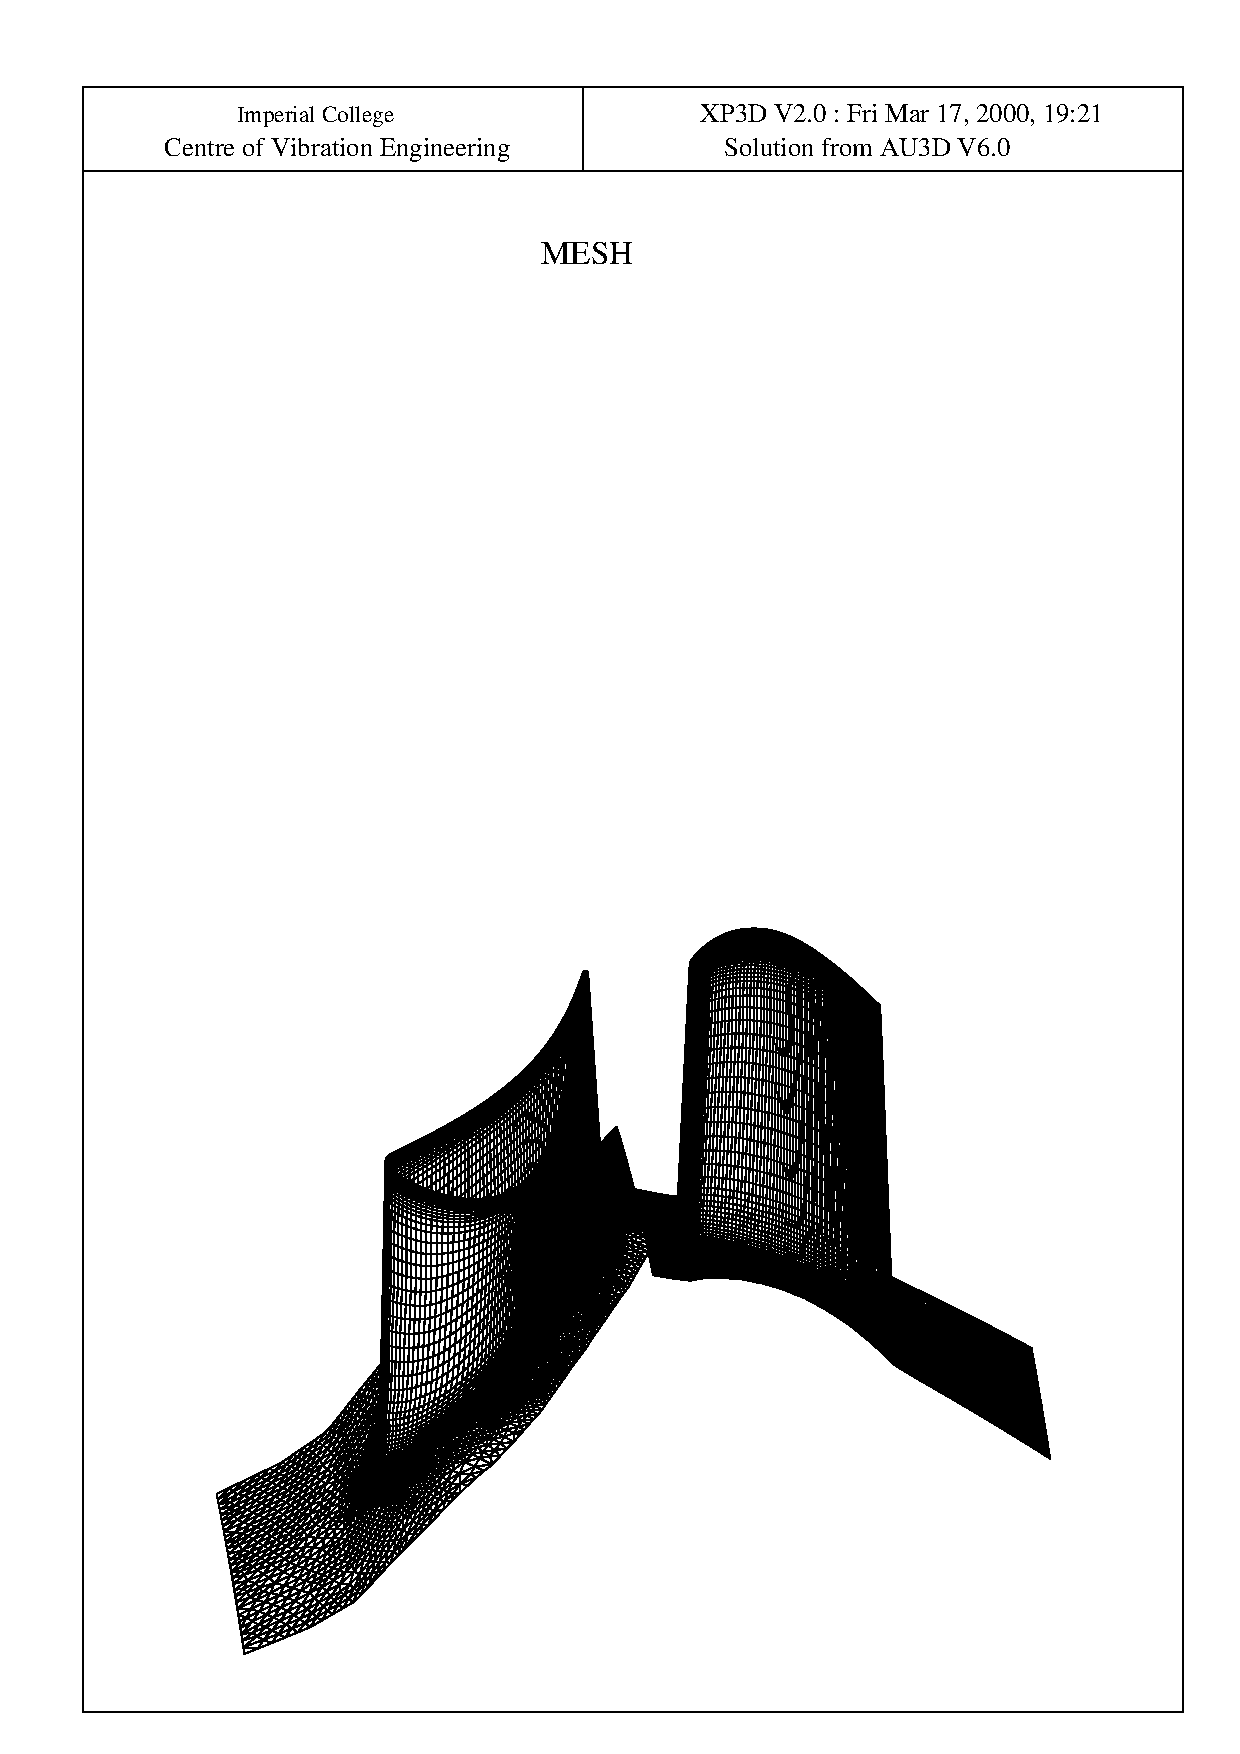
\includegraphics[width=140mm,clip=t]{CHAP_RT27/FIGURE/mesh3d_1.pdf}}}
        \vspace{-5mm}\\
    \subfigure[Meridional view]
       {\centerline{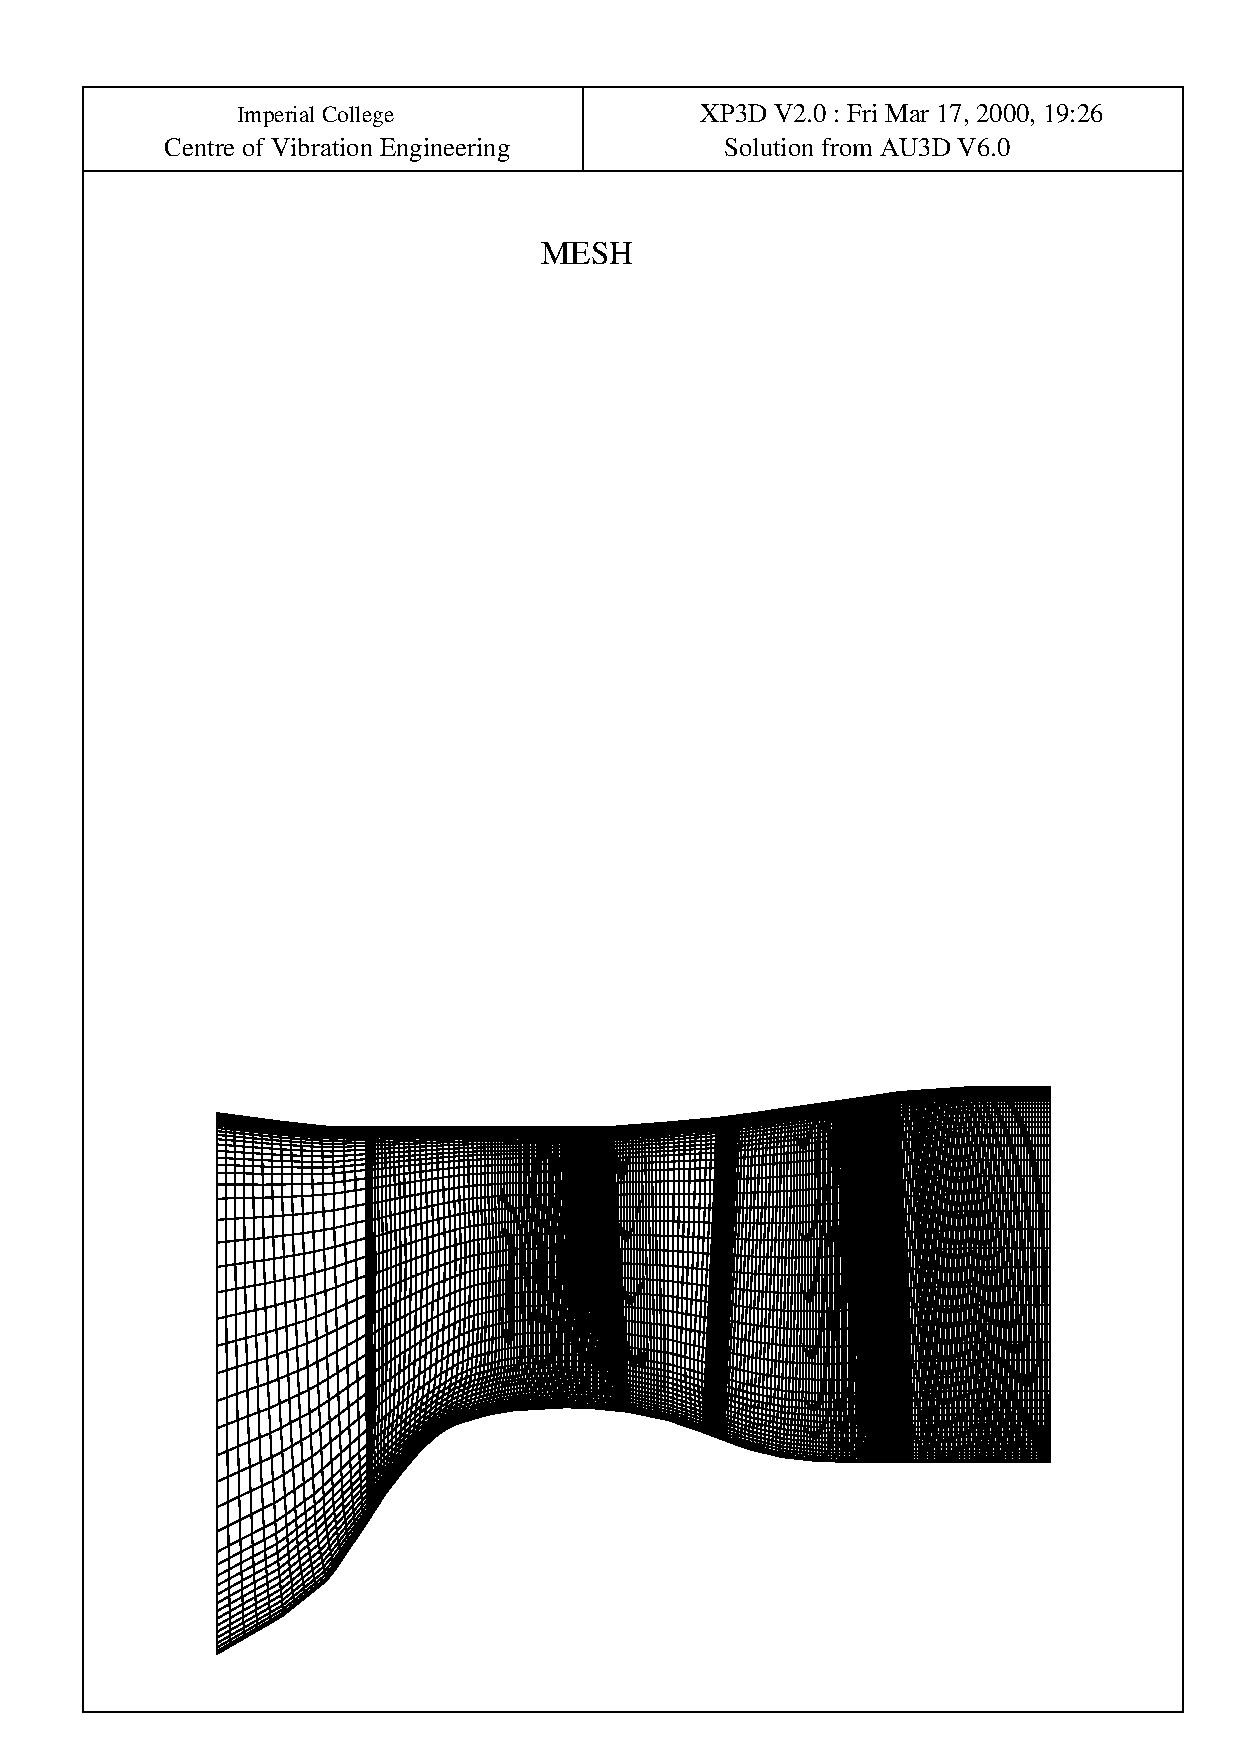
\includegraphics[width=140mm,clip=t]{CHAP_RT27/FIGURE/mesh3d_3.pdf}}}
  \end{tabular}
 \end{center}
 \vspace{-8mm}
 \caption{Computational mesh of RT27a turbine stage (564,660 points)}
 \label{rt27_mesh1.fig}
\end{figure}
%
 The computational meshes for the NGV and rotor passages were generated
 independently using the LEVMAP mesh generator described in chapter \ref{mesh.chap}.
 These two meshes were then assembled together for a coupled
 NGV-rotor steady-state calculation.
 The NGV outflow and rotor inflow are treated
 as two separate boundaries and they are responsible for the interaction
 between the two domains via a mixing layer process (Dawes \citeyearNP{Dawes:4},
 Denton \citeyearNP{Denton:1}).
 A 3D view of the grid is shown in Fig. \ref{rt27_mesh1.fig}a
 while Fig. \ref{rt27_mesh1.fig}b shows
 a meridional view of the blade surfaces together with one periodic boundary.
 The points in the radial direction are clustered towards the end walls
 because of the strong secondary flow expected in these regions. Also,
 additional grid radial-levels are used in the rotor tip-gap region
 to capture the tip leakage effects.
%
\begin{figure}[ht]
 \begin{center}
  \begin{tabular}{cc}
    \subfigure[Tip-gap radial mesh]
       {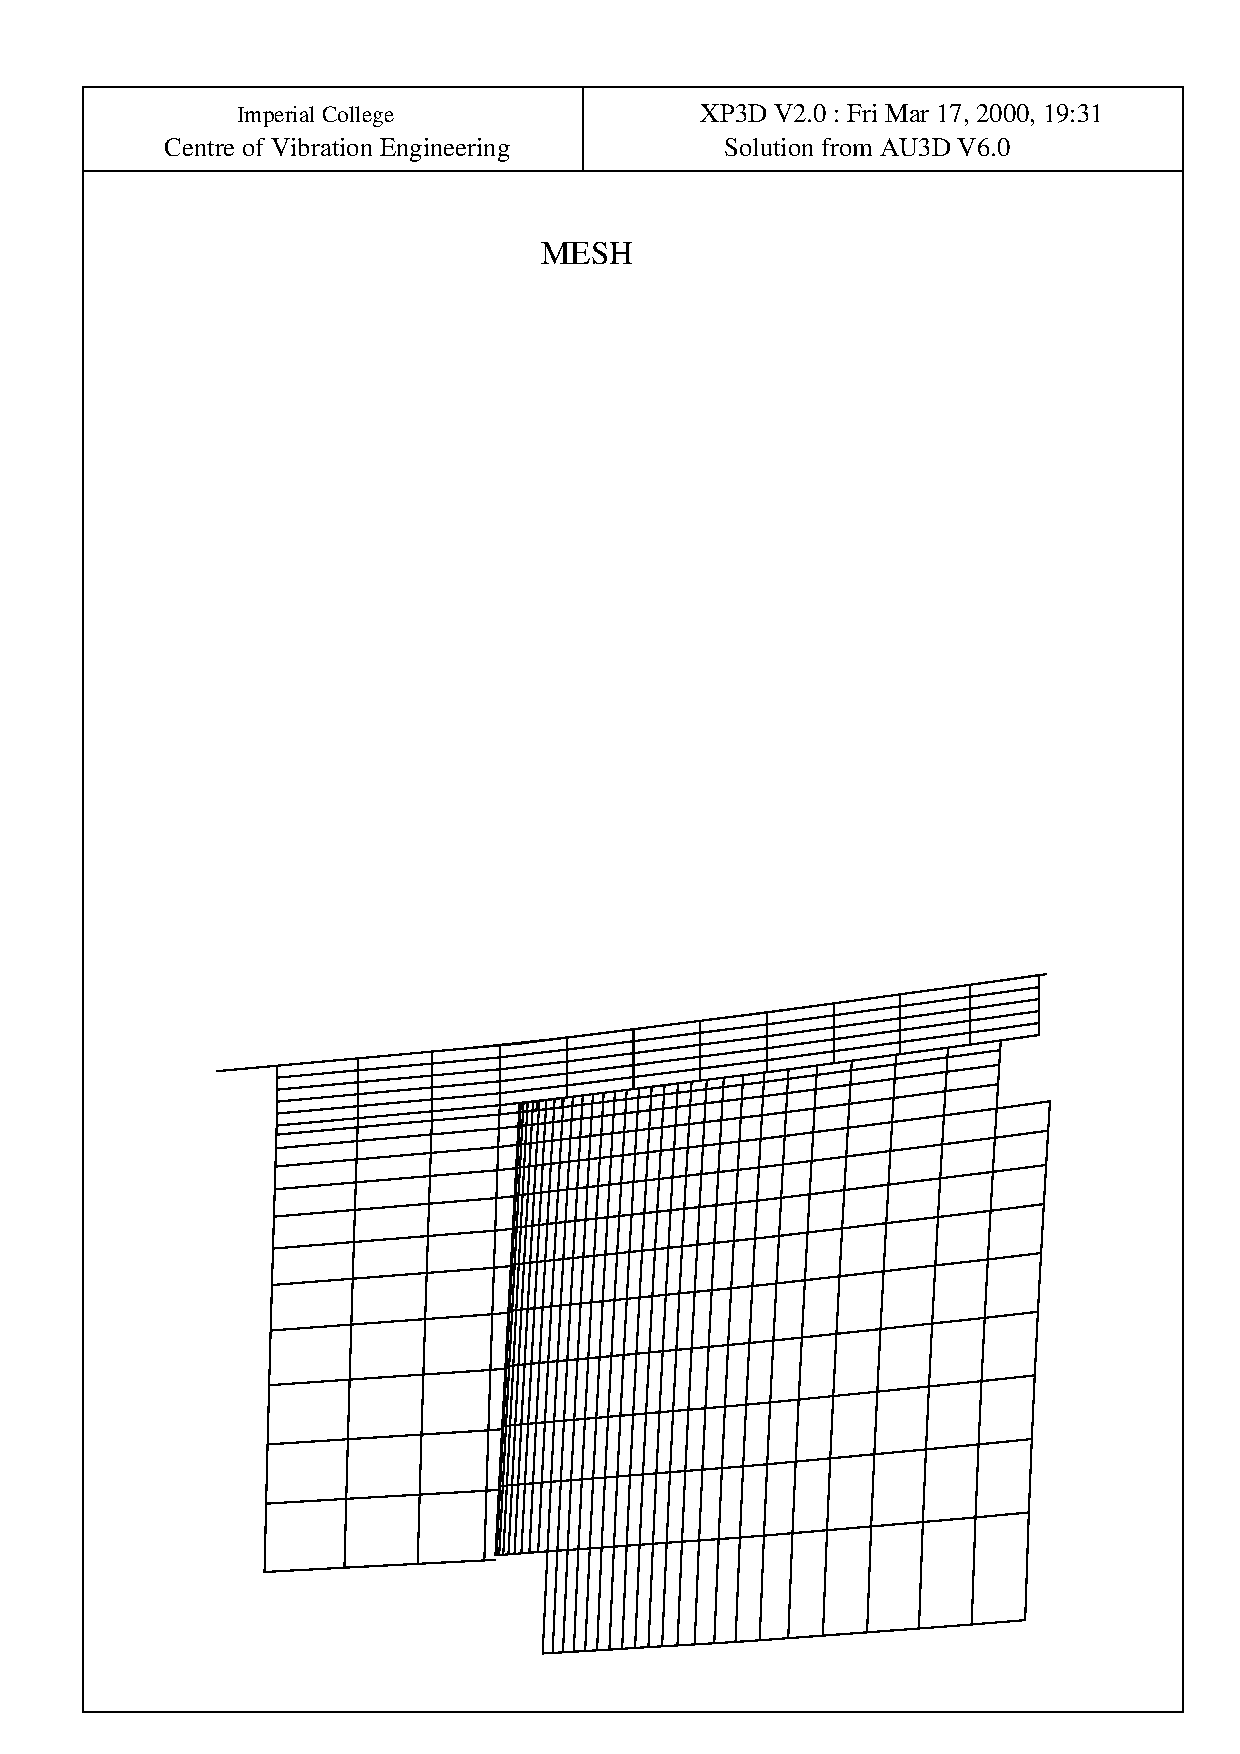
\includegraphics[width=70mm,clip=t]{CHAP_RT27/FIGURE/mesh3d_4.pdf}}
        &
    \subfigure[Tip-section]
       {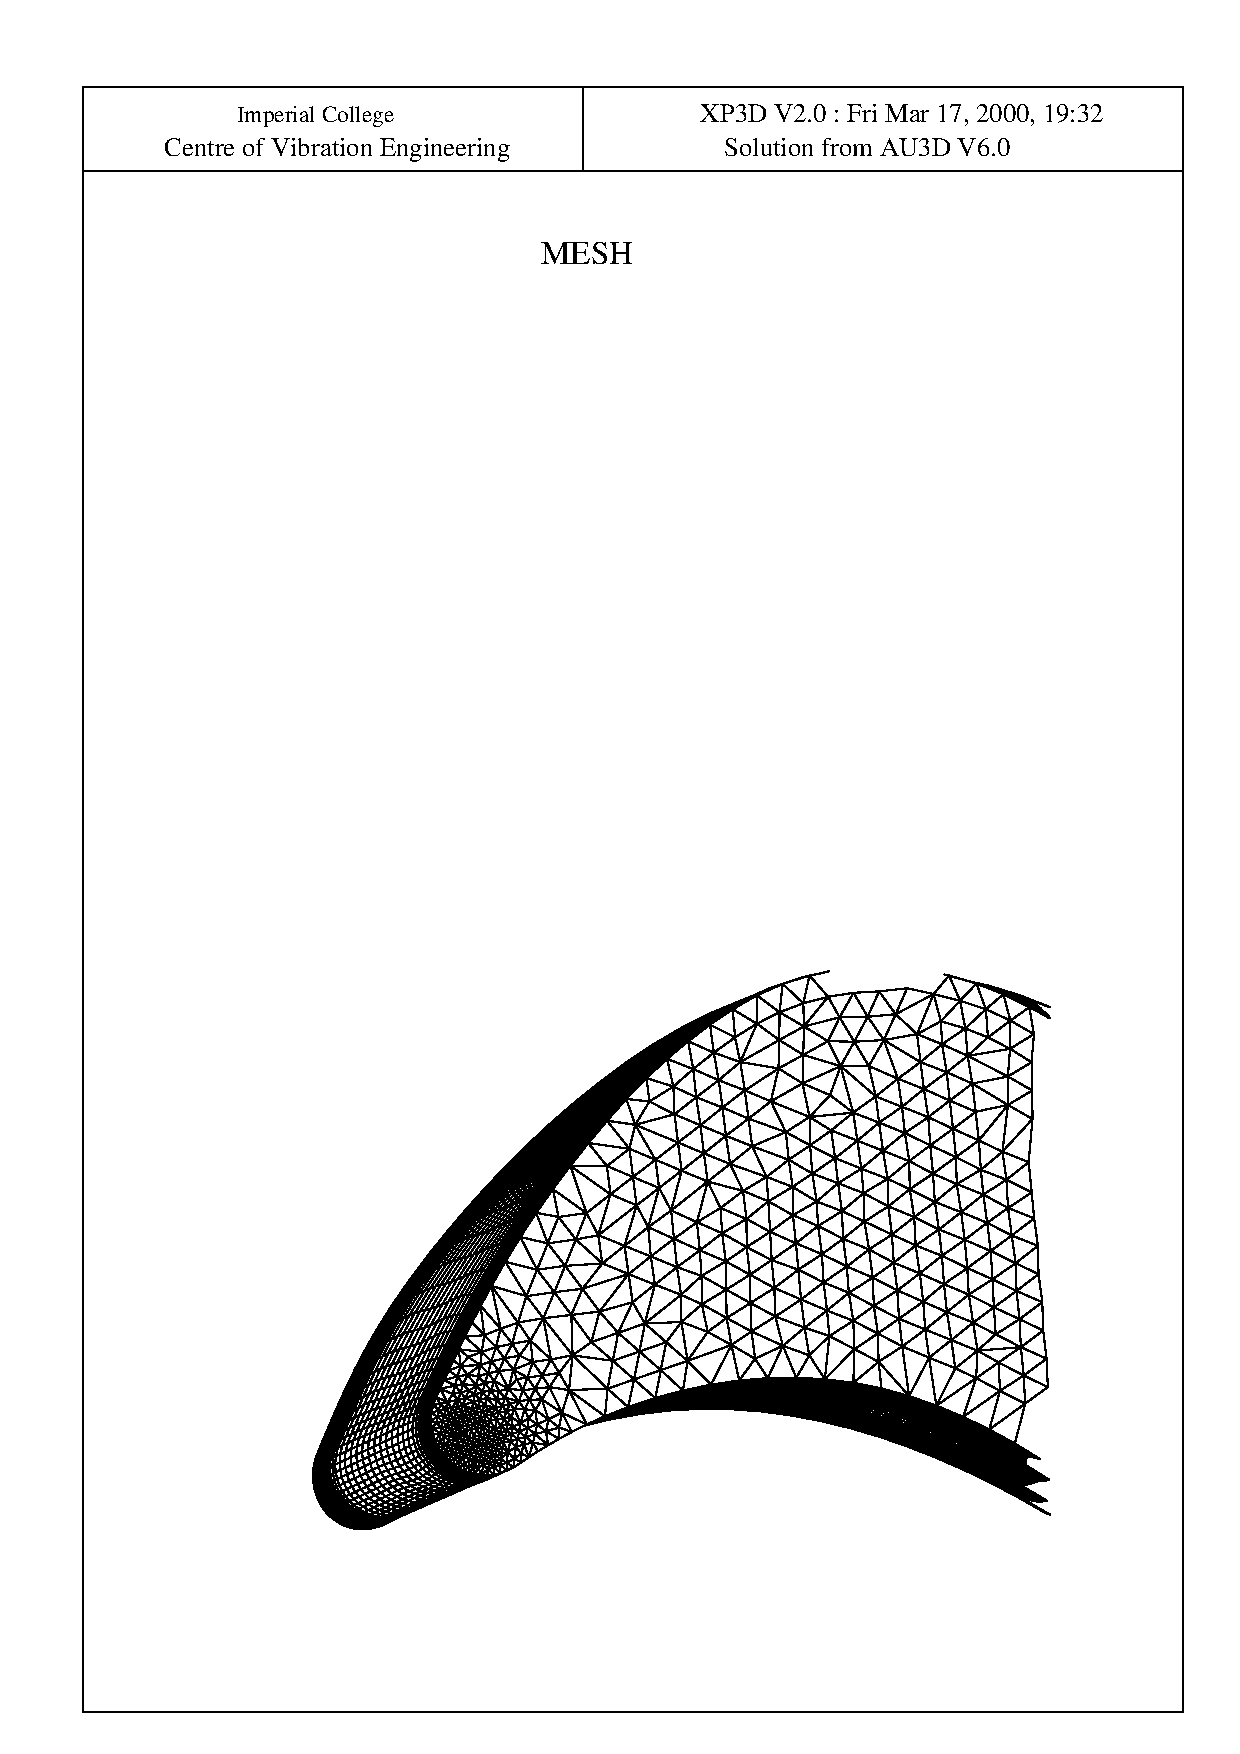
\includegraphics[width=70mm,clip=t]{CHAP_RT27/FIGURE/mesh3d_5.pdf}}
  \end{tabular}
 \end{center}
 \vspace{-8mm}
 \caption{Computational mesh at tip end wall of RT27a rotor blade}
 \label{rt27_mesh2.fig}
\end{figure}
%
 Both grids have 48 points in the radial direction, the
 locations at the NGV-outlet and rotor-inlet being identical
 (Fig. \ref{rt27_mesh1.fig}b).
 As shown in Fig. \ref{rt27_mesh2.fig}a, 42 of the radial grid levels,
 define the rotor geometry while the remaining six are positioned
 in the tip-gap region.
 Fig. \ref{rt27_mesh2.fig}b shows the triangulation of the
 rotor tip section.

 Both the NGV and the rotor boundary layer regions are discretised by
 a twelve-layer of O-type mesh formed by hexahedra elements.
 Such a resolution is sufficient for a viscous computation
 which uses the law of the wall to evaluate the wall shear stresses.

 Fig. \ref{rt27_mesh3.fig} shows the mid-height radial section
 of the computational mesh.
 The NGV grid contains 4,717 points per radial level which yields a total
 of 226,416 points.
 The inclusion of the NGV passage in the steady-state computation
 is mainly justified by the need of (i) predicting a correct steady-state
 inlet conditions for the rotor passage and (ii) the evaluation of the
 spatial non-uniformities at the NGV-outlet.
 For these reason the NGV-grid is refined in the trailing-edge
 and outflow regions.
%
\begin{figure}[ht]
 \centerline{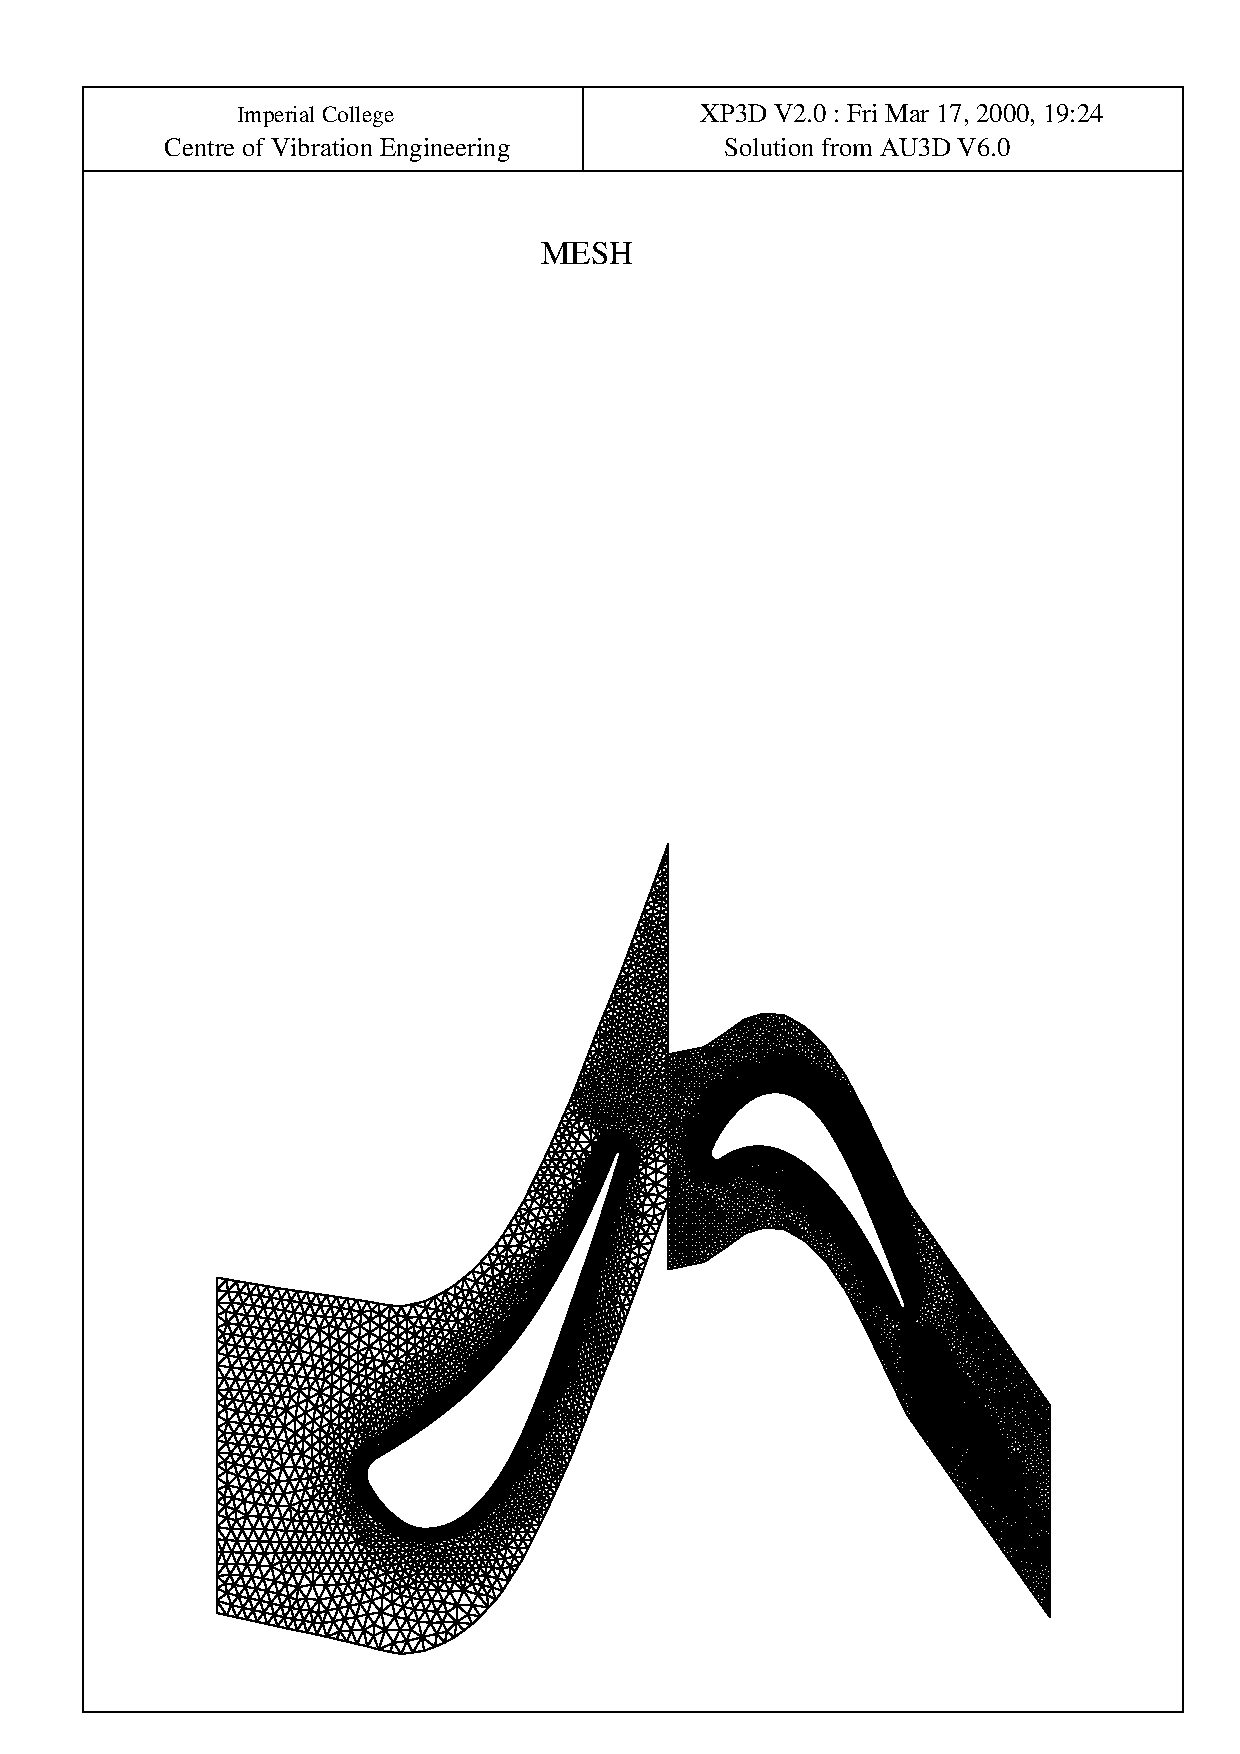
\includegraphics[width=140mm,clip=t]{CHAP_RT27/FIGURE/mesh3d_2.pdf}}
 \caption{Computational mesh at mid-height section of RT27a turbine stage}
 \label{rt27_mesh3.fig}
\end{figure}
%
 The rotor grid contains 338,244 points distributed in the following way:
 each one of the six radial section in the tip-clearance region
 contains 7,850 points while each one of the remaining 42 sections
 contains 6,932 points. The number of points positioned in the
 rotor tip section of Fig. \ref{rt27_mesh2.fig}b is 918.
%
\begin{table}
\vspace{5mm}
\begin{center}
\begin{tabular}{|l|l|}\hline\hline
 Periodic boundary (axial direction) & 126\\ \hline
 Inflow boundary (tangential direction)& 41\\ \hline
 Outflow boundary (tangential direction)& 43\\ \hline
 Blade suction side (axial direction)& 110\\ \hline
 Blade pressure side (axial direction)& 108\\ \hline
\hline
\end{tabular}
\end{center}
\caption{Number of point on domain boundaries of RT27a rotor blade}
\label{rotor_mesh.tab}
\end{table}
%
 Table \ref{rotor_mesh.tab} lists the number of points in each boundary
 of a rotor radial section.

 The tip clearance grid is relatively coarse since the main interest
 is not to predict accurately the structure of the tip-leakage flow,
 but only to take into account its main effect on the
 hub-to-tip pressure distribution.
 Since the main parameters which can affect the pressure distribution
 towards the tip are the size of the clearance and the
 pressure jump across the blade,
 the tip-grid of Fig. \ref{rt27_mesh2.fig}
 is considered to be sufficient for the purposes of the current analysis.
%
%
%
\subsection{Boundary conditions and computational details}
\label{rt27_boundary.subsec}
%
 The boundary conditions, together with the rotor rotational speed,
 specify at which point in the turbine stage characteristic the calculation
 is performed. The nominal design condition has been chosen for
 this numerical analysis. The rotor rotational speed is the one
 reported in table \ref{rt27.tab}. The NGV inlet conditions are the
 following: constant stagnation
 pressure ($p\sm{01}$ in table \ref{rt27.tab}), constant
 stagnation temperature ($T\sm{01}$ in table \ref{rt27.tab}),
 flow direction without tangential component ($\alpha\sm{x\theta} = 0$) and
 flow angle in the $x-r$ plane reported in Fig. \ref{bcond.fig}a.
 The final boundary condition is applied at the rotor outlet where
 the static pressure distribution of Fig \ref{bcond.fig}b is specified.
 A sequence of three agglomerated grid levels were generated for both the
 NGV and the rotor domains so that a 4-grid W-cycle algorithm was used
 for the steady state computations.
 Starting from free-stream conditions the computation took around 300
 multigrid cycles to converge. The calculation was
 performed on a 500 MHz DEC Alpha machine where the 300 multigrid cycles
 were completed in about 8 hours.
 The average $y+$, which indicates the the resolution of the viscous body fitted
 O-grid, was of around 150 while the maximum was $\approx 500$.
 Both these values are within the logaritmic part of the turbulent
 boundary layer thus justifying the grid-resolution in this region.
%
\begin{figure}[ht]
 \begin{center}
  \begin{tabular}{cc}
    \hspace{-10mm}
    \subfigure[NGV inlet flow angle in the $x-r$ plane]
       {\includegraphics[height=60mm,clip=t]{CHAP_RT27/FIGURE/alphaxr.pdf}}
        &
    \subfigure[Rotor outlet static pressure]
       {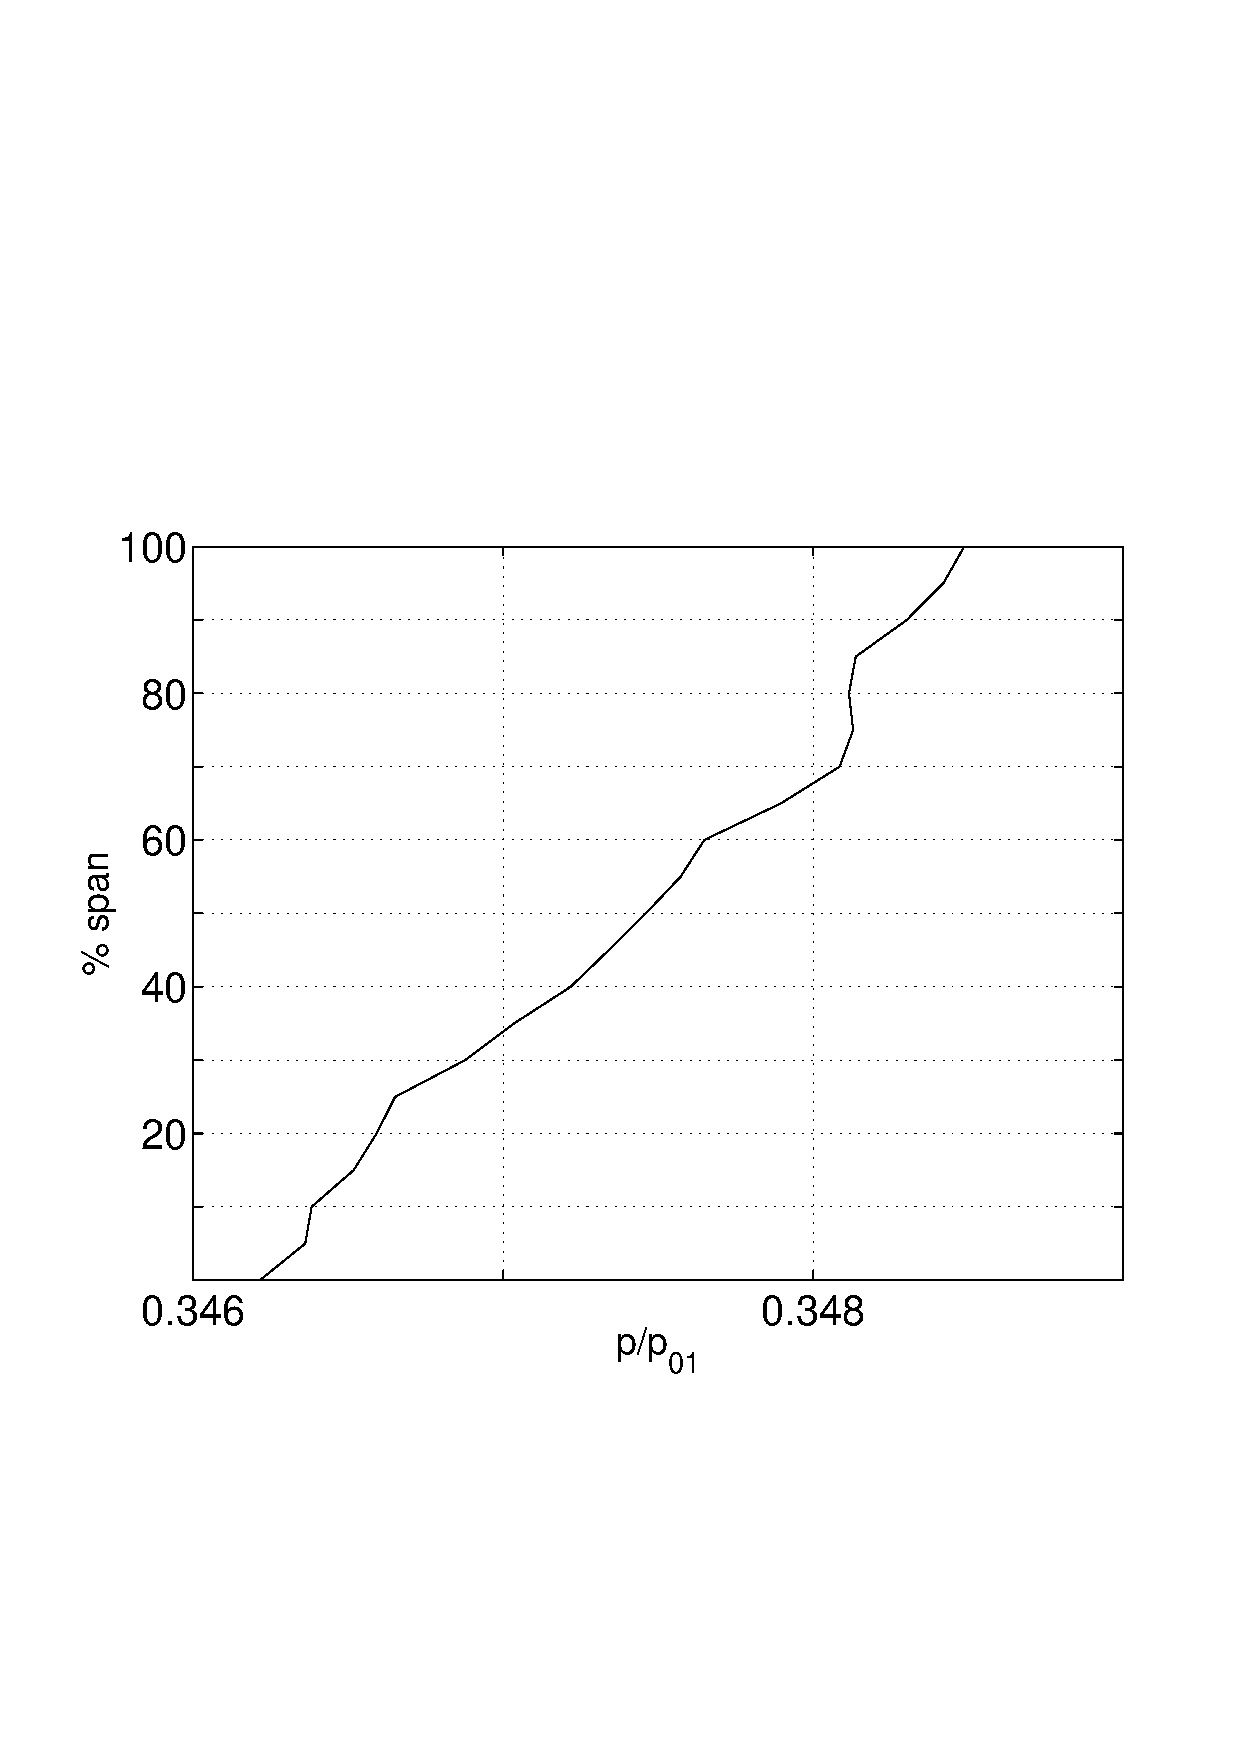
\includegraphics[height=60mm,clip=t]{CHAP_RT27/FIGURE/outpres.pdf}}
  \end{tabular}
 \end{center}
 \vspace{-6mm}
 \caption{Boundary conditions of RT27a turbine stage}
 \label{bcond.fig}
\end{figure}
%
%
%
\subsection{Results of steady-state flow calculation}
\label{rt27_steady.subsec}
%
\begin{figure}[ht]
 \begin{center}
  \begin{tabular}{cc}
    \subfigure[Pressure side]
       {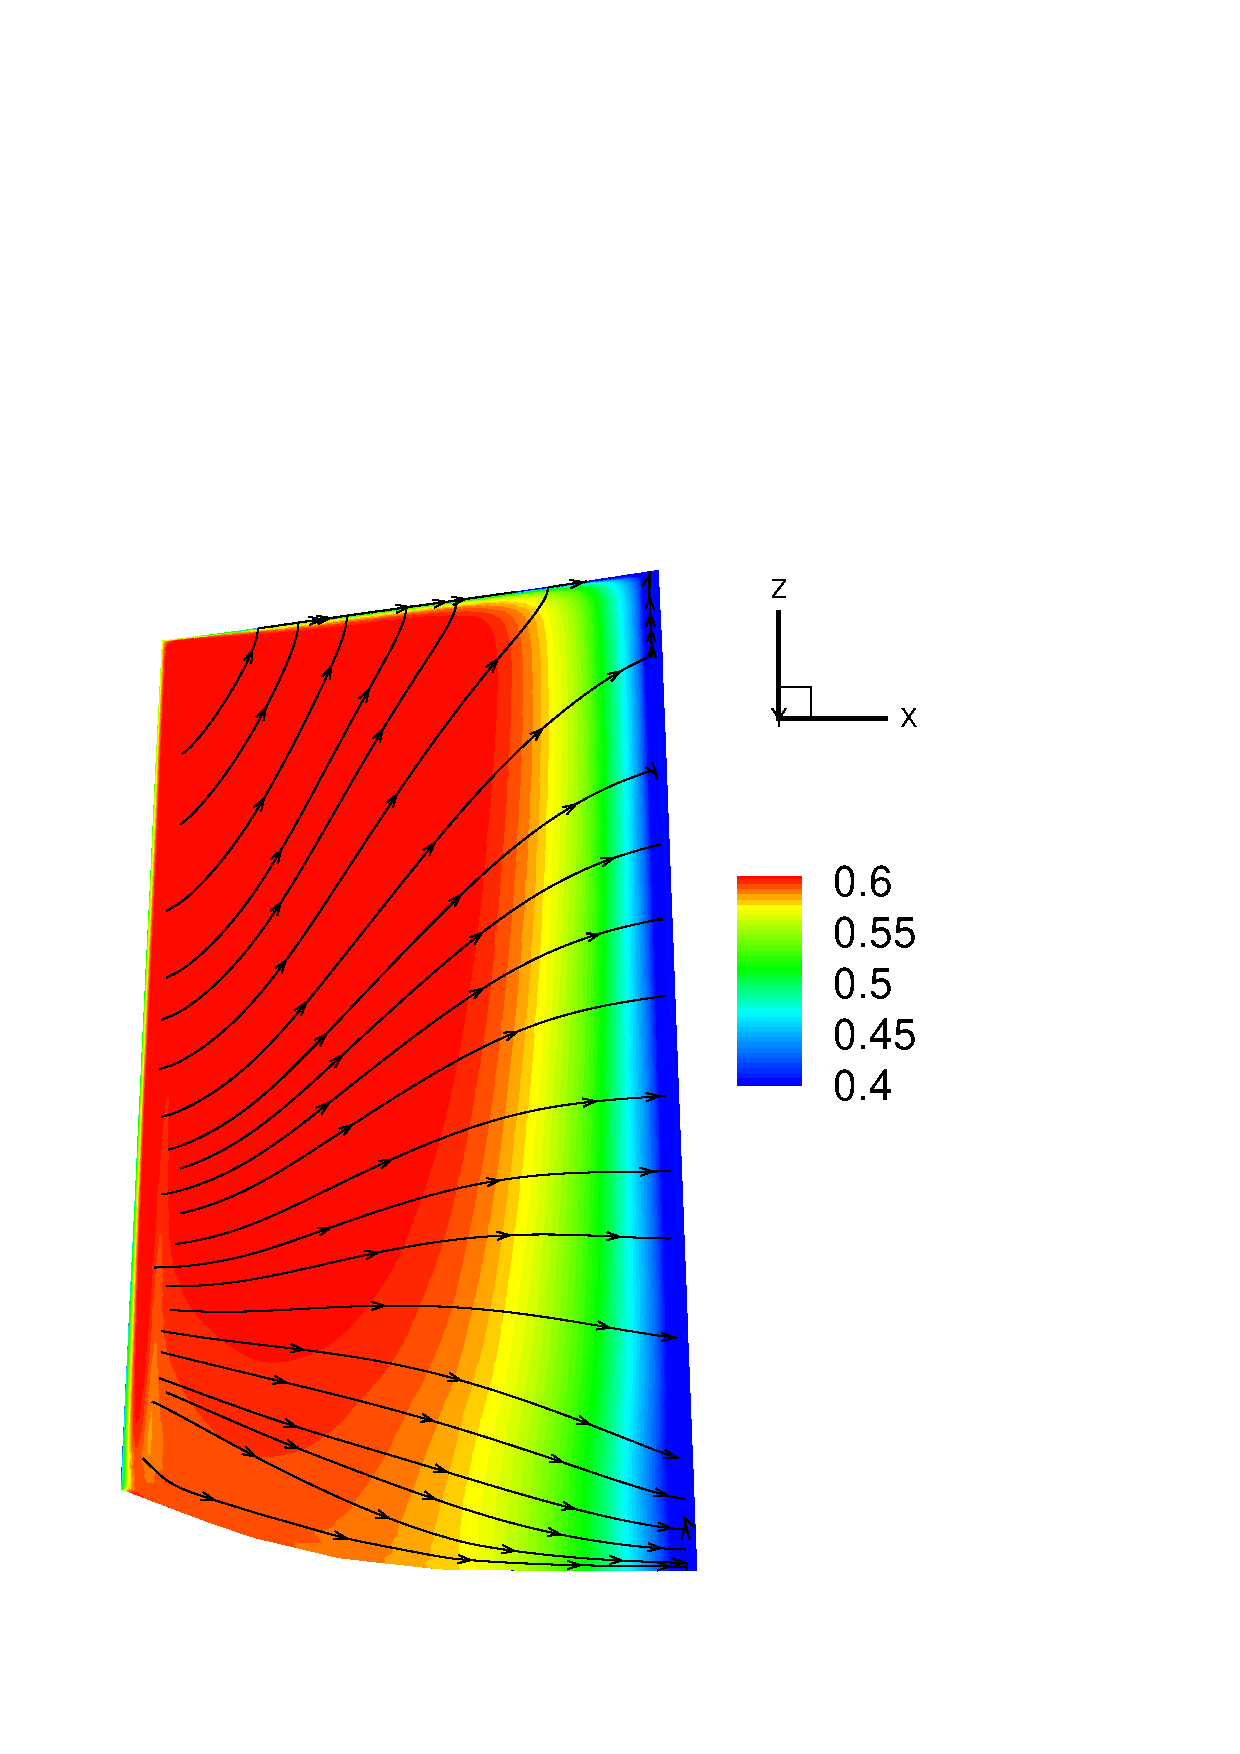
\includegraphics[width=75mm,clip=t]{CHAP_RT27/FIGURE/rotor_traces_pres.pdf}}
        &
    \subfigure[Suction side]
       {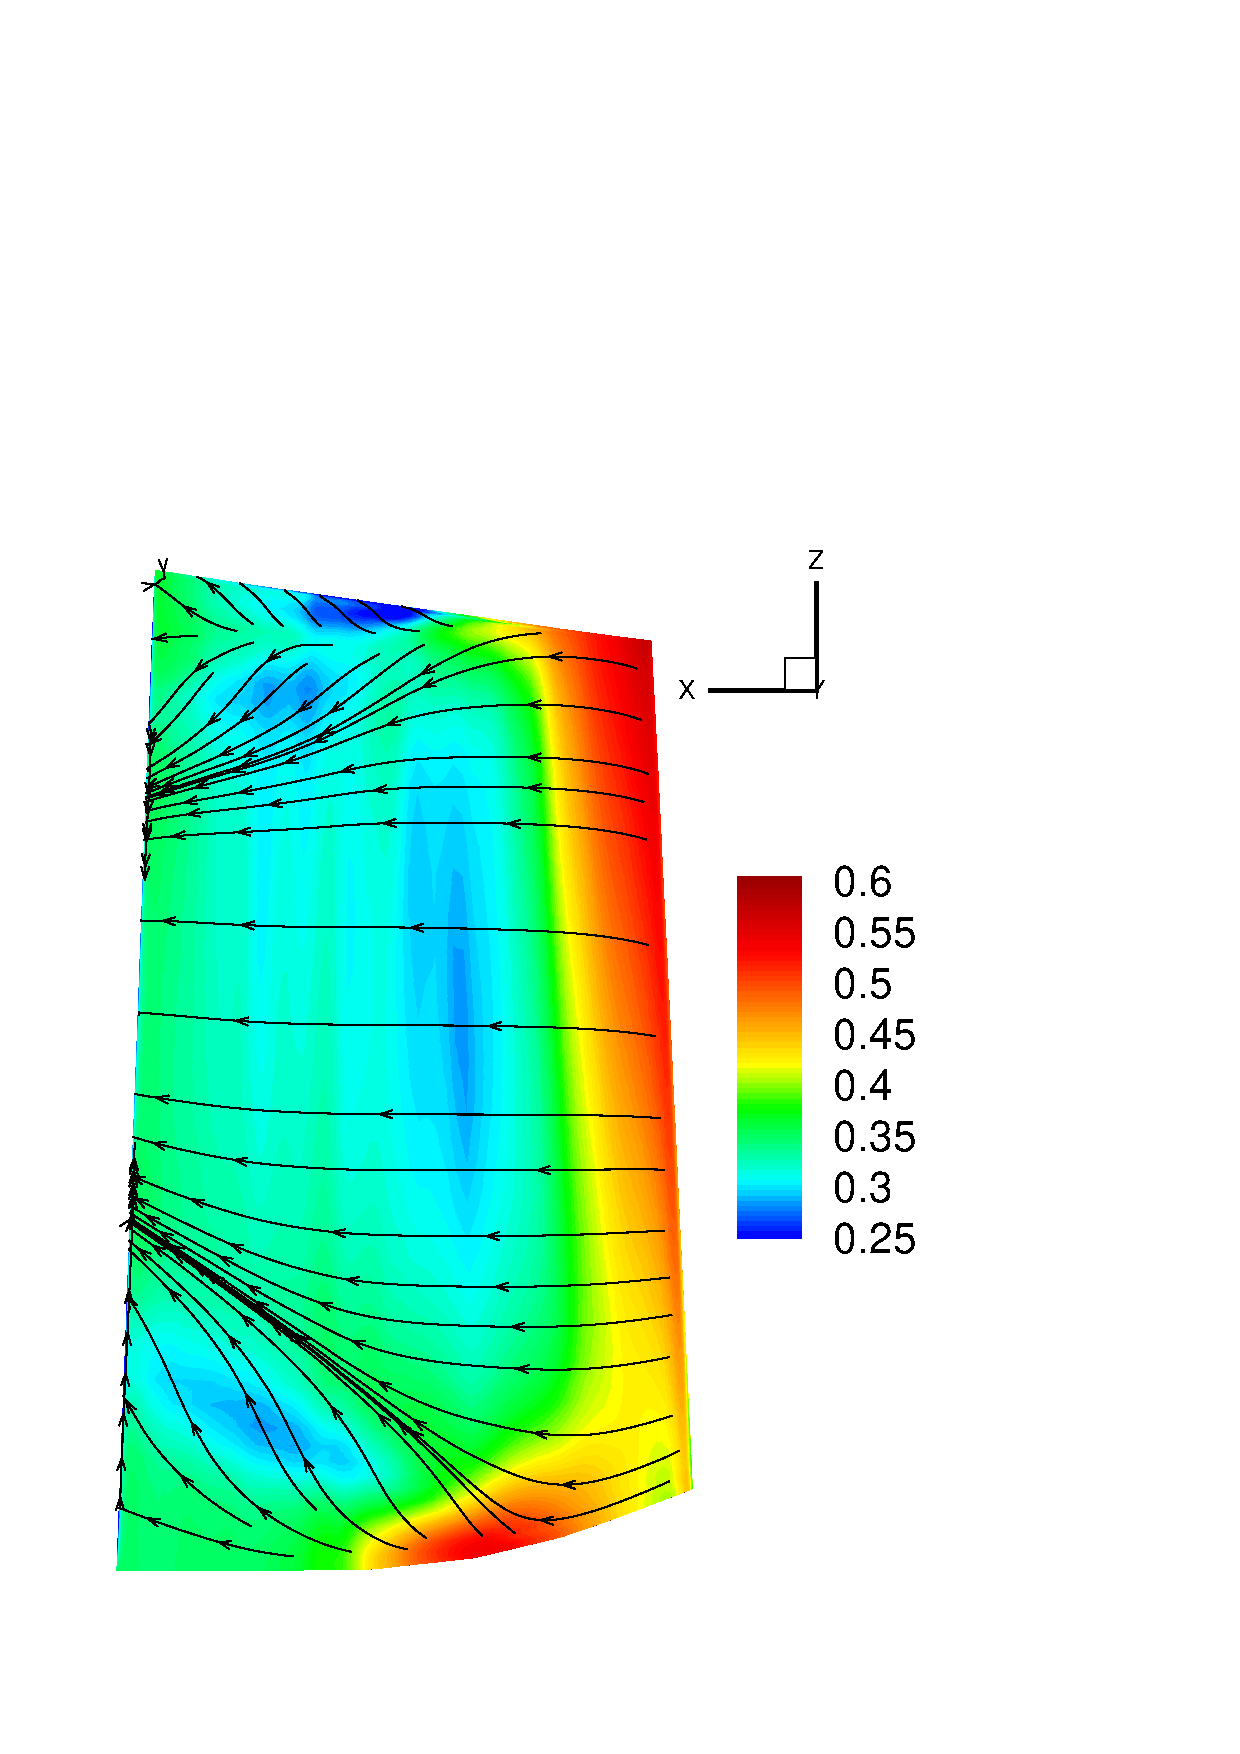
\includegraphics[width=75mm,clip=t]{CHAP_RT27/FIGURE/rotor_traces_suct.pdf}}
  \end{tabular}
 \end{center}
 \vspace{-6mm}
 \caption{Steady state pressure contours $\frac{p}{p\sm{01}}$
          and particle traces on the RT27a rotor surface}
 \label{rotor_blade_traces.fig}
\end{figure}
%
 Fig. \ref{rotor_blade_traces.fig} shows the computed steady state static
 pressure on the rotor blade surface together with particle traces.
 The pressure distribution on the pressure surface is, in the main,
 2D even though the particle traces
 show a significant radial component, especially towards the tip region
 where the tip-clearance pressure jump tends to drive the flow from the pressure
 side towards the suction side of the blade.
 The 3D effects are much more evident from the suction
 surface (Fig. \ref{rotor_blade_traces.fig}b). The flow behaves in a
 2D way only in the middle section, while
 secondary flow effects are very much evident towards both end walls.
 In particular, the separation line caused by the suction side
 leg of the horseshoe vortex is clearly visible at the hub end wall.
 The migration of the separation line
 towards mid-section is caused by the rotation of the passage vortex.
 Such a separation line is also present at the tip end wall but
 the flow pattern is more complicated.
 This is caused by the interaction of the passage and tip-leakage
 vortices which result in counter-rotating flow structures.
 Section \ref{rt27_secondaryflow.subsec} will present a more detailed
 discussion of these secondary flow effects.

 Fig. \ref{rotor_blade_machis1.fig} shows a comparison of predicted and measured
 isentropic Mach number blade distributions at mid-height section.
%
\begin{figure}
  \centerline{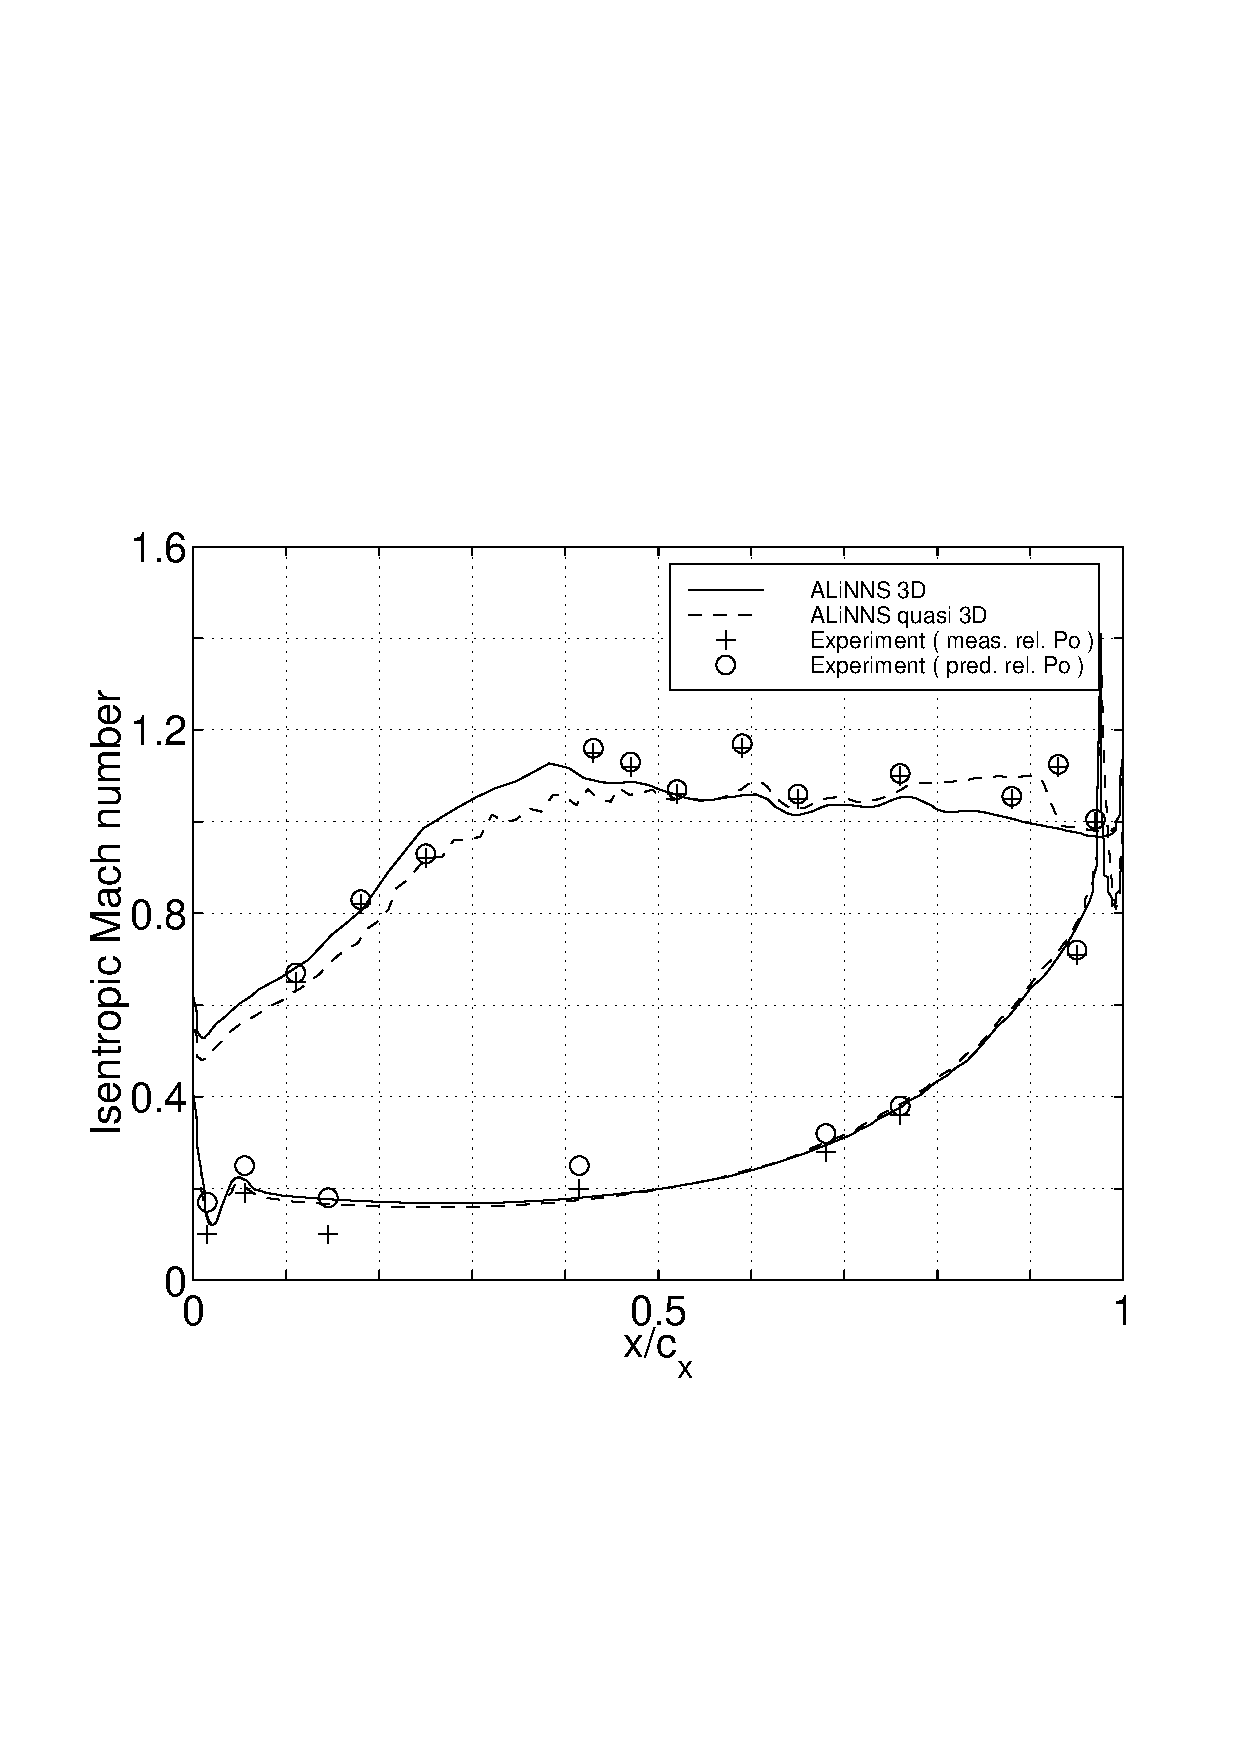
\includegraphics[width=100mm,clip=t]{CHAP_RT27/FIGURE/mid.pdf}}
  \caption{Isentropic steady-state Mach number distribution at
           mid-height section of RT27a rotor blade}
  \label{rotor_blade_machis1.fig}
\end{figure}
%
 The two experimental Mach number distributions are calculated from
 the time-mean unsteady static pressures but using two different values of
 the rotor-relative total pressures at the leading-edge: the experimental
 and the computed values.
 The discrepancy between the two measured curves can be considered to
 be an indicator of the experimental sensitivity to the rotor relative inlet
 total pressure.
 Fig. \ref{rotor_le.fig} shows the comparison between the measured and computed
 leading-edge pressure values along the radial direction.
 In addition to the distribution obtained from the 3D
 steady-state computation,
 Fig. \ref{rotor_blade_machis1.fig} reports the result of a quasi-3D
 calculation performed at mid-height section.
 The true 3D result agrees, with the measurements,
 better in the forward part
 of the blade suction surface while it overestimates the
 exit pressure.
%
\begin{figure}
  \centerline{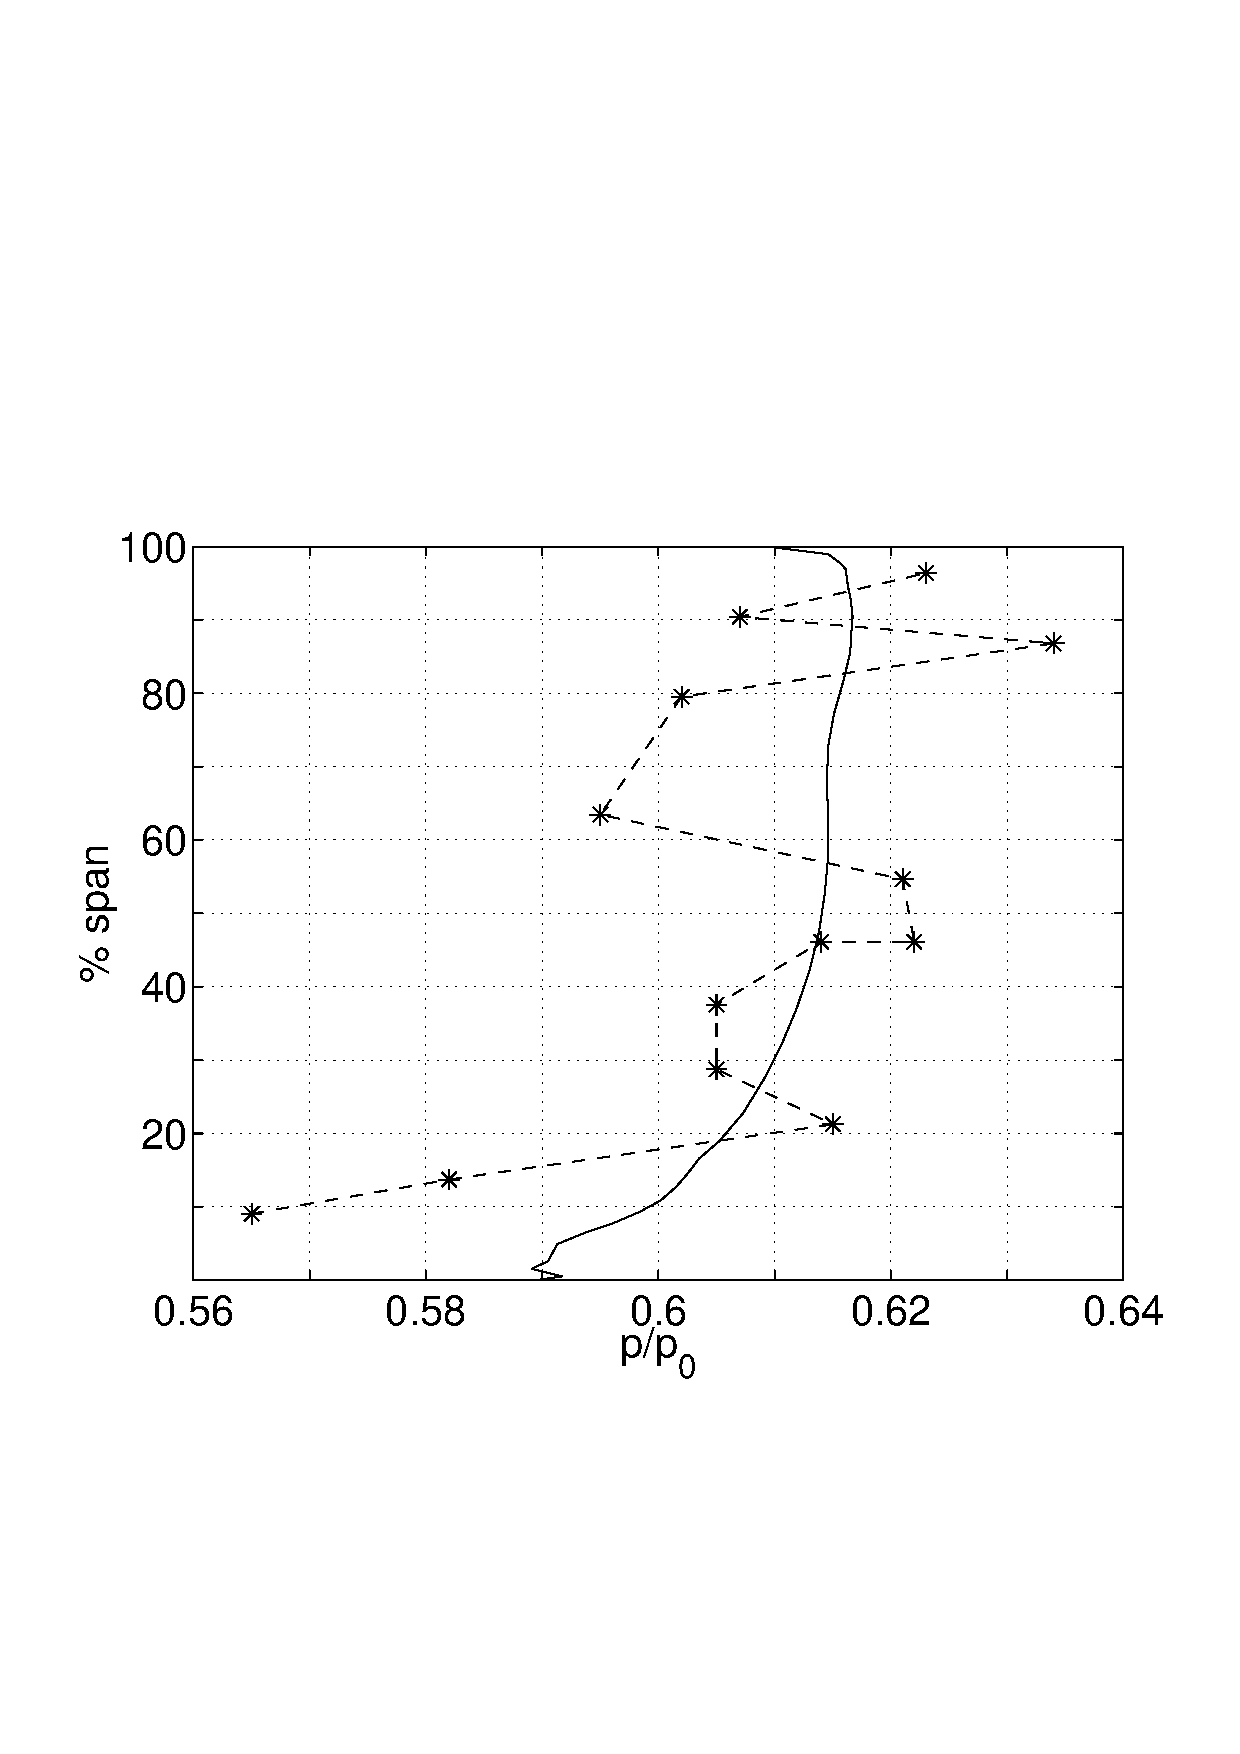
\includegraphics[width=100mm,clip=t]{CHAP_RT27/FIGURE/rot_le.pdf}}
  \caption{RT27a rotor leading-edge pressure levels. (*) Leading-edge kulite
           measured data, (-) computed}
  \label{rotor_le.fig}
\end{figure}
%
 Fig. \ref{rotor_blade_machis2.fig} shows a comparison of the predicted
 isentropic Mach number blade distributions at 5, 10, 90 and 95\%
 spans with the time-averaged measured data.
 The overall agreement is reasonably good although some discrepancies
 are worth mentioning.
 As for the mid-height blade distribution of Fig. \ref{rotor_blade_machis1.fig},
 the computed results in the trailing-edge region of the suction surface
 underestimate the measured isentropic Mach number.
 The reasons for such discrepancies are not entirely clear. However, it should
 be noted that experimental data represent averaged unsteady flow which,
 under certain circumstances may be different from the true steady flow.
 This is probably the case of regions where shock waves are present, i.e.
 towards the trailing-edge region of the suction surface.
%
%
\begin{figure}[ht]
 \begin{center}
  \begin{tabular}{cc}
    \subfigure[Root section]
       {\hspace{-10mm}\includegraphics[width=75mm,clip=t]{CHAP_RT27/FIGURE/hub.pdf}}
        &
    \subfigure[Mid-root section]
       {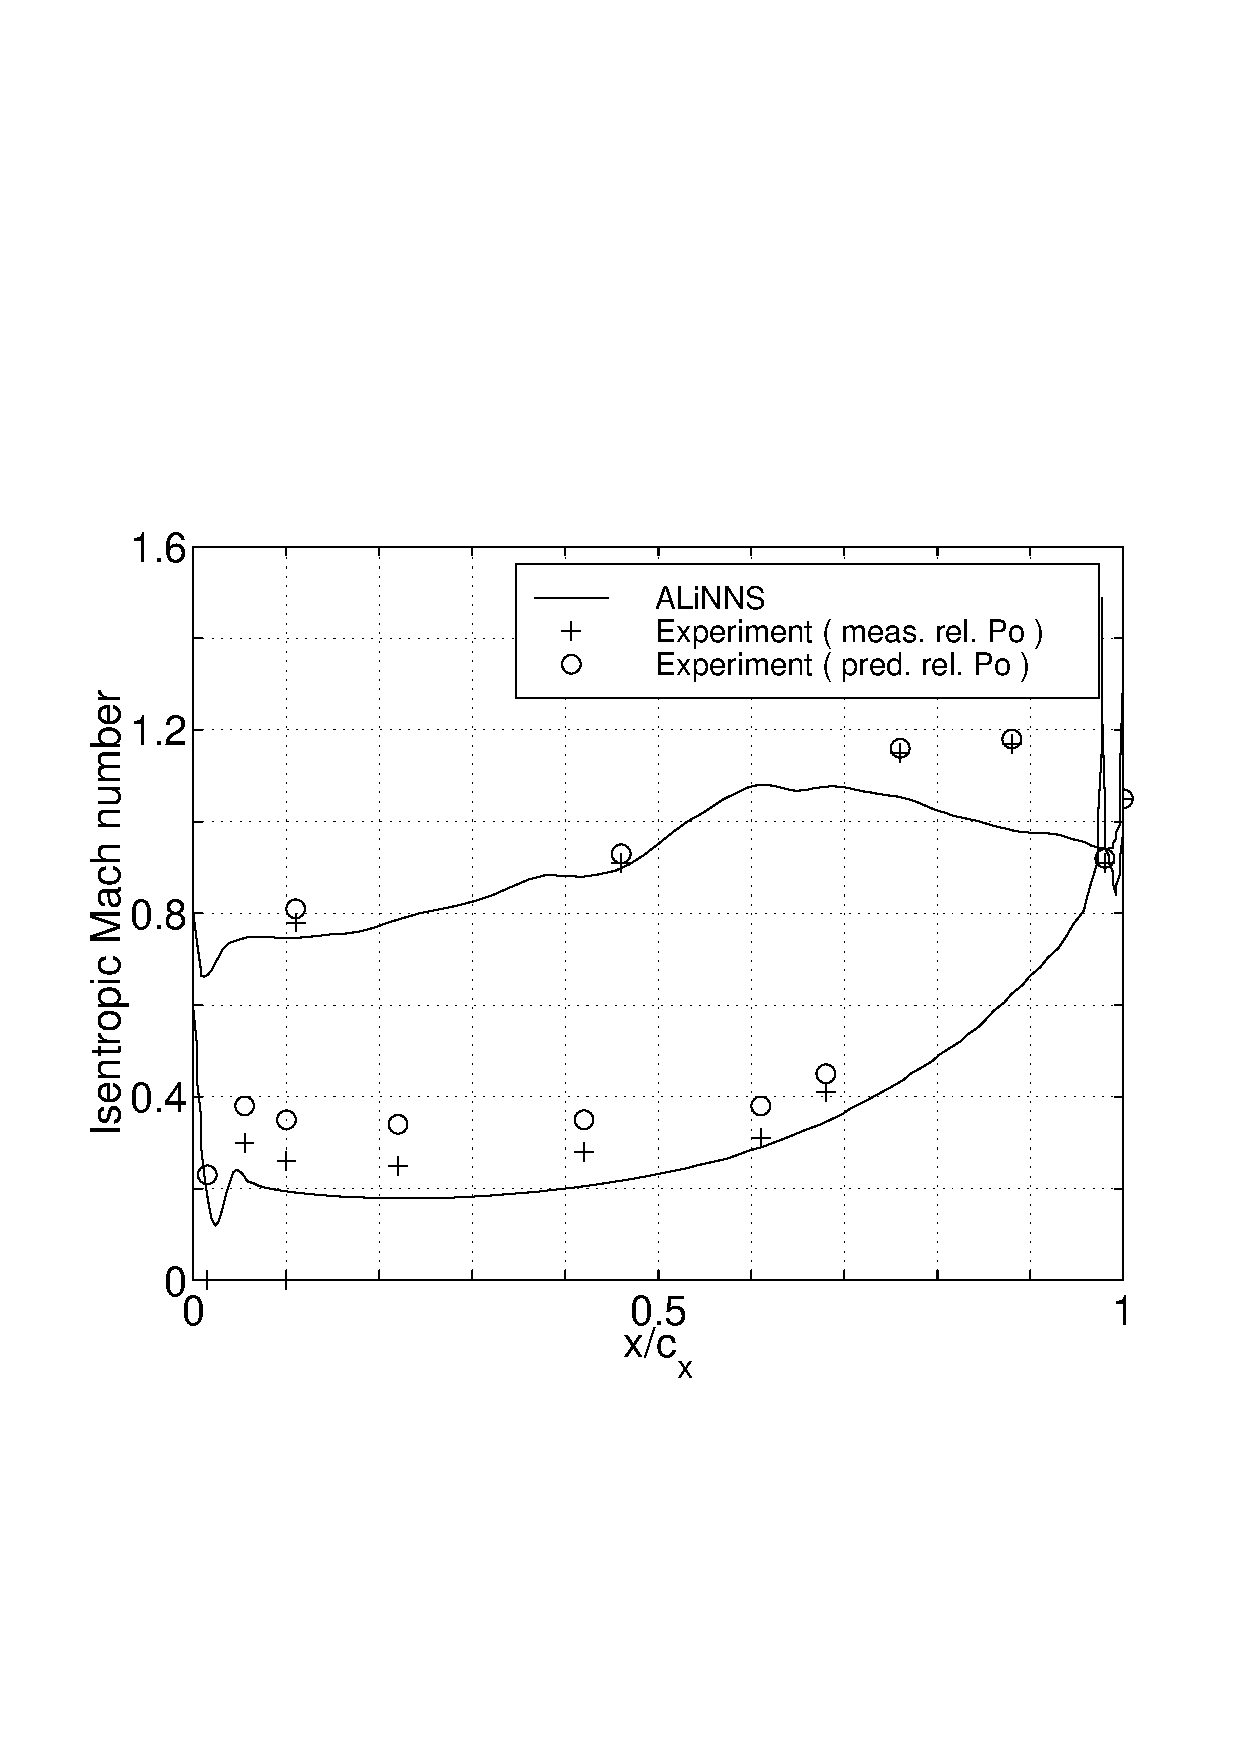
\includegraphics[width=75mm,clip=t]{CHAP_RT27/FIGURE/midhub.pdf}}
       \vspace{-4mm}\\
    \subfigure[Mid-tip section]
       {\hspace{-10mm}\includegraphics[width=75mm,clip=t]{CHAP_RT27/FIGURE/midtip.pdf}}
        &
    \subfigure[Tip section]
       {\includegraphics[width=75mm,clip=t]{CHAP_RT27/FIGURE/tip.pdf}}
  \end{tabular}
 \end{center}
 \vspace{-8mm}
 \caption{RT27a rotor blade: isentropic steady-state Mach number distribution
          at different span-wise positions}
 \label{rotor_blade_machis2.fig}
\end{figure}
%

 One feature that is common to Figs. \ref{rotor_blade_machis1.fig}
 and \ref{rotor_blade_machis2.fig} is that the pressure-side isentropic
 Mach number distribution is almost the same for all span-wise
 positions, a feature that is also evident from Fig. \ref{rotor_blade_traces.fig}a.
 The suction-side results show considerable deviations from the base 2D flow
 due to secondary and tip-leakage flows effects.
 Fig. \ref{rotor_blade_machis2.fig}a shows that forward position of
 the suction side is unloaded relative to midspan values.
 At mid-root, the unloading in the forward position is less pronounced
 and the results are closer to the midspan values.
 This trend of a increasing load on the forward position continues all the way
 to the tip.
%
%
%
%
%
\subsection{Secondary and tip-clearance flow}
\label{rt27_secondaryflow.subsec}
%
 Three main vortices were identified in the rotor blade passage:
 the {\em horseshoe} vortex, the {\em passage} vortex and the
 {\em tip-leakage} vortex.
 The formation of first two vortices is connected to the presence
 of velocity gradients near the end wall boundary layers while
 the tip-leakage vortex is caused by the fast moving flow in the gap region.

 The horseshoe vortex has two legs, namely the suction and pressure side legs.
 This vortex is formed around the leading-edge of the blade at the end wall
 regions, in the same way as around any blunt body with its axis
 perpendicular to the wall. The high energy fluid, at the edge
 of the end wall boundary layer, flows away from the leading-edge
 stagnation point, not only around the blade, but also downwards because of
 the lower energy of the fluid below.
 When this high energy fluid reaches the end wall, it flows upstream forming
 a saddle point where the upstream flow separates form the surface.
 Fig. \ref{rotor_hub_traces.fig} shows the static pressure contours as well
 as the particle traces at $1\%$ span. The two separation lines
 caused by the pressure and the suction leg of the horseshoe vortex can
 be seen clearly.
 The suction side leg remains close to the blade and then, as indicated in
 Fig. \ref{rotor_blade_traces.fig}, travels up the suction surface,
 while the pressure side leg crosses the blade passage to the suction
 side of the other blade.
%
\begin{figure}
 \centerline{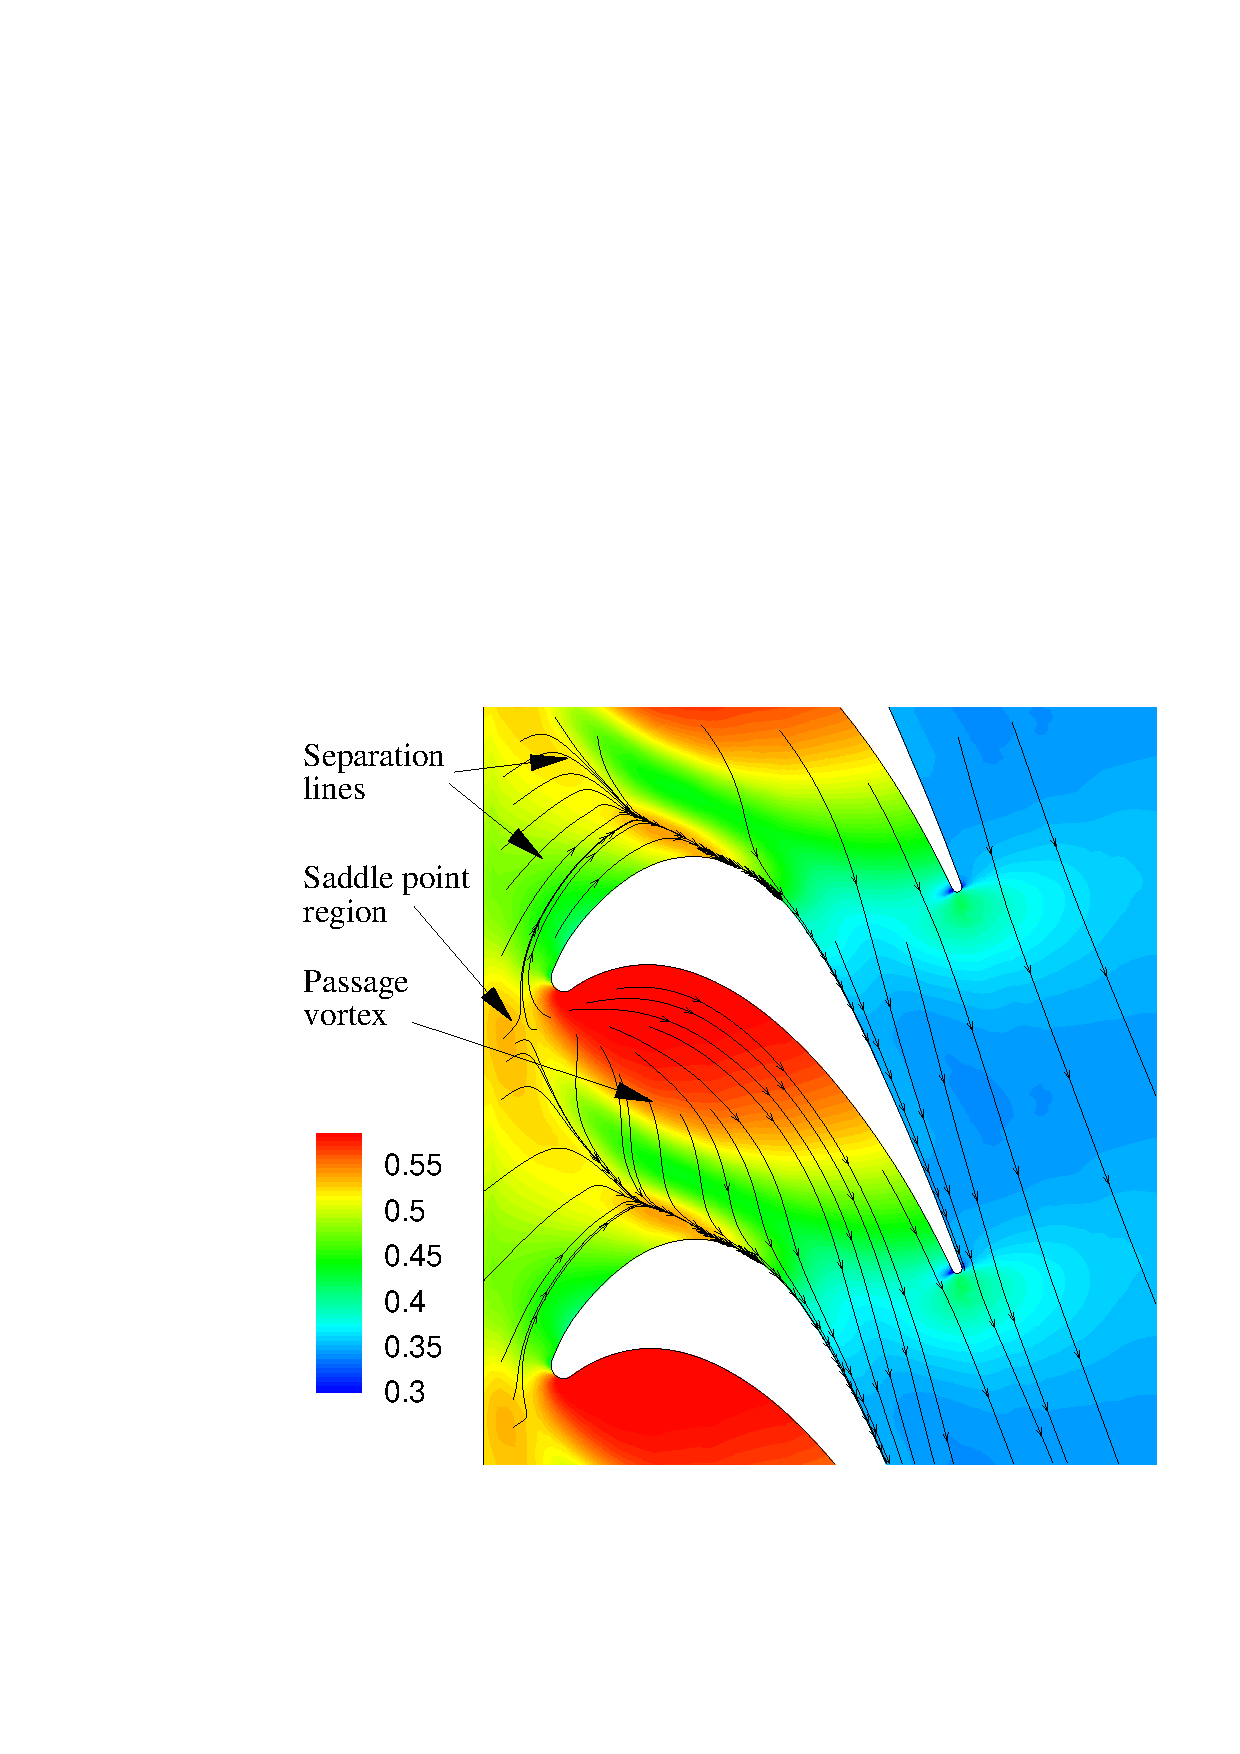
\includegraphics[width=100mm]{CHAP_RT27/FIGURE/rotor_hub_traces.pdf}}
 \caption{Steady state pressure contours $\frac{p}{p\sm{01}}$
          and particle traces at $1\%$ span of RT27a rotor blade}
 \label{rotor_hub_traces.fig}
\end{figure}
%
 The detail is very complex, but the same main features were noted
 by other researchers (Sieverding \citeyearNP{Sieverding:1},
 Gregory-Smith \citeyearNP{Gregory:1}).

 The passage vortex is associated with the turning
 of the vorticity vector, and its main effect occurs in the middle of
 the passage. Its rotation is in the same sense as the pressure side leg
 of the horseshoe vortex and the two evolve and merge together.
 Fig. \ref{rotor_passage_traces.fig} shows the particle traces at two
 consecutive axial planes. At an axial plane $15\%$ chord downstream
 of the leading-edge, a recirculating flow pattern,
 formed by the passage vortex and pressure side leg of the
 horseshoe vortex, is centered in the middle of the passage.
 Within the blade passage the vortex is convected by its own flow field
 from the pressure surface towards the suction surface as indicated
 in Fig. \ref{rotor_passage_traces.fig}b.
%
%
%
\begin{figure}[ht]
 \begin{center}
  \begin{tabular}{lll}
    \hspace{-10mm}
    \subfigure[$15\%$ axial chord]
       {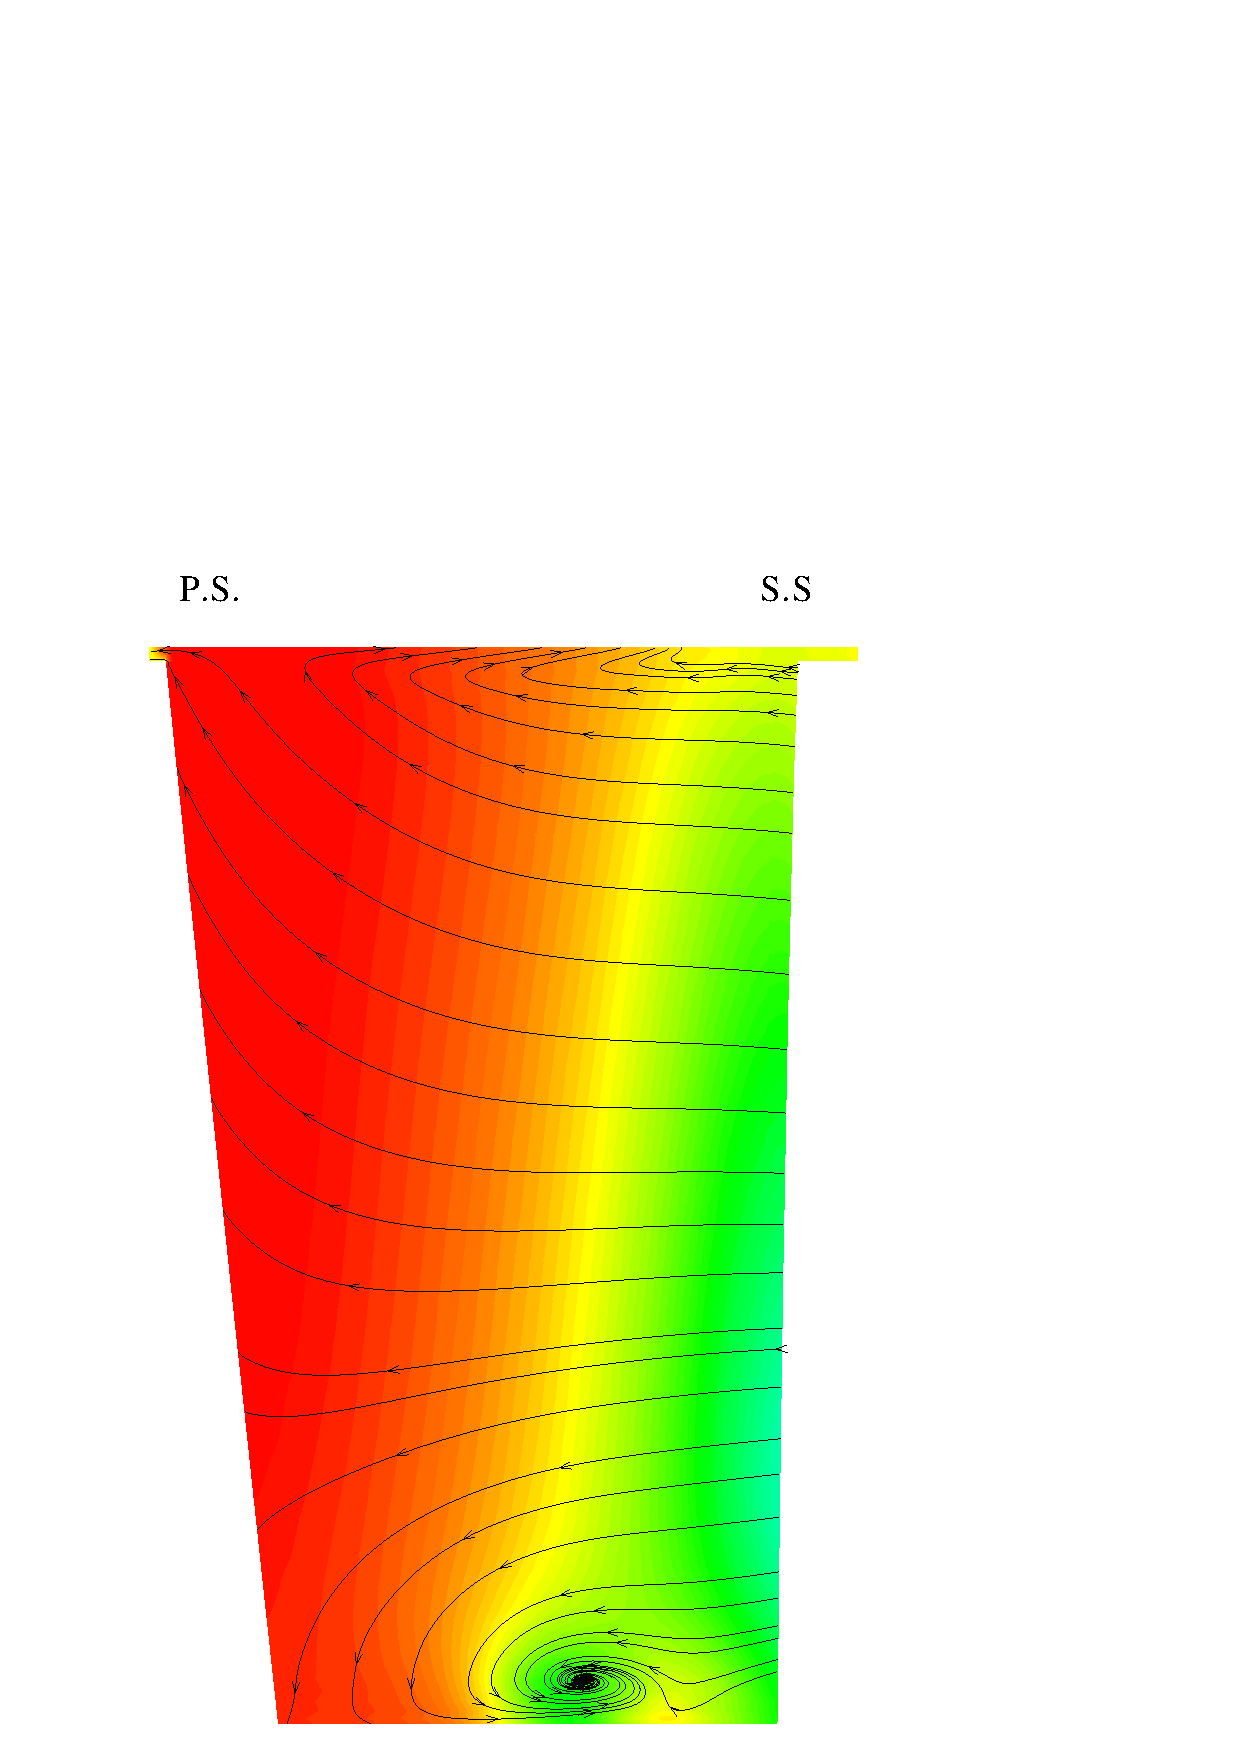
\includegraphics[width=60mm,clip=t]{CHAP_RT27/FIGURE/slid056.pdf}}
        &
    \subfigure[$30\%$ axial chord]
       {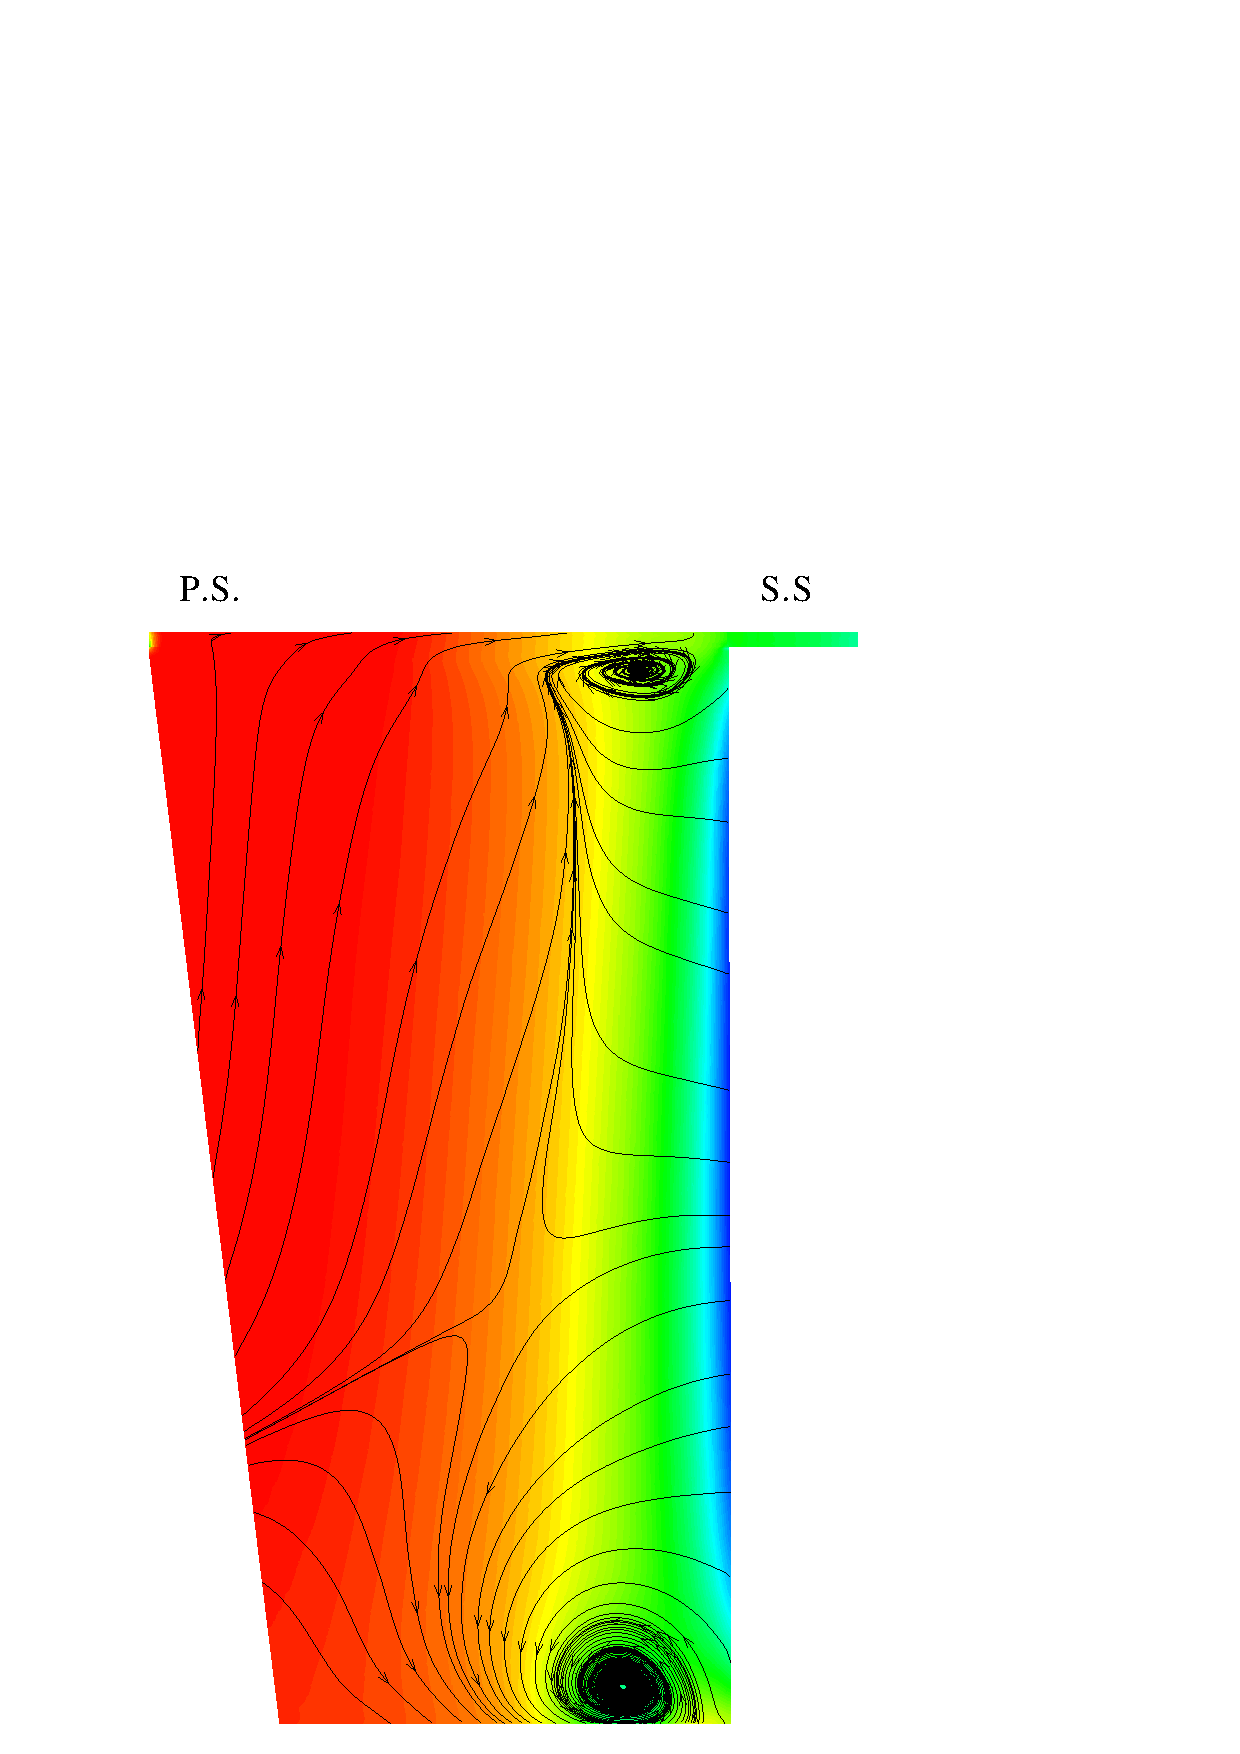
\includegraphics[width=60mm,clip=t]{CHAP_RT27/FIGURE/slid060.pdf}}
        &
    \subfigure
       {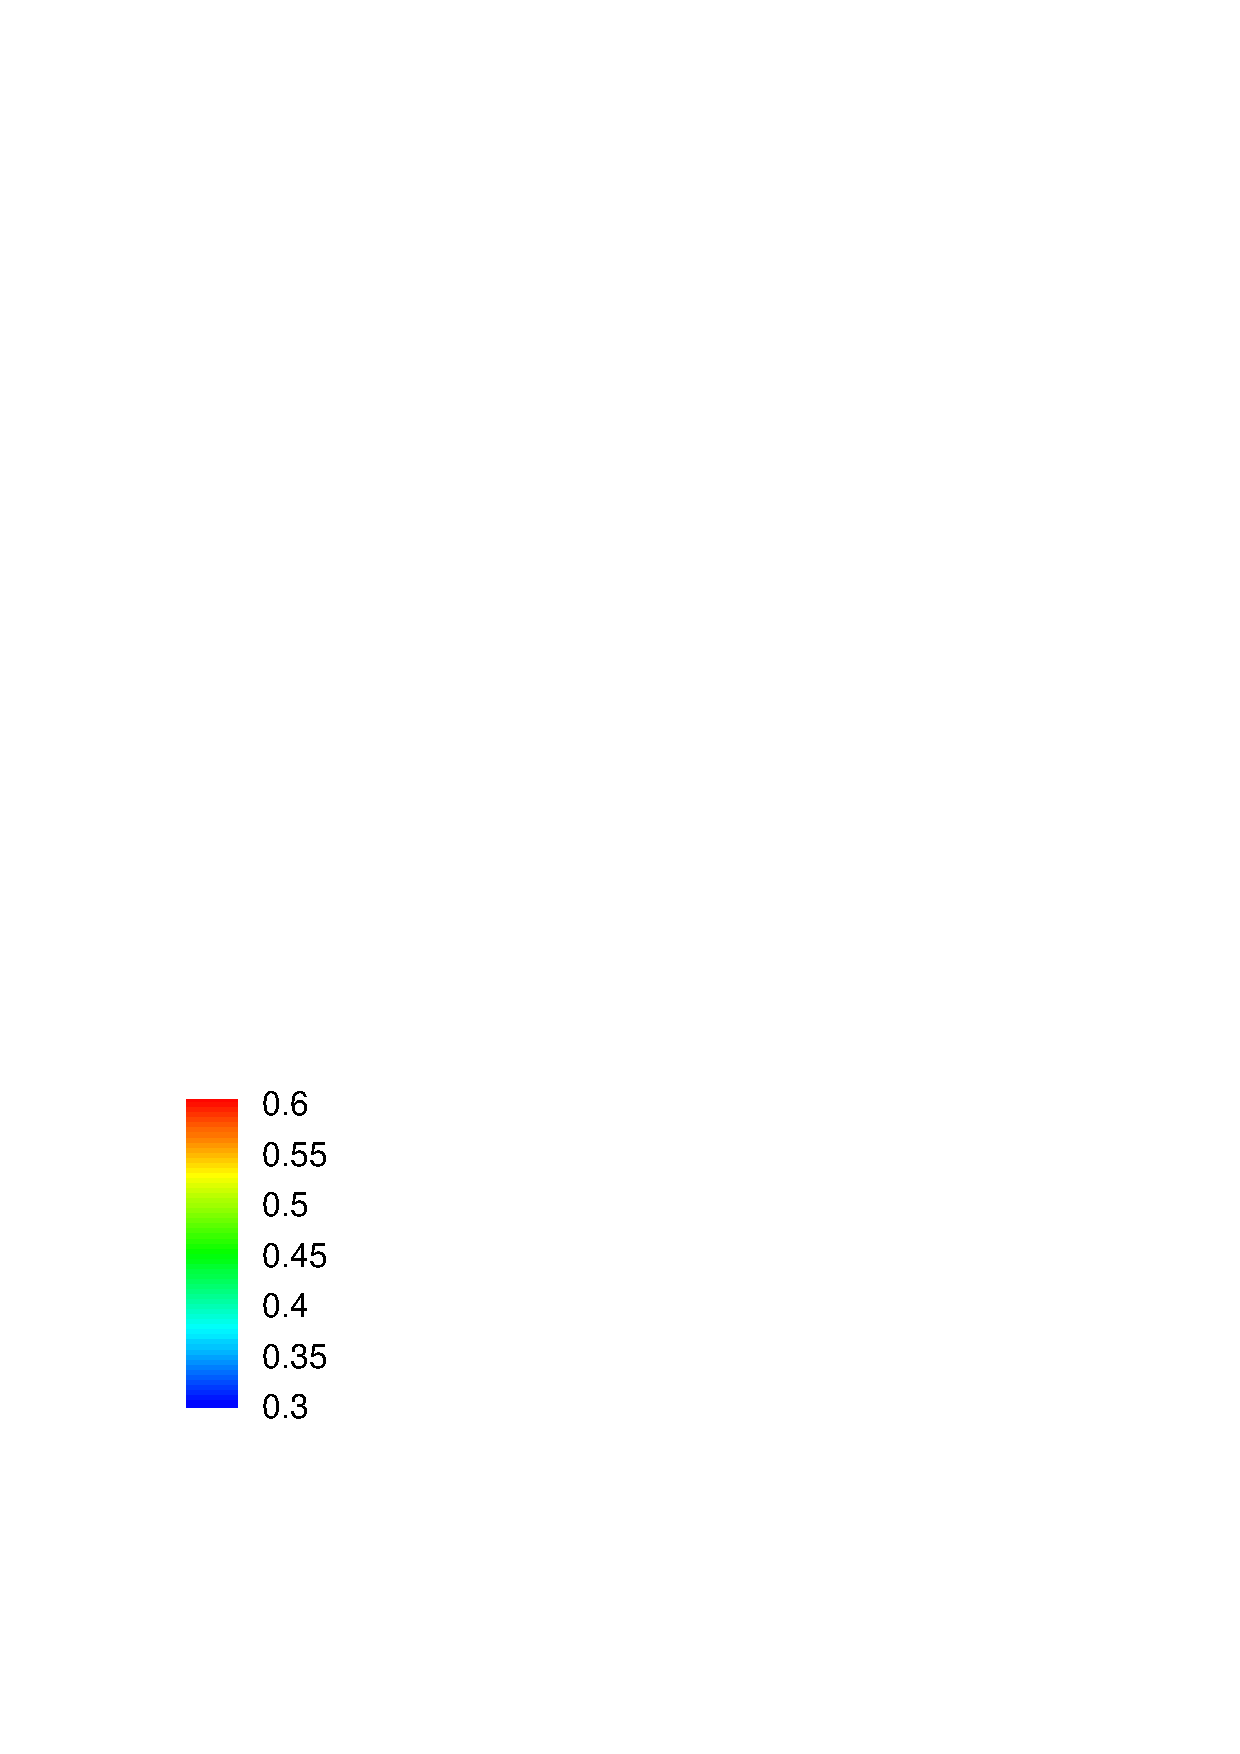
\includegraphics[width=20mm,clip=t]{CHAP_RT27/FIGURE/slid0pr.pdf}}
  \end{tabular}
 \end{center}
 \vspace{-8mm}
 \caption{Pressure contours $\frac{p}{p\sm{01}}$ and particle traces
          at different $r\theta-r$ planes in the RT27a rotor passage}
 \label{rotor_passage_traces.fig}
\end{figure}
%
 The formation of the passage vortex is a natural consequence
 of the interaction between the shear flow at the end wall and
 the turning of the blade.
 The mainstream flow sets up a pressure gradient across the blade
 passage, from the suction to the pressure surfaces, which
 can be approximated by the following relationship:

%
\beq
  \fpd{p}{r} = \frac{\rho u\sm{r}\se{2}}{r}
  \label{equil_radial.eq}
\eeq
%
 where $r$ is the local radius of the turning of the flow caused
 by the blade passage.
 The slower moving boundary layer fluid is subjected to this same
 pressure gradients, but since the velocity $u\sm{r}$ in the boundary layer is
 smaller than the mainstream one, the radius of curvature $r$
 must be smaller.
 Thus in a 3D blade row, the flow on the end wall is
 directed from pressure to suction surface as shown in Fig. \ref{rotor_hub_traces.fig},
 and to preserve continuity, there is a back flow further away from the
 end wall, leading to the vortical flow shown in
 Fig. \ref{rotor_passage_traces.fig}.

 ~\newline
 The flow at the tip is somewhat more complicated. The orifice formed by the
 tip gap experiences essentially the same pressure difference as that
 across the blade.
 Fig. \ref{rotor_tip_traces.fig} shows the static pressure contours as well as
 the particle traces for a radial section inside the tip-gap.
%
\begin{figure}
 \centerline{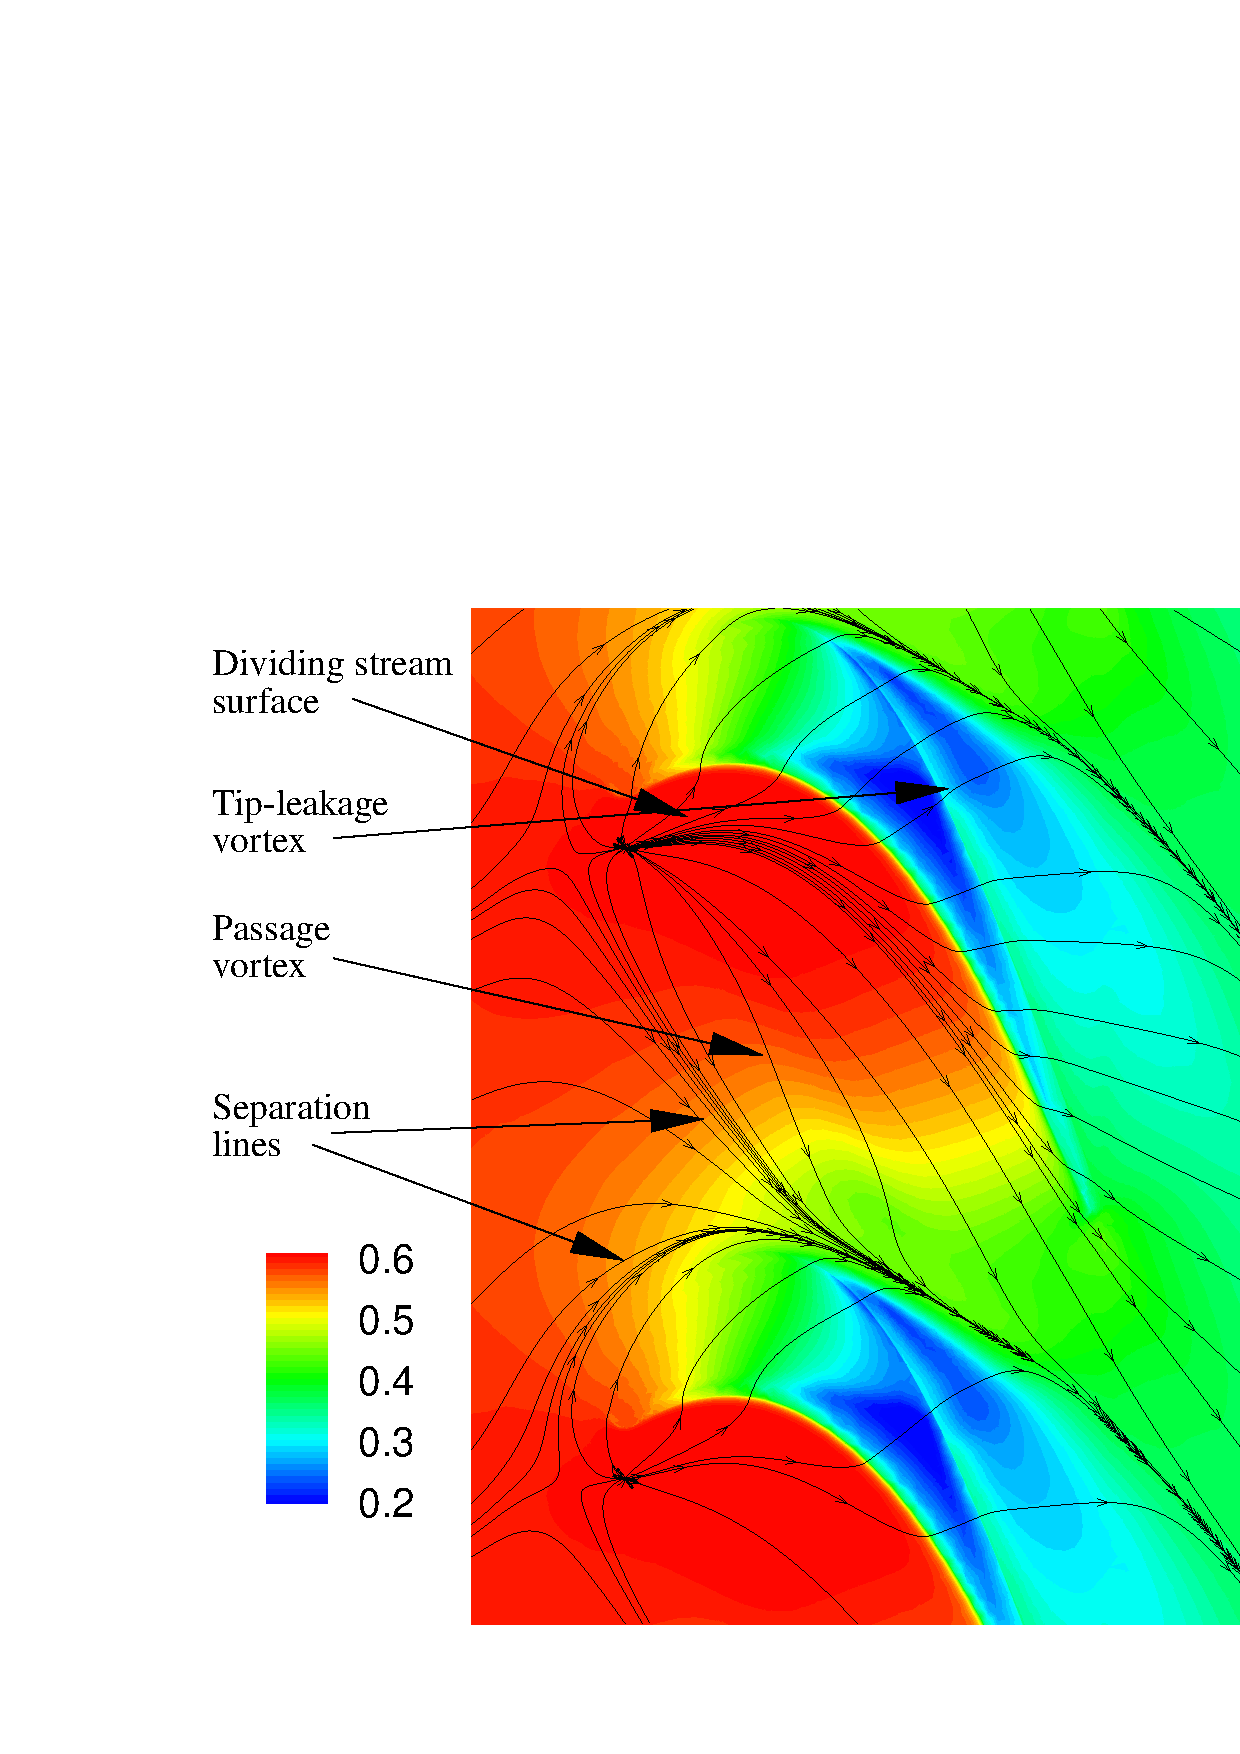
\includegraphics[width=100mm]{CHAP_RT27/FIGURE/rotor_tip_traces.pdf}}
 \caption{Steady state pressure contours $\frac{p}{p\sm{01}}$
          and particle traces inside the RT27a rotor tip-gap region}
 \label{rotor_tip_traces.fig}
\end{figure}
%
 This pressure ratio across the gap accelerates the flow up to supersonic
 conditions. The clearance flow then emerges from the gap with very high velocity
 at an oblique angle relative to the passage flow. The resulting strong interaction
 with the passage flow, including the developing passage vortex of
 Fig. \ref{rotor_tip_traces.fig}, causes the leakage flow to roll up into a vortex
 known as tip-leakage vortex. Such a vortex results in a structure which has a
 vorticity in direction to that of the passage vortex.
 Yamamoto \citeyear{Yamamoto:1} investigated the interaction mechanism
 between tip leakage flow and the passage vortex in some detail.
 At the trailing-edge, the leakage flow pushes the passage vortex away from
 the suction surface, a feature that is evident from Fig. \ref{rotor_tip_traces.fig}.
 Also Yamamoto \citeyear{Yamamoto:1} suggests that the interaction between the
 two vortex structures results in an elongation and distortion of the passage vortex.
 In particular, the leakage flow pushes the secondary flow towards midspan.
 This seems to be in an agreement with what is shown in
 Fig. \ref{rotor_blade_traces.fig}.

 Another important feature of the tip-clearance flow
 is the formation of a dividing stream surface between the fluid which is swept
 into the gap and that which is driven across the passage in the usual way.
 Such a stream surface is evident in Fig. \ref{rotor_tip_traces.fig}
 where it lies at about one fifth of the blade pitch from the pressure
 surface. The exact position of the division stream surface is a function
 of the clearance and probably other parameters such as the blade loading
 (Sjolander \& Amrud \citeyearNP{Sjolander:1}).

 Fig. \ref{rotor_tip_traces.fig} also shows the absence of the
 stagnation point due to the presence of the clearance.
 On the other hand, the two separation lines of the horseshoe
 vortex are still present.
 For larger clearances, Sjolander \& Amrud \citeyear{Sjolander:1} show
 that the tip horseshoe vortex disappears.
%
%
%

%
%
%
%
%
\section{Rotor Unsteady Flow Analysis}
\label{rt27_unsteady.sec}
\headb{Transonic Turbine Stage}{Rotor unsteady flow analysis}
%
%
 In this section unsteady results obtained using the linear
 frequency domain approach are presented. First, the sources of unsteadiness
 obtained from the NGV outlet steady-state solution are discussed.
 Potential- and vortical-rotor interactions were evaluated for the first
 two tangential Fourier modes and the superimposed results
 compared with the available experimental data.
 Sections \ref{rt27_vortical.subsec} and \ref{rt27_potential.subsec}
 present a physical interpretation of the two type unsteady interactions, i.e.
 potential and vortical.
 As reported in Appendix \ref{waves.chap}, there is a third type of unsteady
 interaction caused by the entropy variation across the NGV wake. This interaction
 produces unsteady pressure variations which are of one order of magnitude
 less then those obtained from the potential and vortical NGV non-uniformities.
 For this reason the entropy mode is included in the vortical mode, also associated
 with the NGV-wake.
 This means that the total unsteady flow-filed in the rotor passage is given by the
 superimposition of the potential and vortical modes.
%
%
%
%
\subsection{Sources of unsteadiness}
\label{rt27_sources.subsec}
%
%
 The sources of unsteadiness in the rotor passage are represented by the
 steady-state tangential non-uniformities at the outflow boundaries
 of the stator blade.
 Such non-uniformities, which can be assumed to
 be approximately steady in the stator frame of reference, are unsteady
 in the rotor frame of reference since the rotor is moving
 through them.
%
%
\begin{figure}
 \begin{center}
  \begin{tabular}{c}
    \subfigure[Dimensionless static pressure]
       {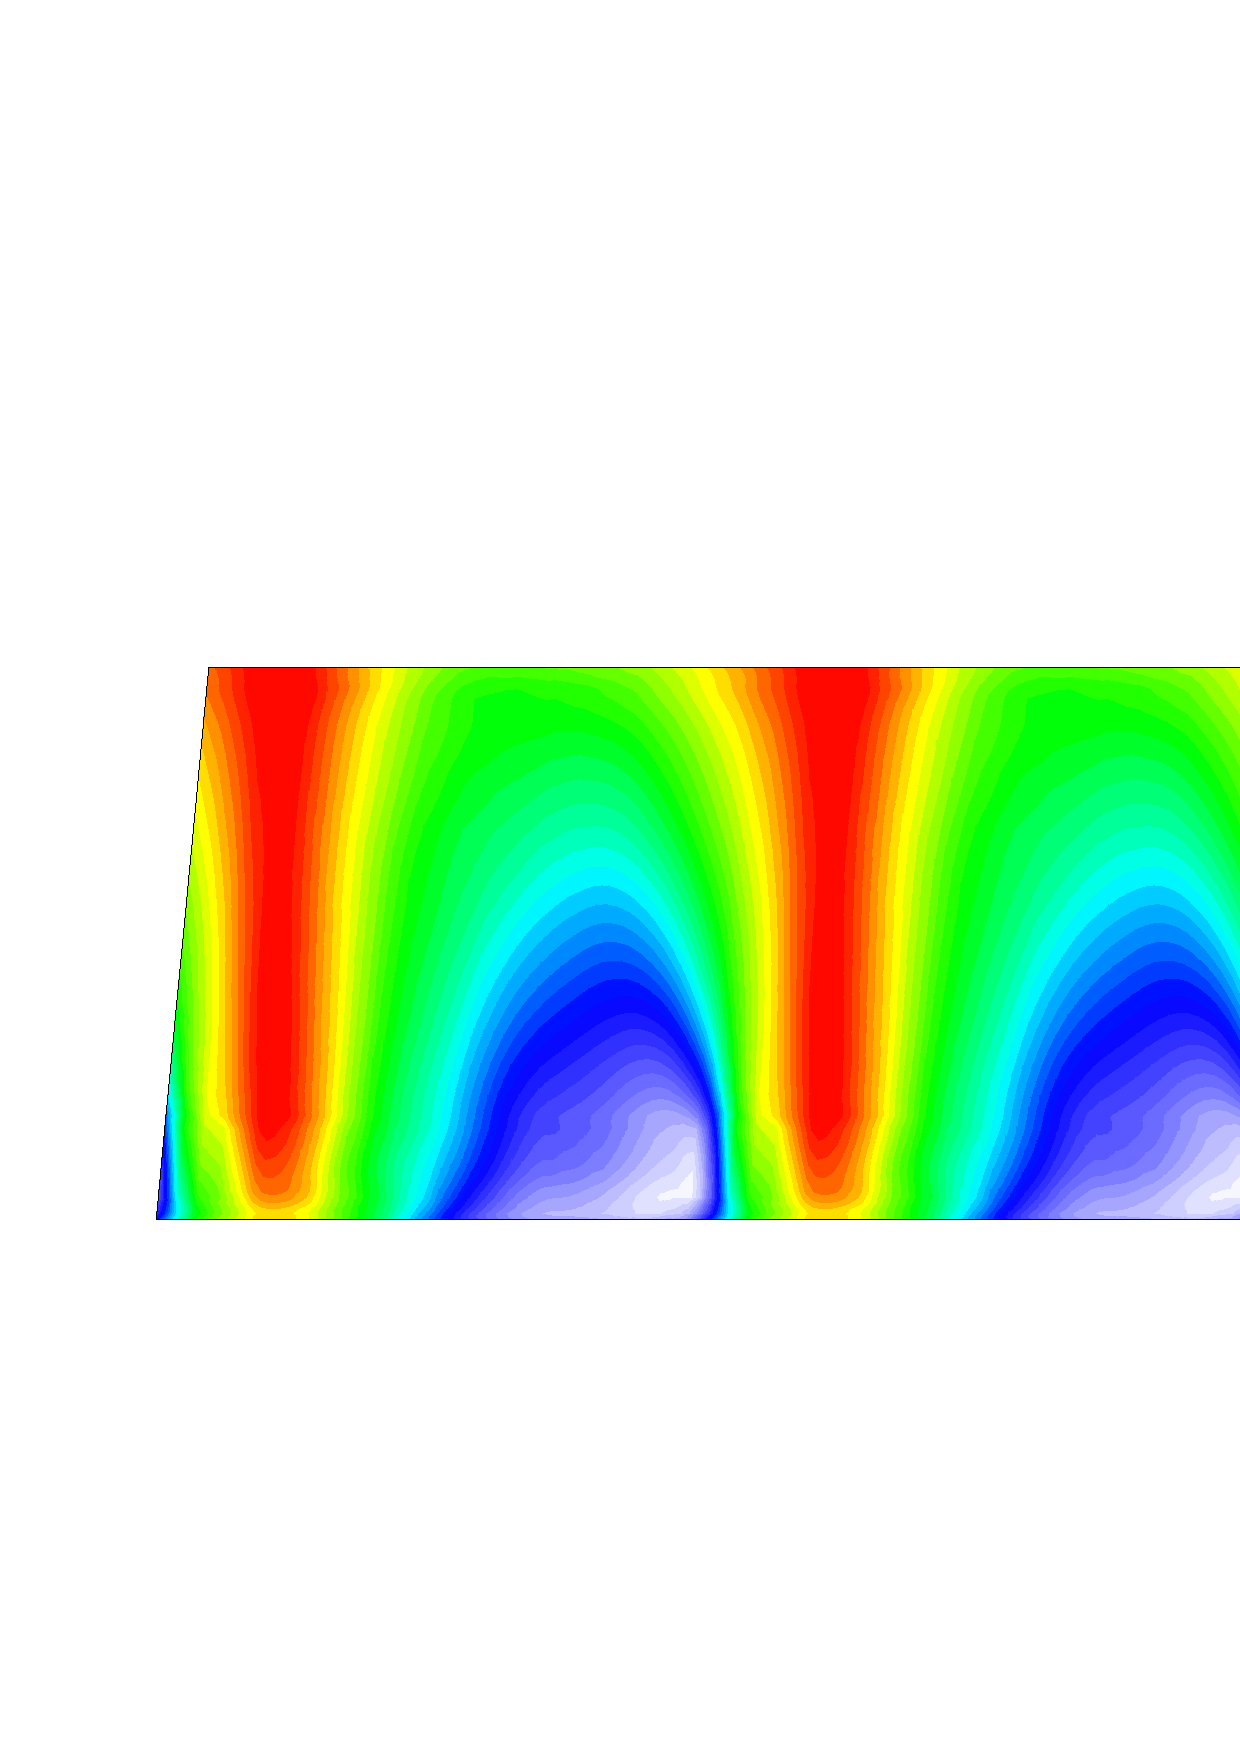
\includegraphics[width=130mm,clip=t]{CHAP_RT27/FIGURE/ngvout_pres.pdf}}
      \vspace{-2mm}\\
    \subfigure[Mach number]
       {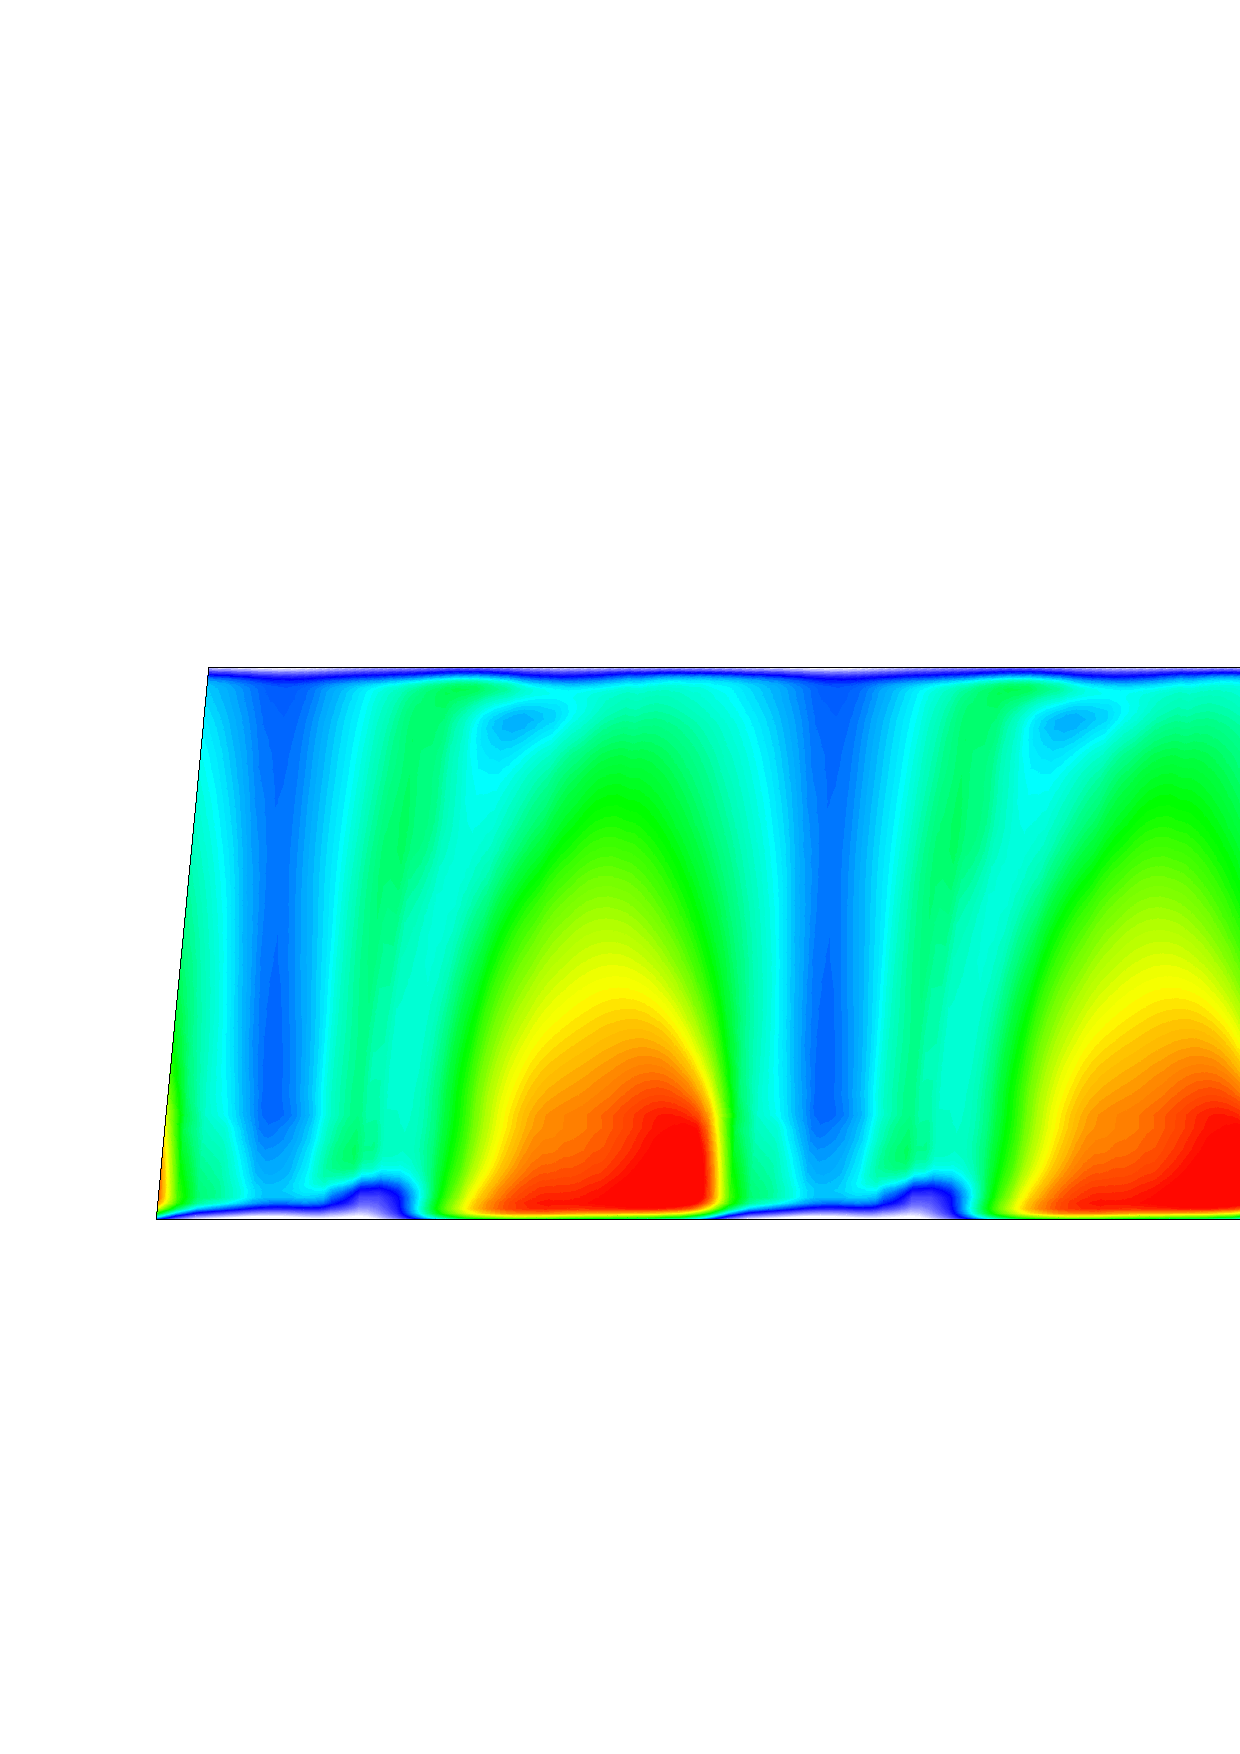
\includegraphics[width=130mm,clip=t]{CHAP_RT27/FIGURE/ngvout_mach.pdf}}
      \vspace{-2mm}\\
    \subfigure[Dimensionless total pressure]
       {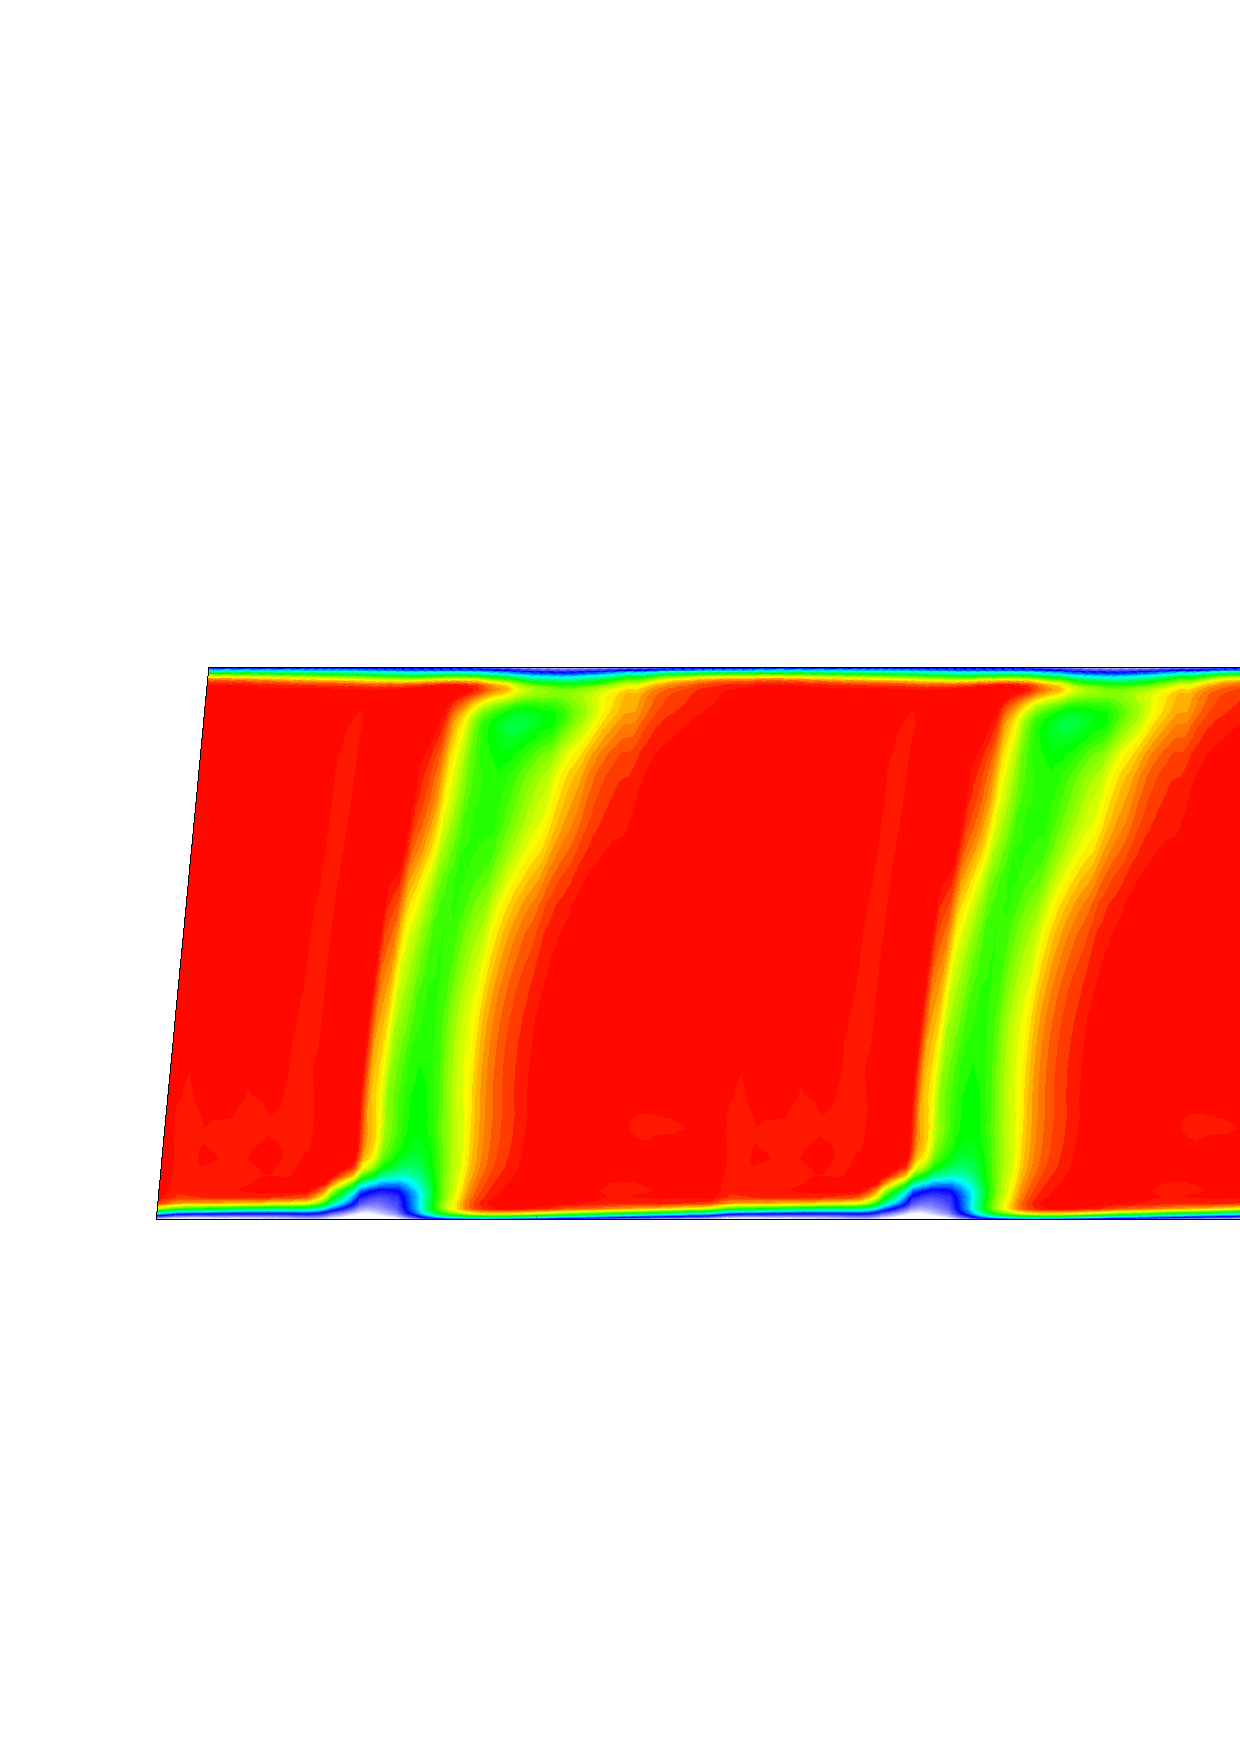
\includegraphics[width=130mm,clip=t]{CHAP_RT27/FIGURE/ngvout_ptot.pdf}}
  \end{tabular}
 \end{center}
 \vspace{-8mm}
 \caption{Steady state solution at the RT27a NGV outlet boundary (2 passages)}
 \label{ngv_outlet_solution.fig}
\end{figure}
%
 Fig. \ref{ngv_outlet_solution.fig} shows the computed steady-state
 solution at the NGV outlet. The static pressure distribution shows a
 weak shock wave towards the hub section where the average outlet Mach number
 is just above unity.
 The Mach number contours in Fig. \ref{ngv_outlet_solution.fig}b
 show the potential field associated with the static pressure contours
 but the wake profile is not evident apart from the hub
 section of the blade where the wake seems to have a quite strong
 radial variation.
 The total pressure contours, on the other hand, clearly exhibit the
 wake structure which appears to run almost radially, with the exception of
 the root region.
%
\begin{figure}
 \begin{center}
  \begin{tabular}{c}
    \subfigure[Vortical component of dimensionless absolute velocity]
        {\begin{tabular}{cc}
        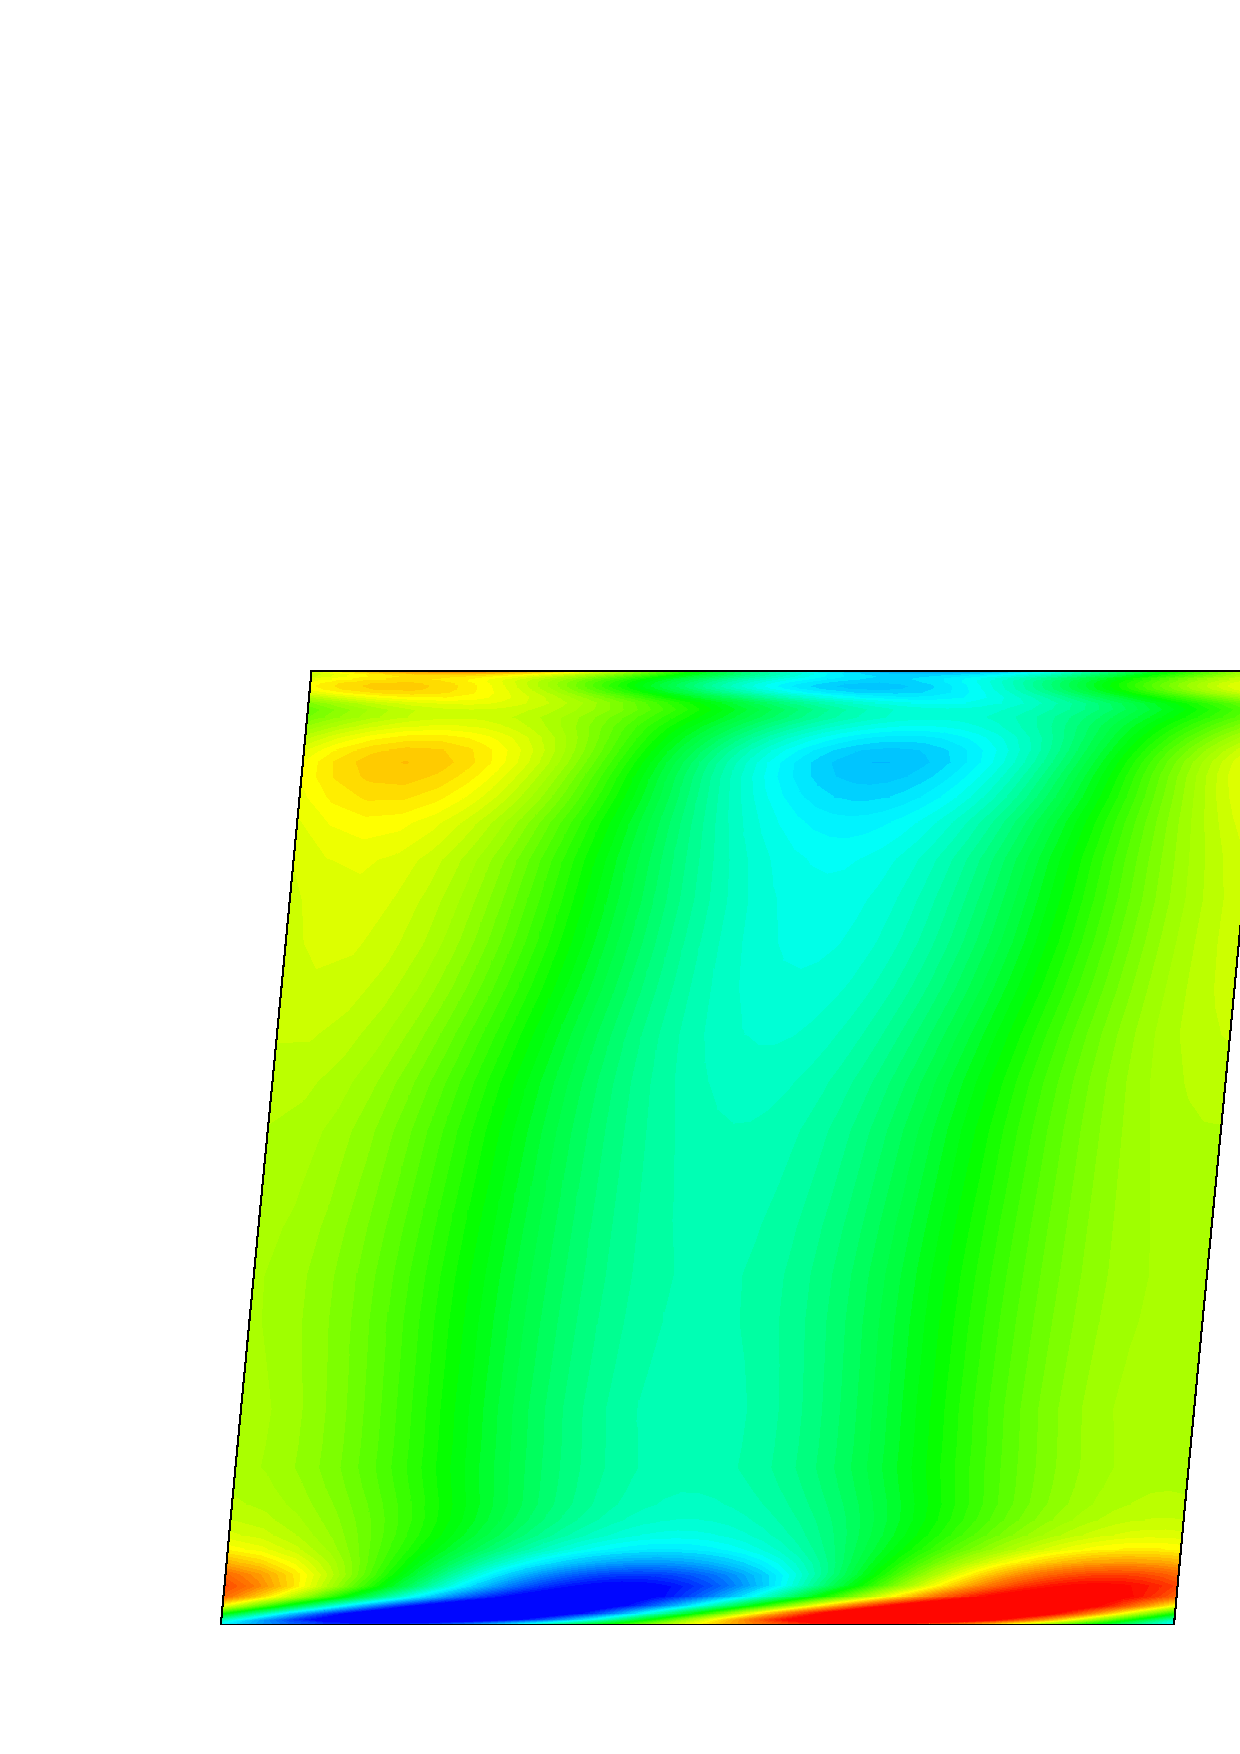
\includegraphics[width=70mm,clip=t]{CHAP_RT27/FIGURE/out_vort1.pdf}
        &
        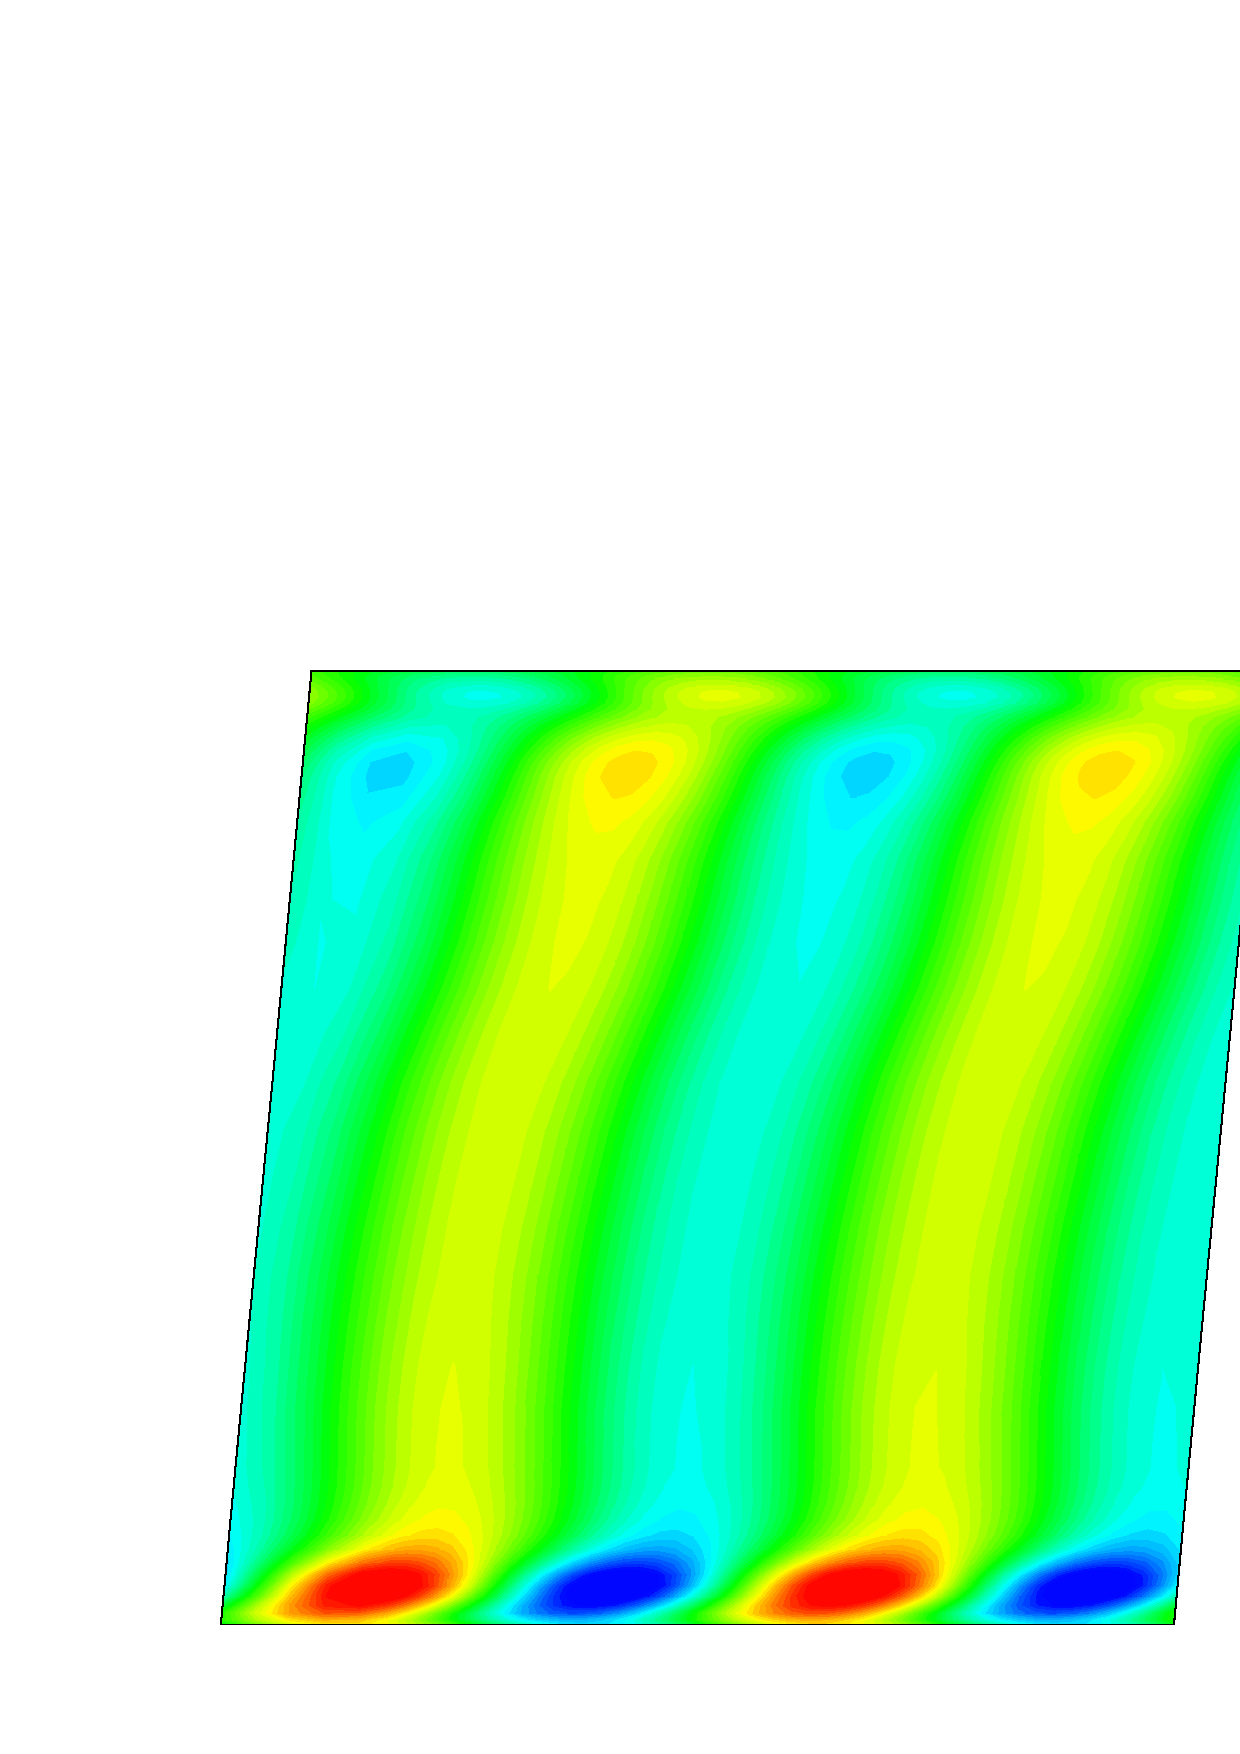
\includegraphics[width=70mm,clip=t]{CHAP_RT27/FIGURE/out_vort2.pdf}
        \end{tabular}}
    \vspace{-2mm}\\
    \subfigure[Dimensionless pressure]
        {\begin{tabular}{cc}
        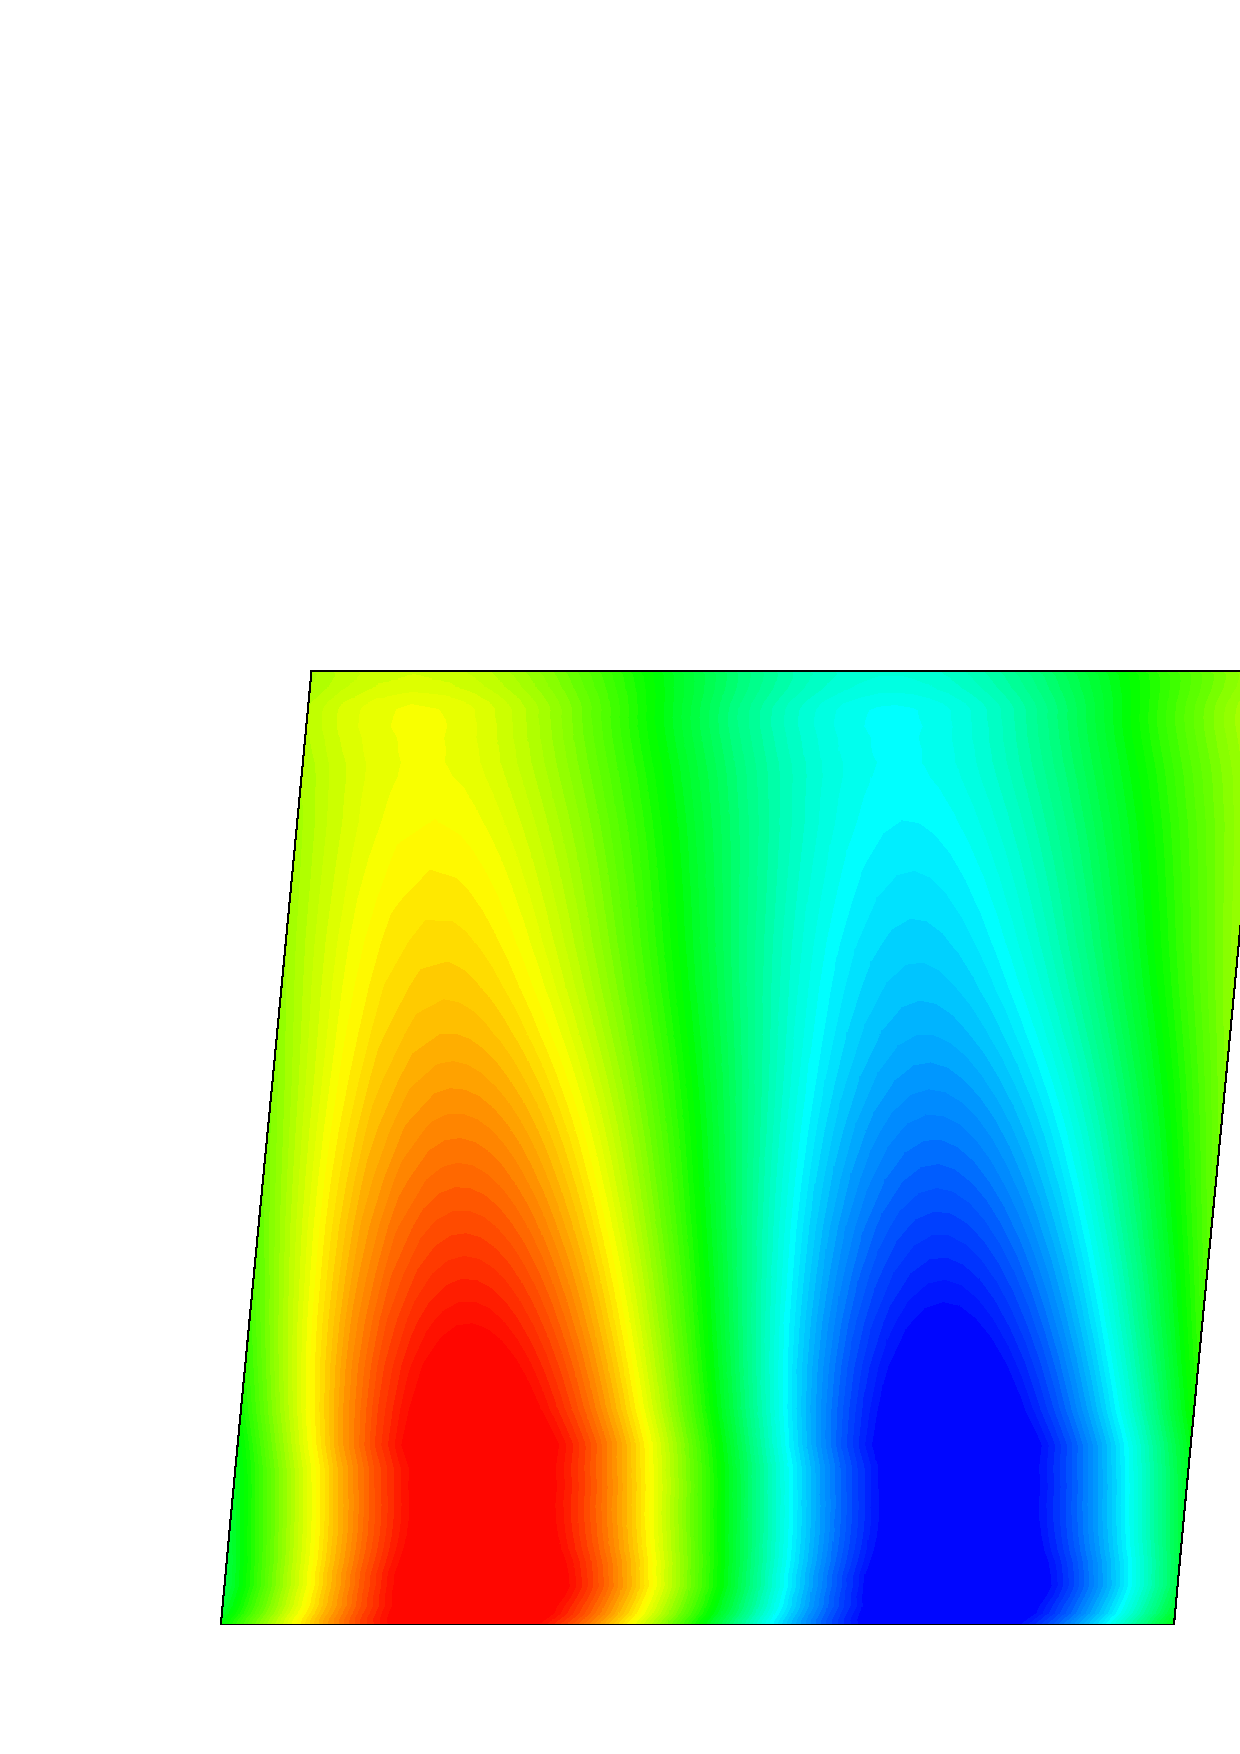
\includegraphics[width=70mm,clip=t]{CHAP_RT27/FIGURE/out_pote1.pdf}
        &
        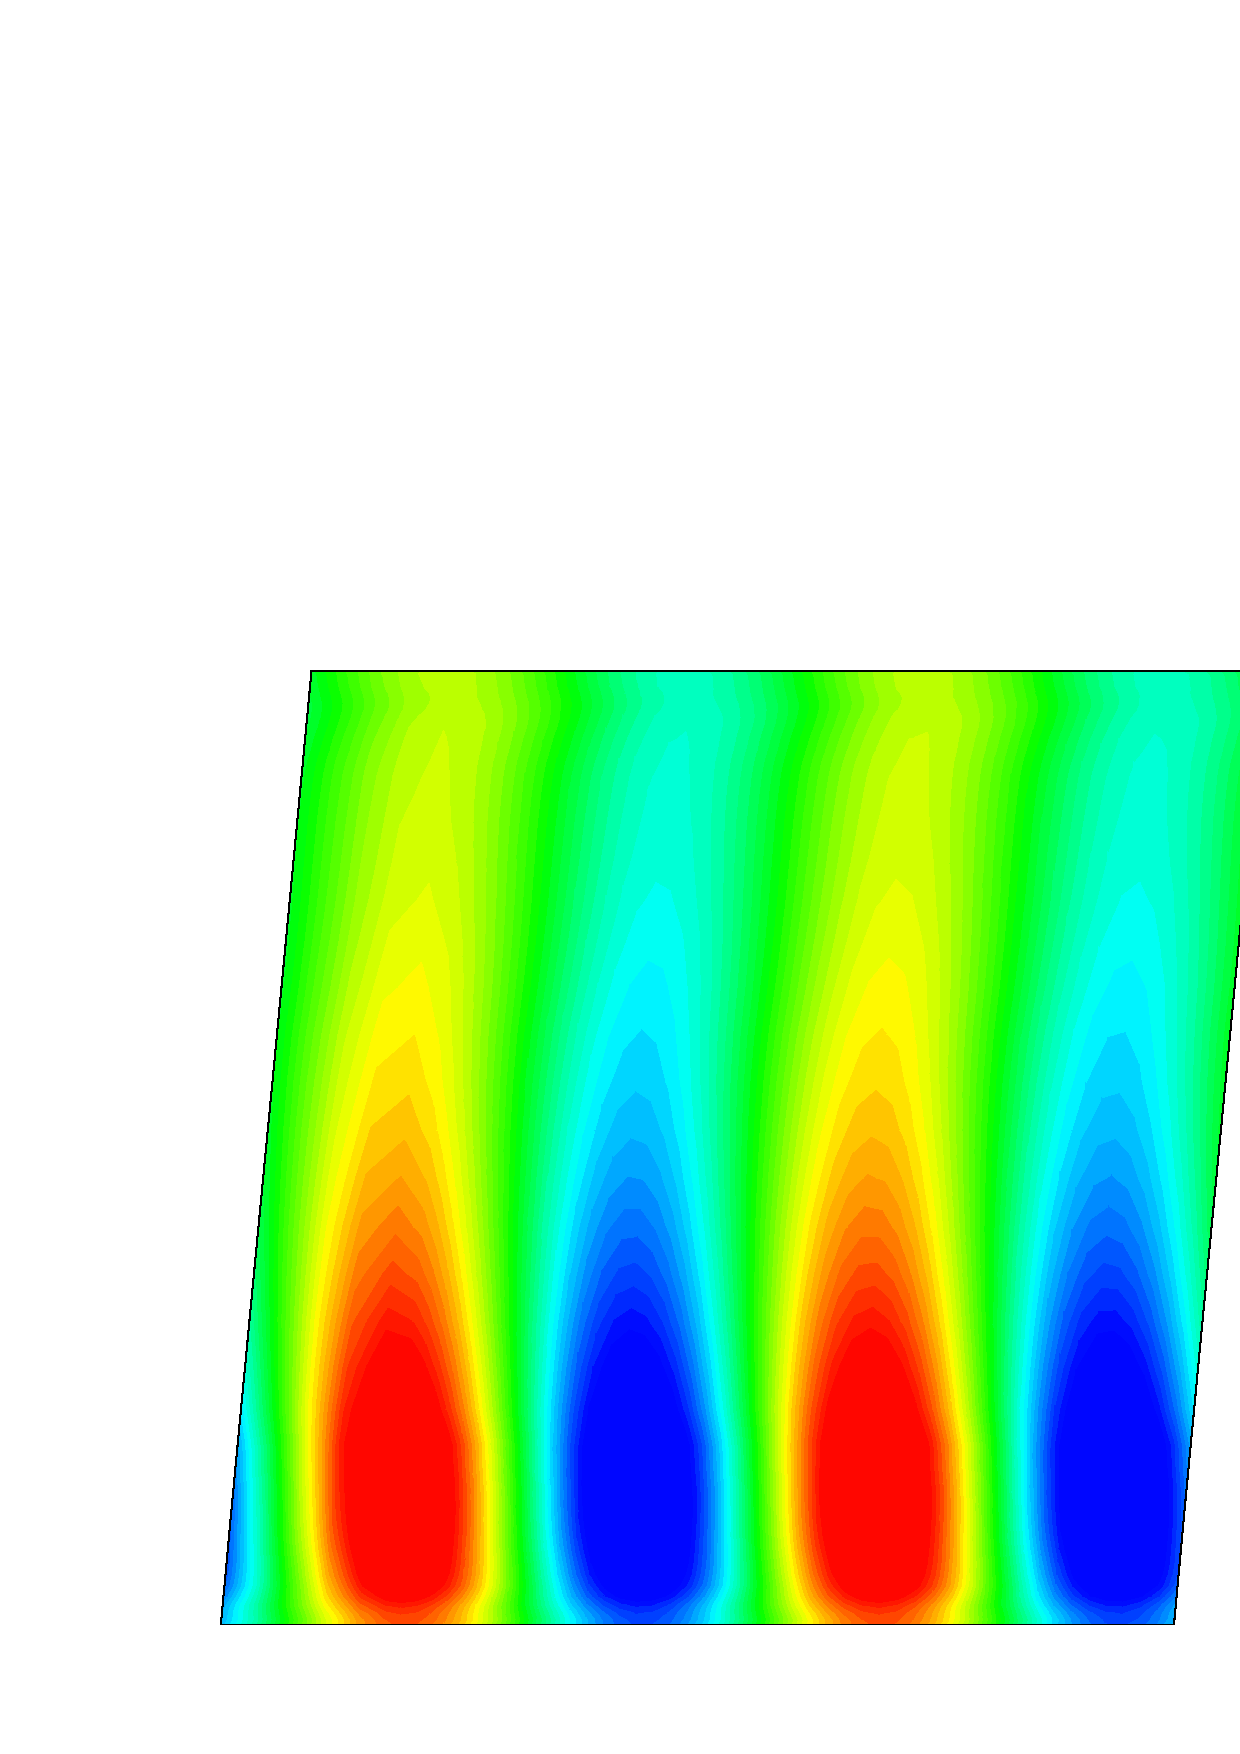
\includegraphics[width=70mm,clip=t]{CHAP_RT27/FIGURE/out_pote2.pdf}
        \end{tabular}}
    \vspace{-2mm}\\
    \subfigure[Entropic component of dimensionless density]
        {\begin{tabular}{cc}
        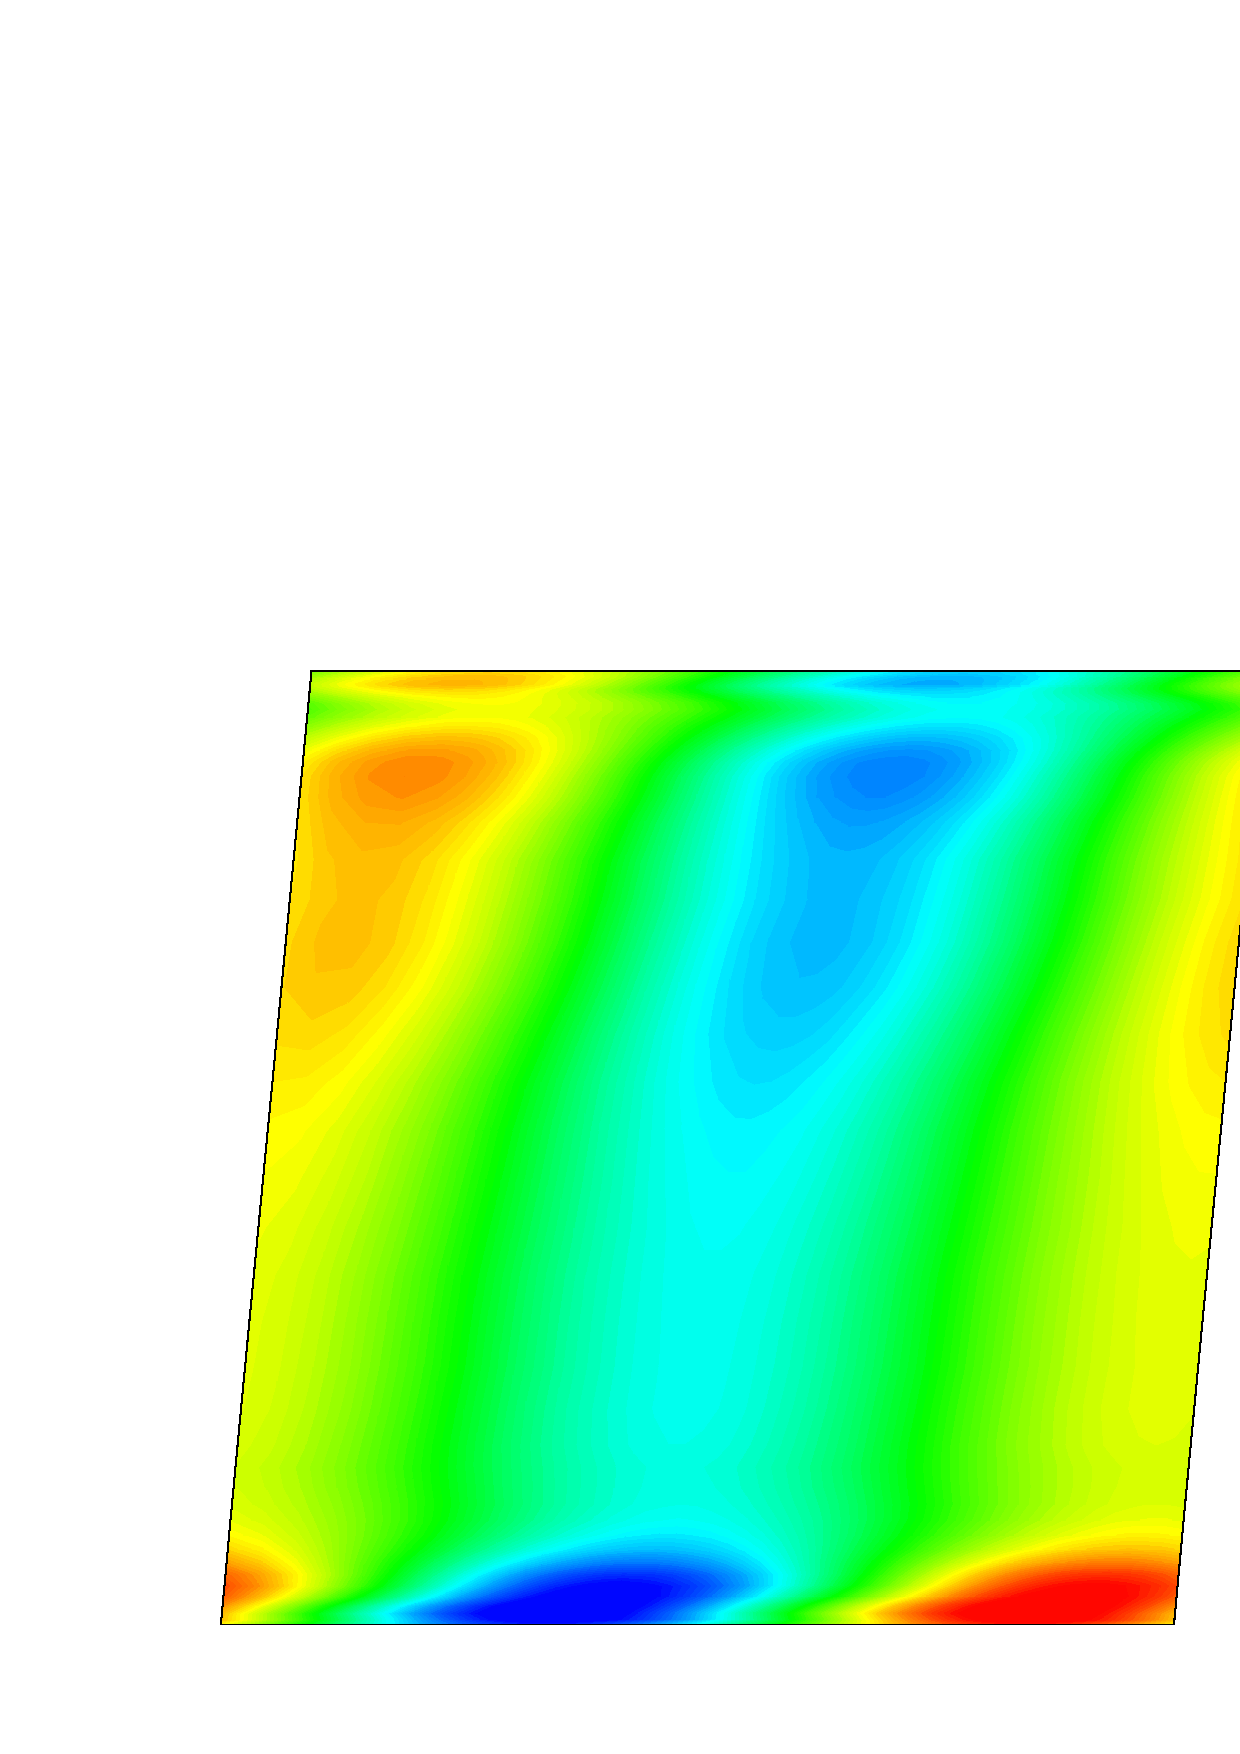
\includegraphics[width=70mm,clip=t]{CHAP_RT27/FIGURE/out_entr1.pdf}
        &
        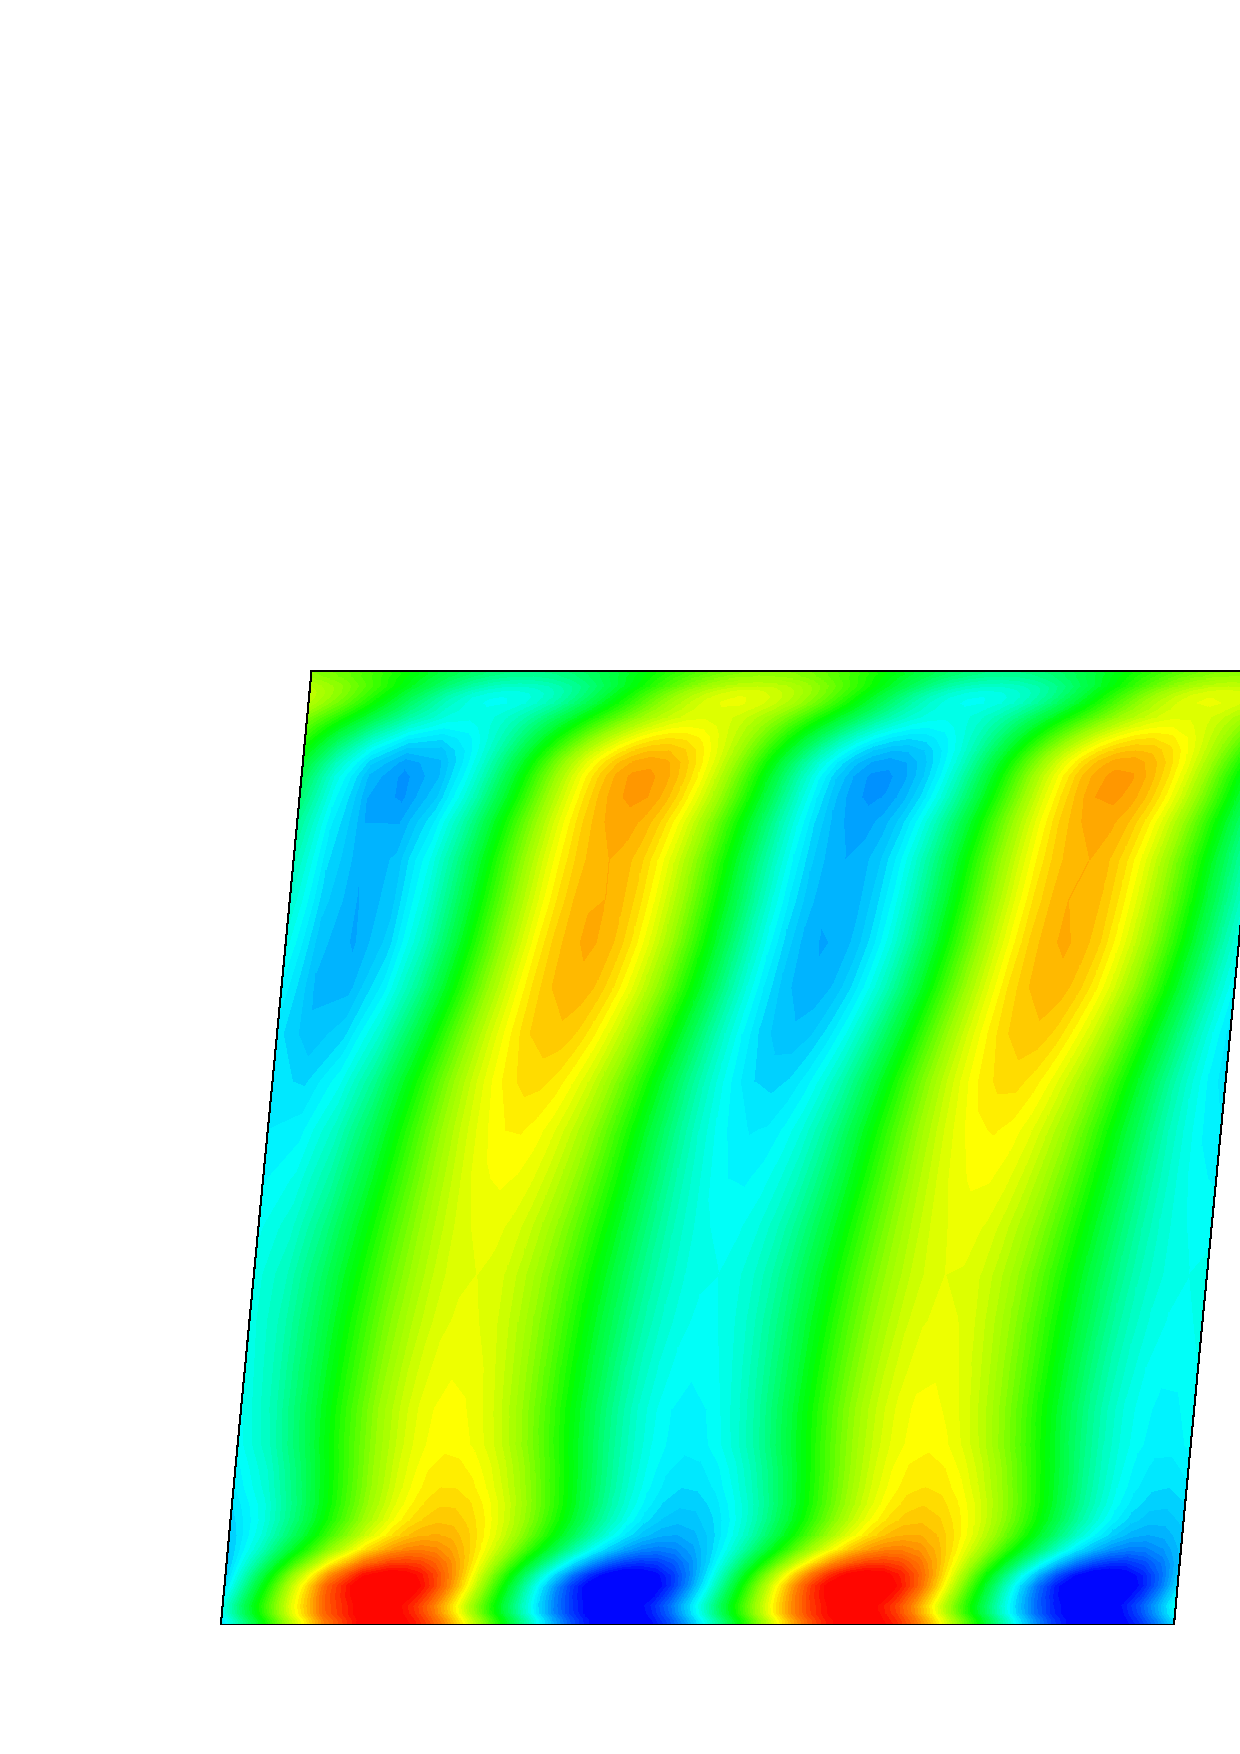
\includegraphics[width=70mm,clip=t]{CHAP_RT27/FIGURE/out_entr2.pdf}
        \end{tabular}}
    \end{tabular}
 \end{center}
 \vspace{-8mm}
 \caption{First (left) and second (right) Fourier components
          of spatial non-uniformities of RT27a NGV outlet solution (1 passage)}
 \label{ngv_outlet_decomposed1.fig}
\end{figure}
%
%
%
 The rotor blades move through the steady NGV-outlet from left to right of
 Fig. \ref{ngv_outlet_solution.fig} and they see the spatial non-uniformities
 as unsteady perturbations.
 Such spatial non-uniformities are periodic in the tangential coordinate
 and they can be decomposed into Fourier components for each radial section.
 The unsteady velocities contain two parts: a rotational (vortical) part, associated
 with the NGV wake, and an irrotational (potential) part associated with pressure
 variations. In the same way, the unsteady density contains two parts: an entropic
 part associated with the NGV wake and an irrotational (potential) part, again
 associated with the pressure variation.
 Such a grouping means that each Fourier mode of the steady flow solution at the
 NGV outlet can be seen as summation of three different modes:
 vortical, potential and entropic.
 Appendix \ref{waves.chap} shows how to calculate
 such modes for each Fourier harmonic using Goldstein's splitting theorem
 and the linearised acoustic equations.

 The vortical component of the spatial non-uniformities is associated with
 velocity variations with zero divergence and hence with
 the velocity defect in the NGV wake.
 Fig. \ref{ngv_outlet_decomposed1.fig}a shows the first two Fourier components
 of the absolute velocity variations associated with the vortical component.
 The first harmonic, usually referred as `gust'
 (Manwaring \& Wisler \citeyearNP{Manwaring:1}), clearly shows the
 three-dimensionality of the NGV-wake towards the root section. Very large
 velocity deficit occurs half a cycle or so earlier that the
 mid-height wake. Such wake inclination was also measured by Moss et al.
 \citeyear{Moss:1}.
 Fig. \ref{ngv_outlet_decomposed1.fig}b shows the pressure perturbation
 which is associated only with the potential field of the NGV outlet.
 Neither Fourier component has strong 3D features.
 The first two harmonics of the density perturbation associated with
 the entropic mode are shown in Fig. \ref{ngv_outlet_decomposed1.fig}c.
%
%
%
\begin{figure}
 \begin{center}
  \begin{tabular}{cc}
    \subfigure[Vortical component]
       {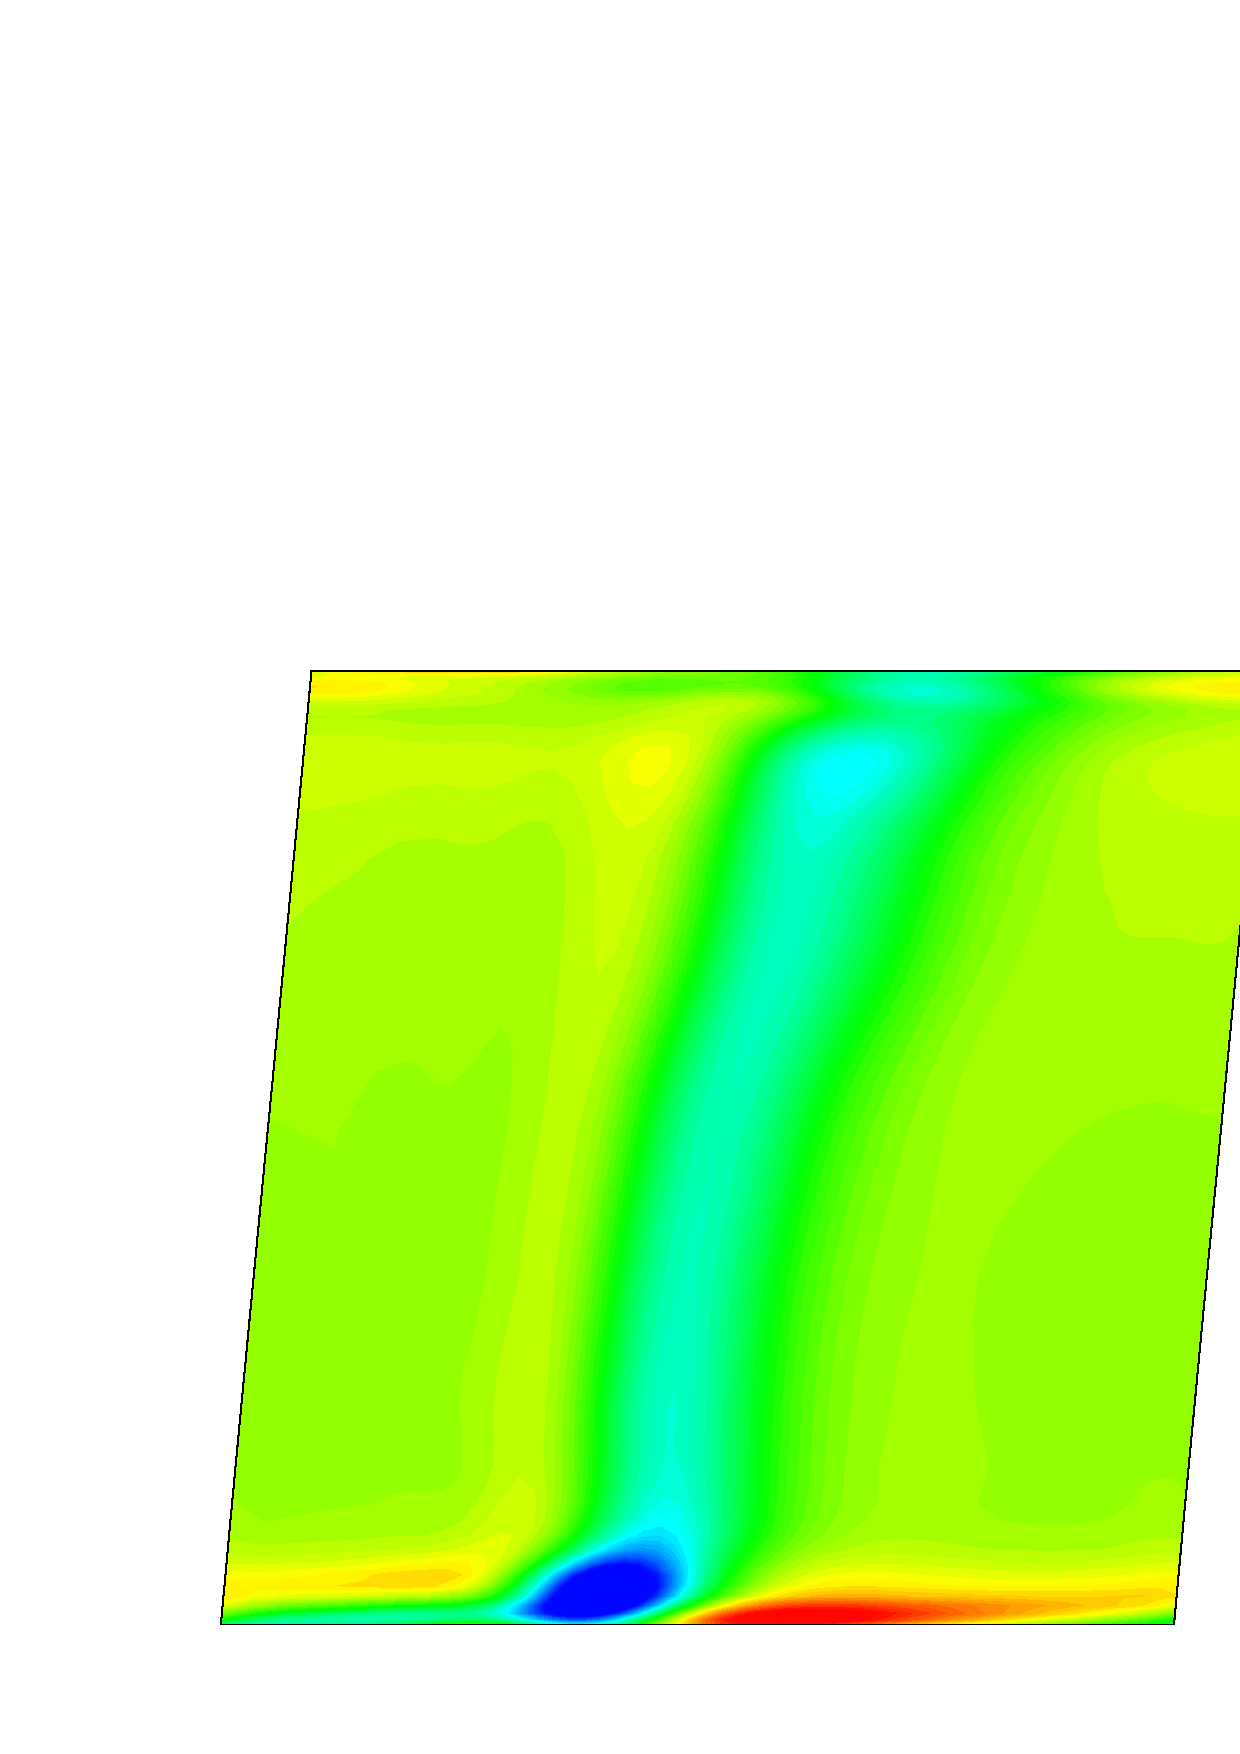
\includegraphics[width=70mm,clip=t]{CHAP_RT27/FIGURE/out_vel_vor.pdf}}
      &
    \subfigure[Potential component]
       {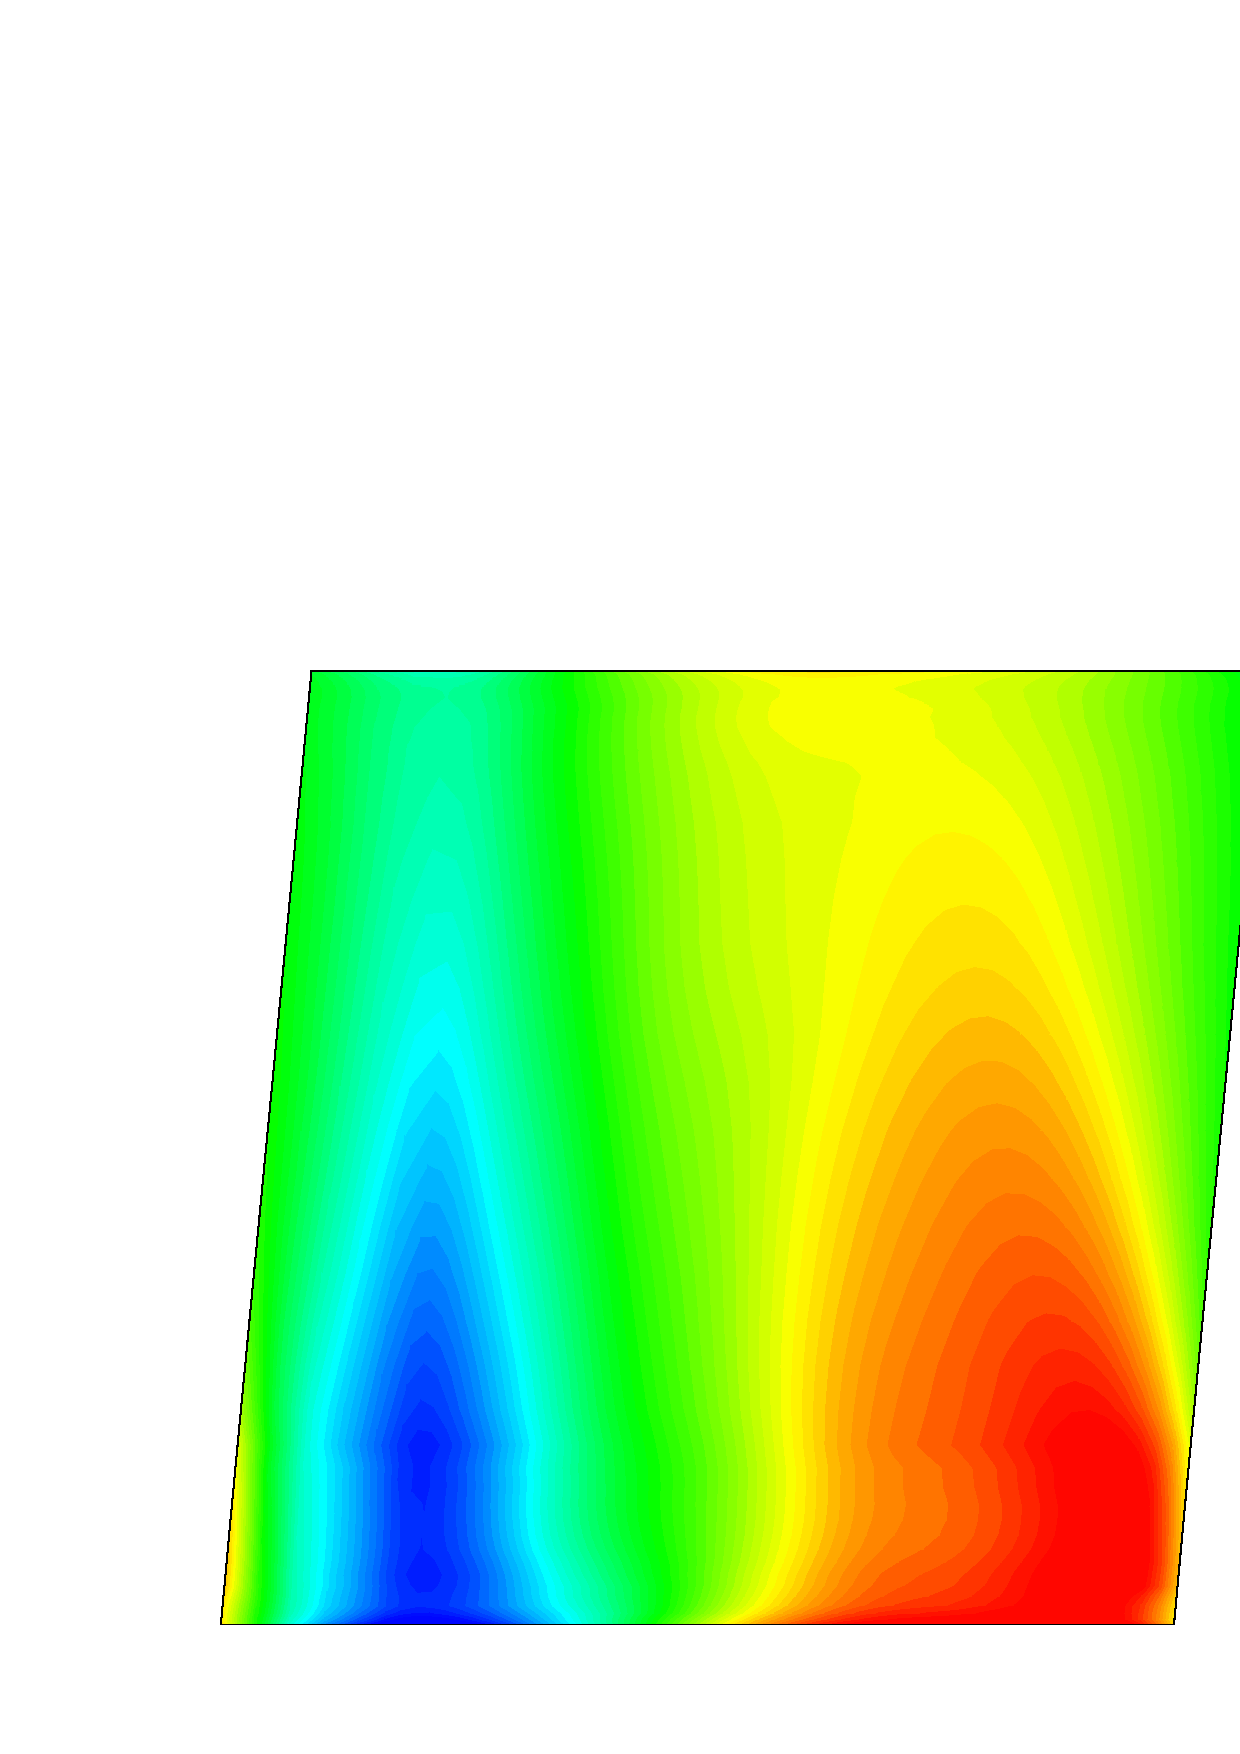
\includegraphics[width=70mm,clip=t]{CHAP_RT27/FIGURE/out_vel_pot.pdf}}
  \end{tabular}
 \end{center}
 \vspace{-8mm}
 \caption{Vortical and potential components of
          dimensionless absolute velocity variation at RT27a NGV outlet
          (reconstructed using first twenty harmonics)}
 \label{ngv_outlet_decomposed2.fig}
\end{figure}
%
 Fig. \ref{ngv_outlet_decomposed2.fig} shows the vortical and potential components
 of the absolute velocity non-uniformities at the NGV outlet. These two plots
 have been obtained by a summation of the first twenty
 vortical and potential Fourier components.
%
%
%
%
%
\subsection{Comparison with measured data}
\label{rt27_comparison.subsec}
%
 The computed unsteady flow results, obtained from the superimposition of
 the potential and vortical calculations, will
 now be compared with the experimental data of Moss et al. \citeyear{Moss:1}.
 The comparison is made for three different span-wise positions, namely
 mid-root, mid-height and tip. The remaining two sections, root
 and mid-tip, are not considered because of the unavailability of
 experimental data for the rotor suction surface.
%
%
\begin{figure}
  \begin{flushleft}
   \begin{tabular}{l}
     \subfigure[Mid-root section ($10\%$ span)]
      {\begin{tabular}{ll}
        \hspace{-5mm}
        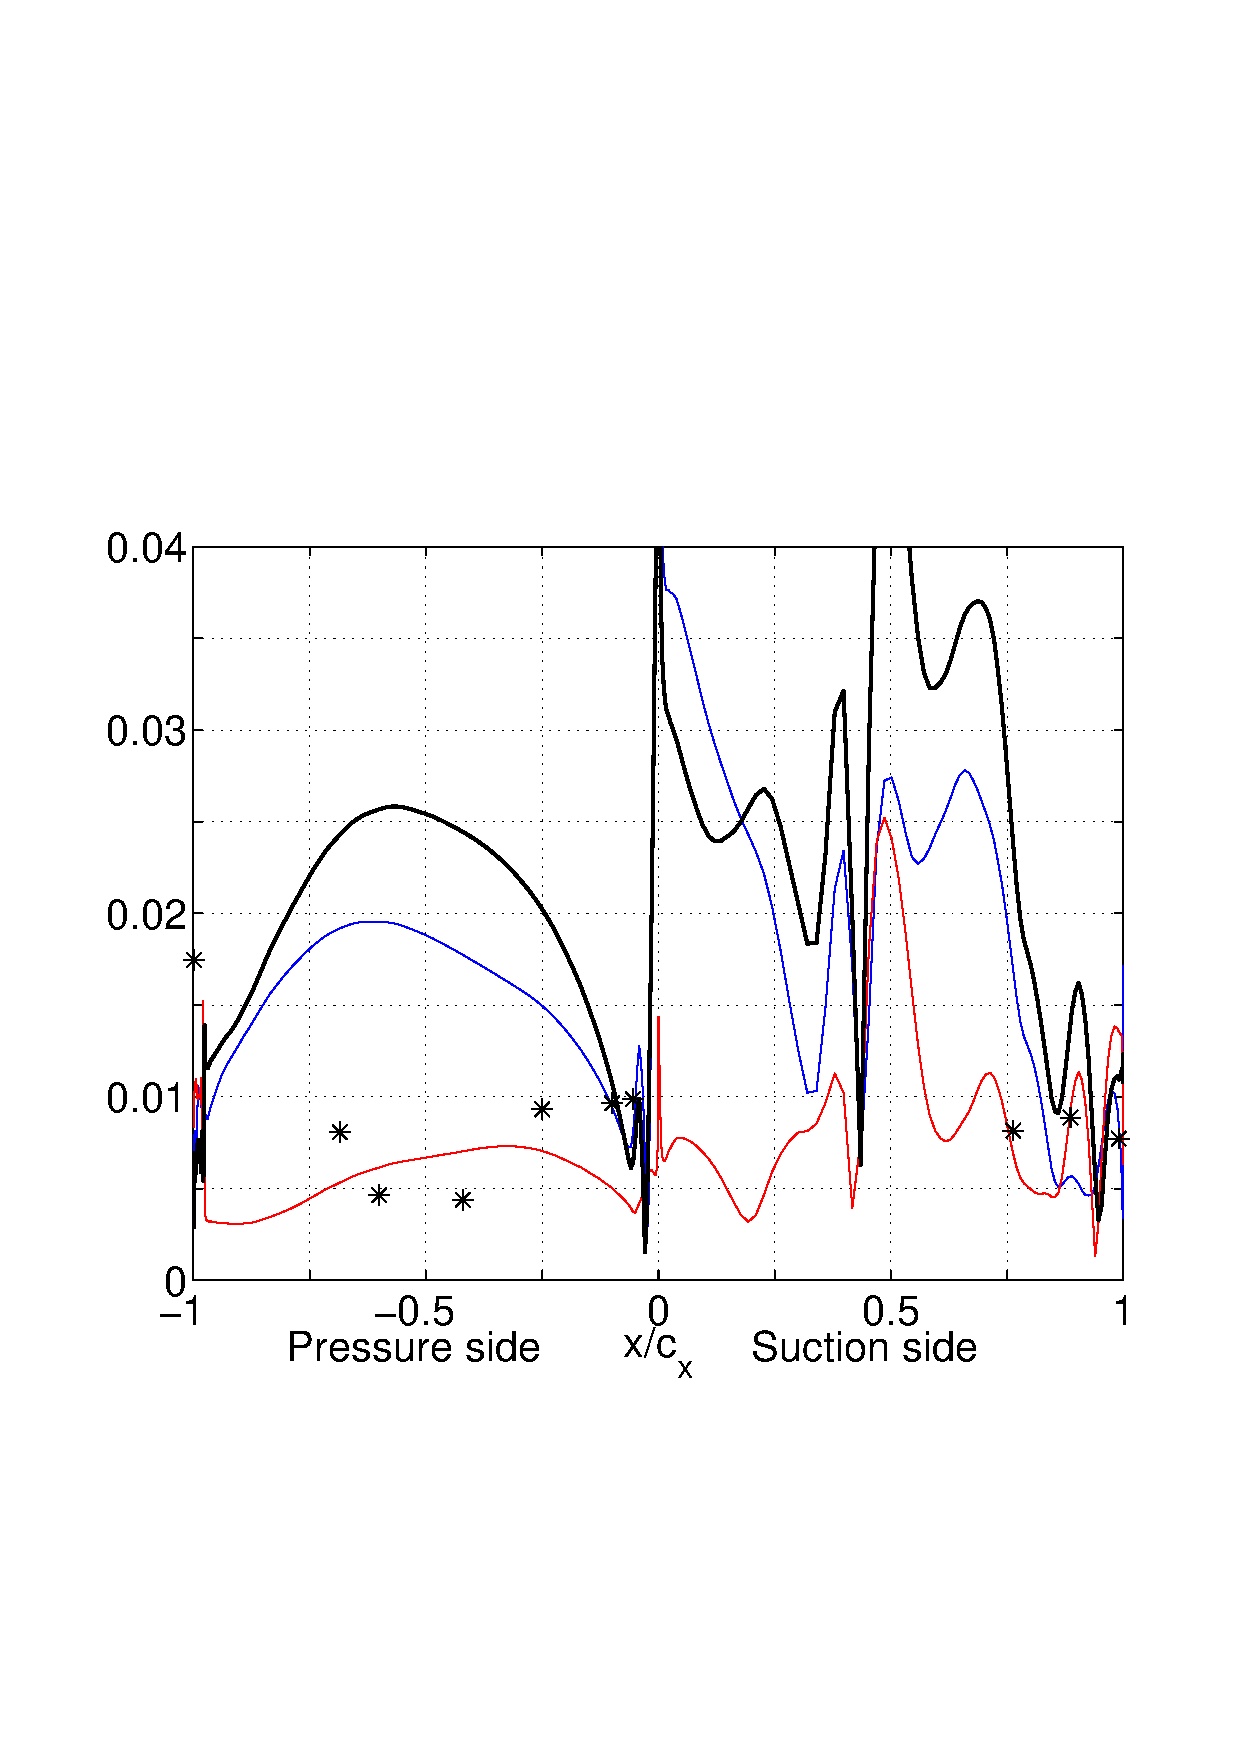
\includegraphics[width=70mm,clip=t]{CHAP_RT27/FIGURE/amps2m1.pdf}
         &
        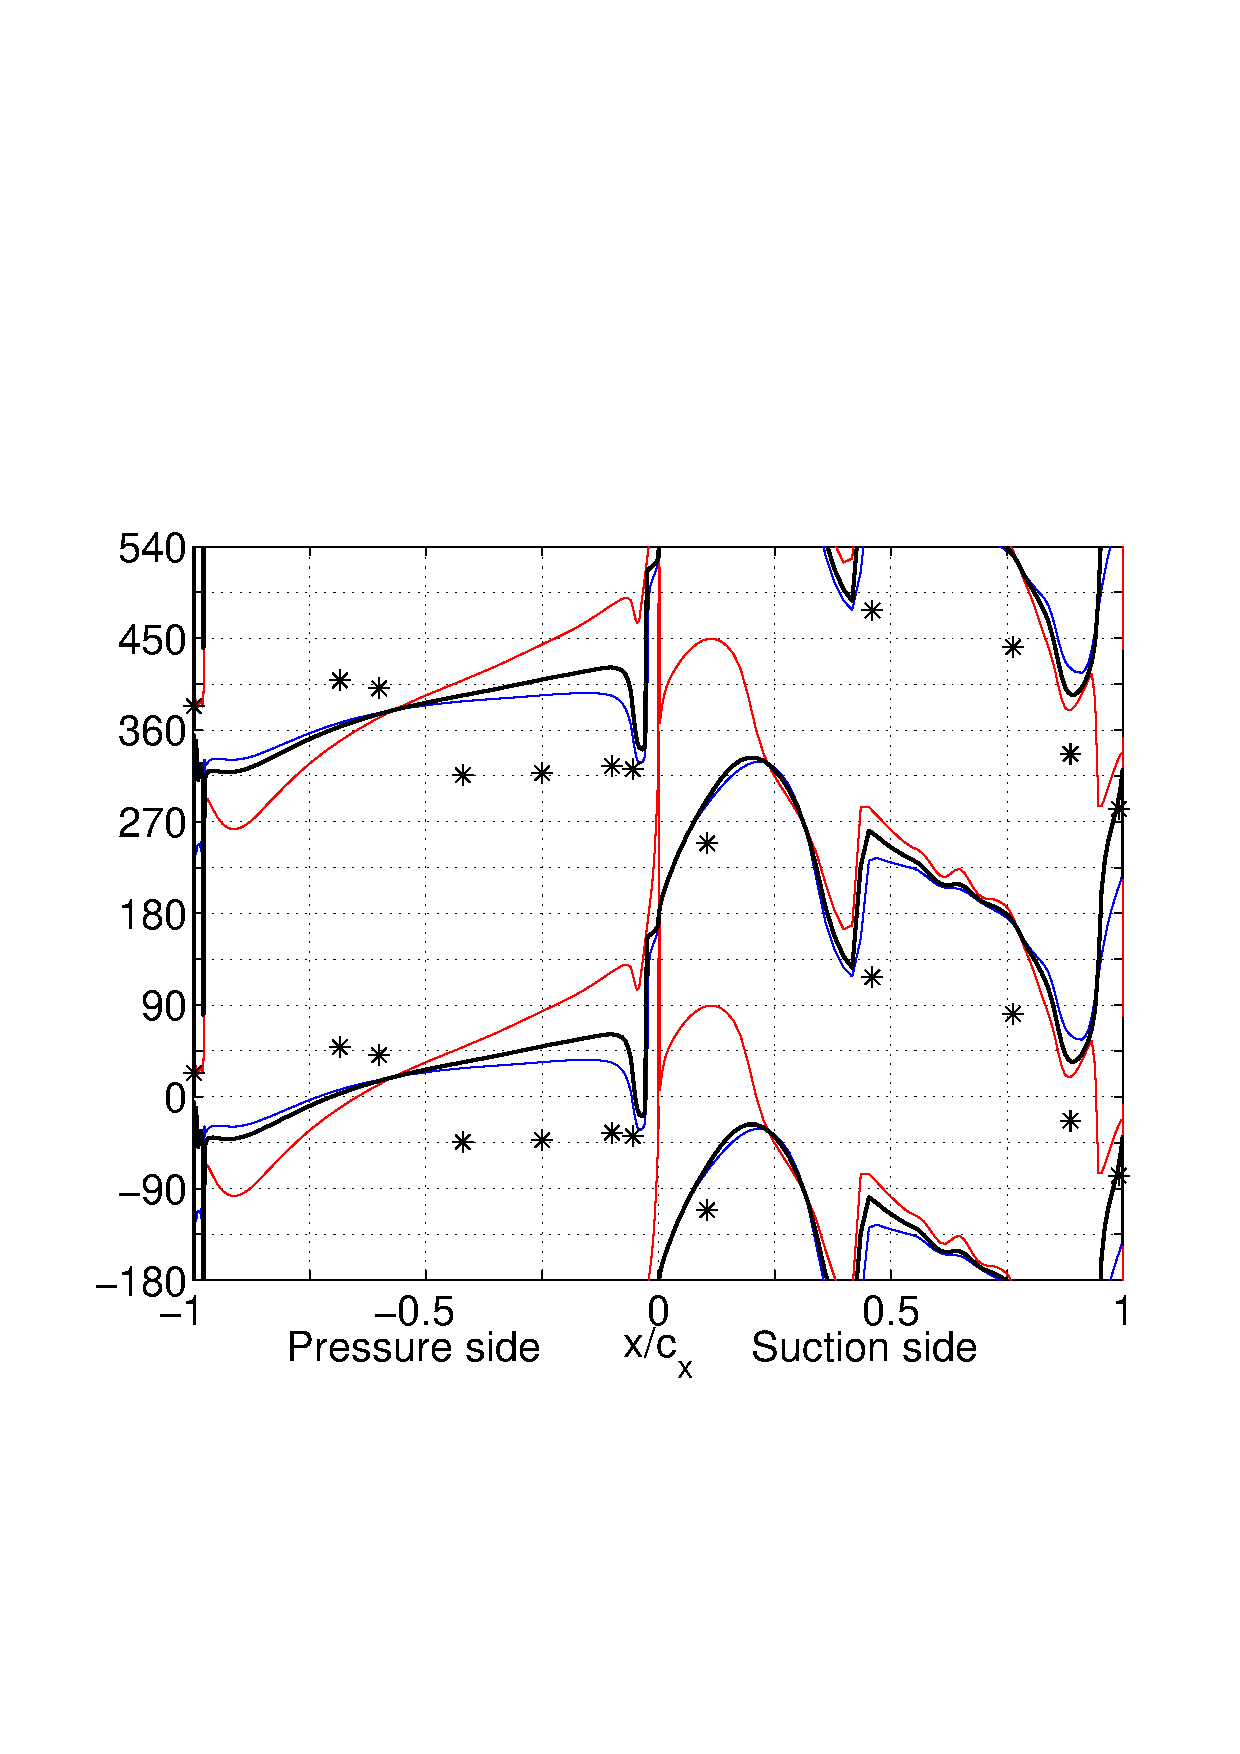
\includegraphics[width=70mm,clip=t]{CHAP_RT27/FIGURE/phas2m1.pdf}
       \end{tabular}}
      \vspace{-5mm}\\
     \subfigure[Mid-height section ($50\%$ span)]
      {\begin{tabular}{ll}
        \hspace{-5mm}
        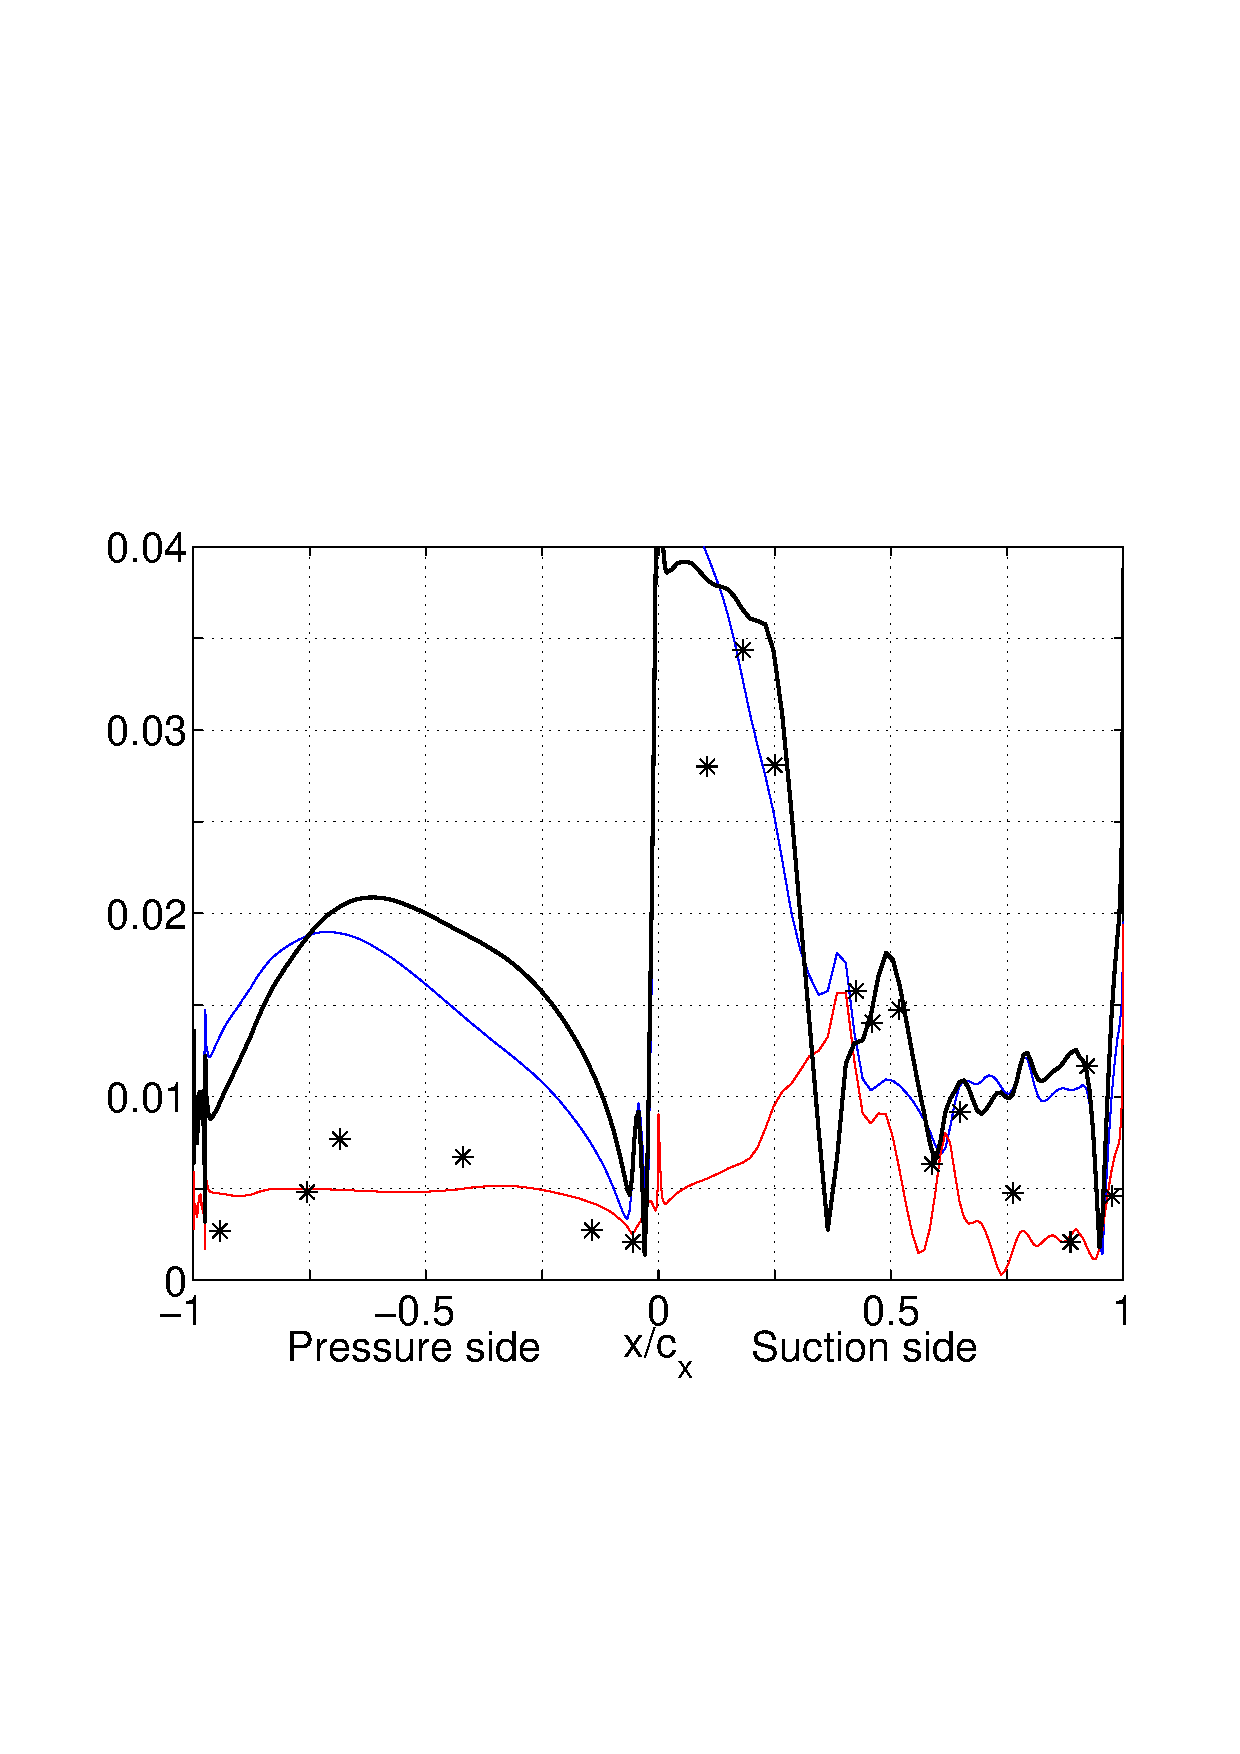
\includegraphics[width=70mm,clip=t]{CHAP_RT27/FIGURE/amps3m1.pdf}
         &
        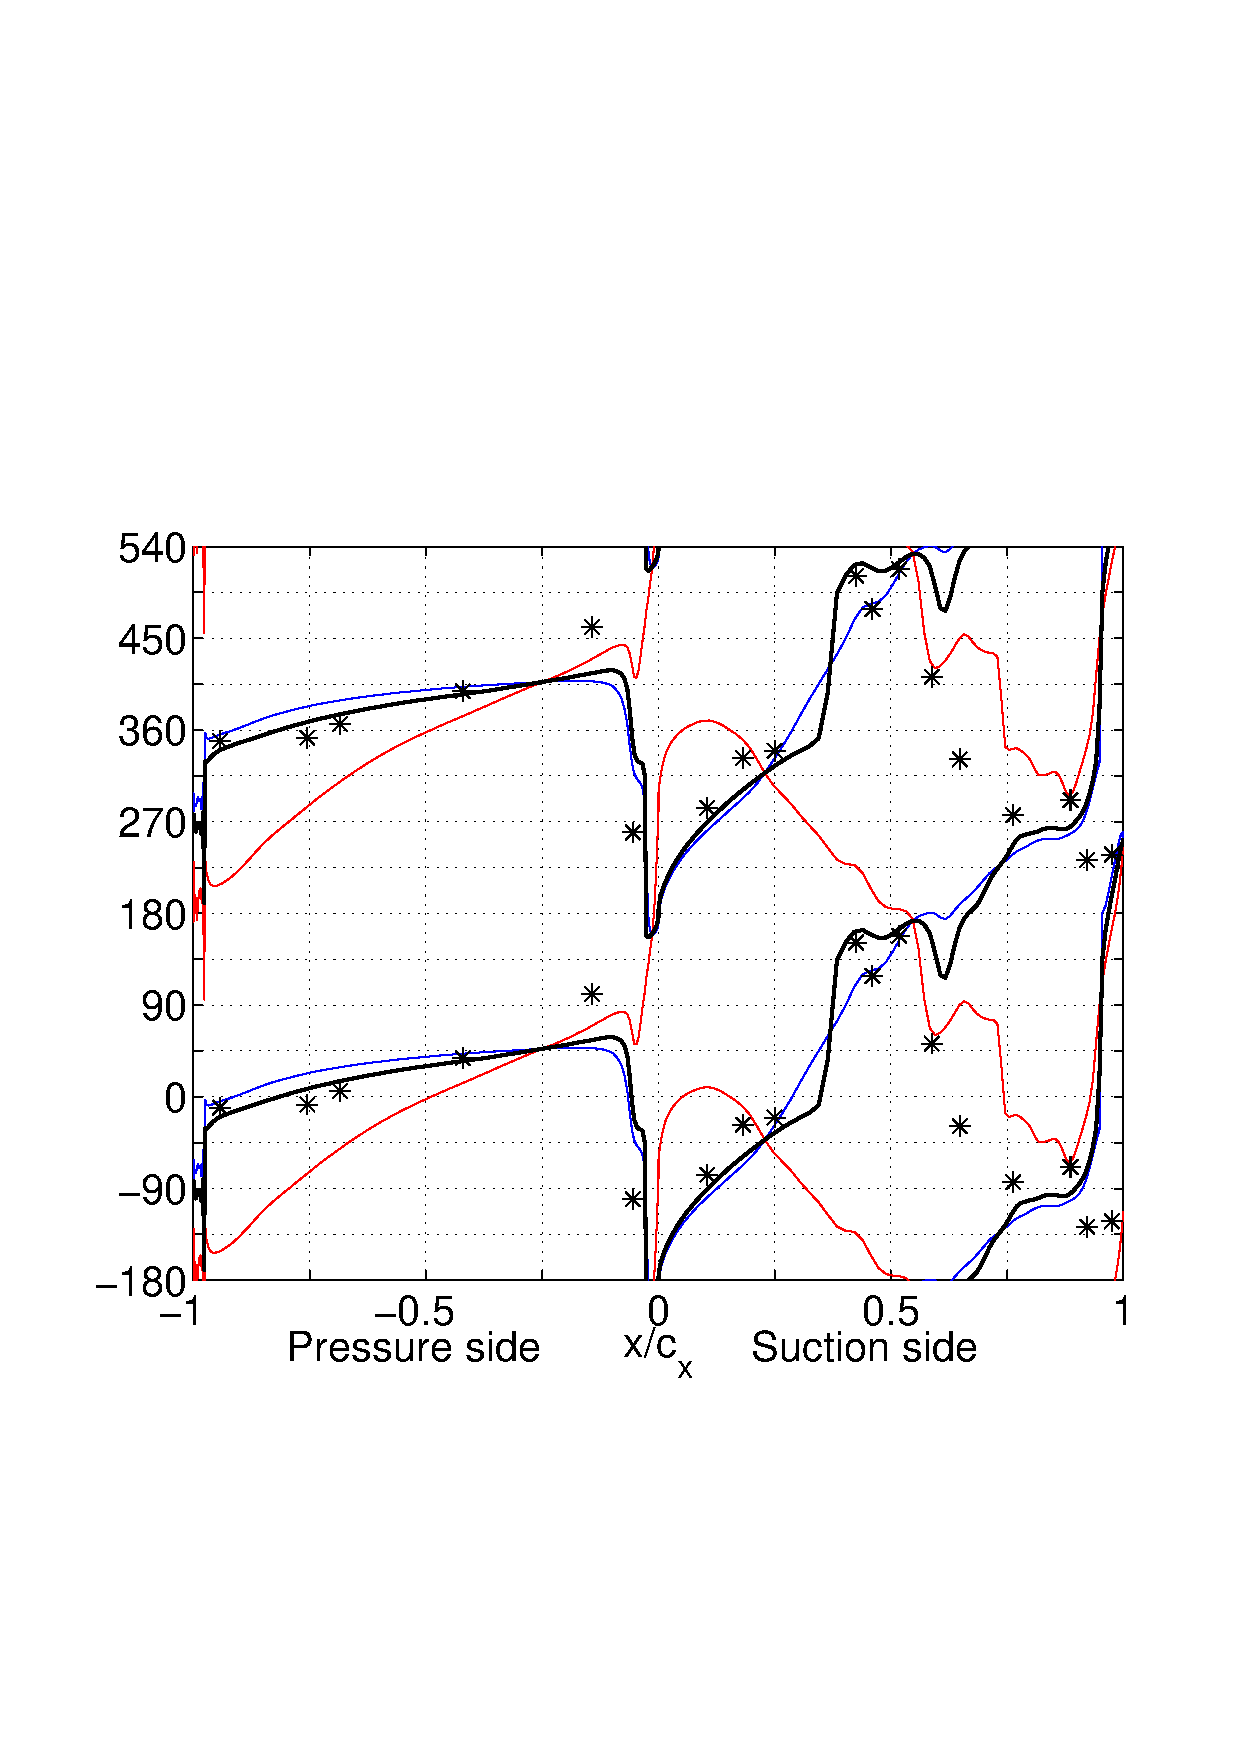
\includegraphics[width=70mm,clip=t]{CHAP_RT27/FIGURE/phas3m1.pdf}
       \end{tabular}}
      \vspace{-5mm}\\
     \subfigure[tip section ($95\%$ span)]
      {\begin{tabular}{ll}
        \hspace{-5mm}
        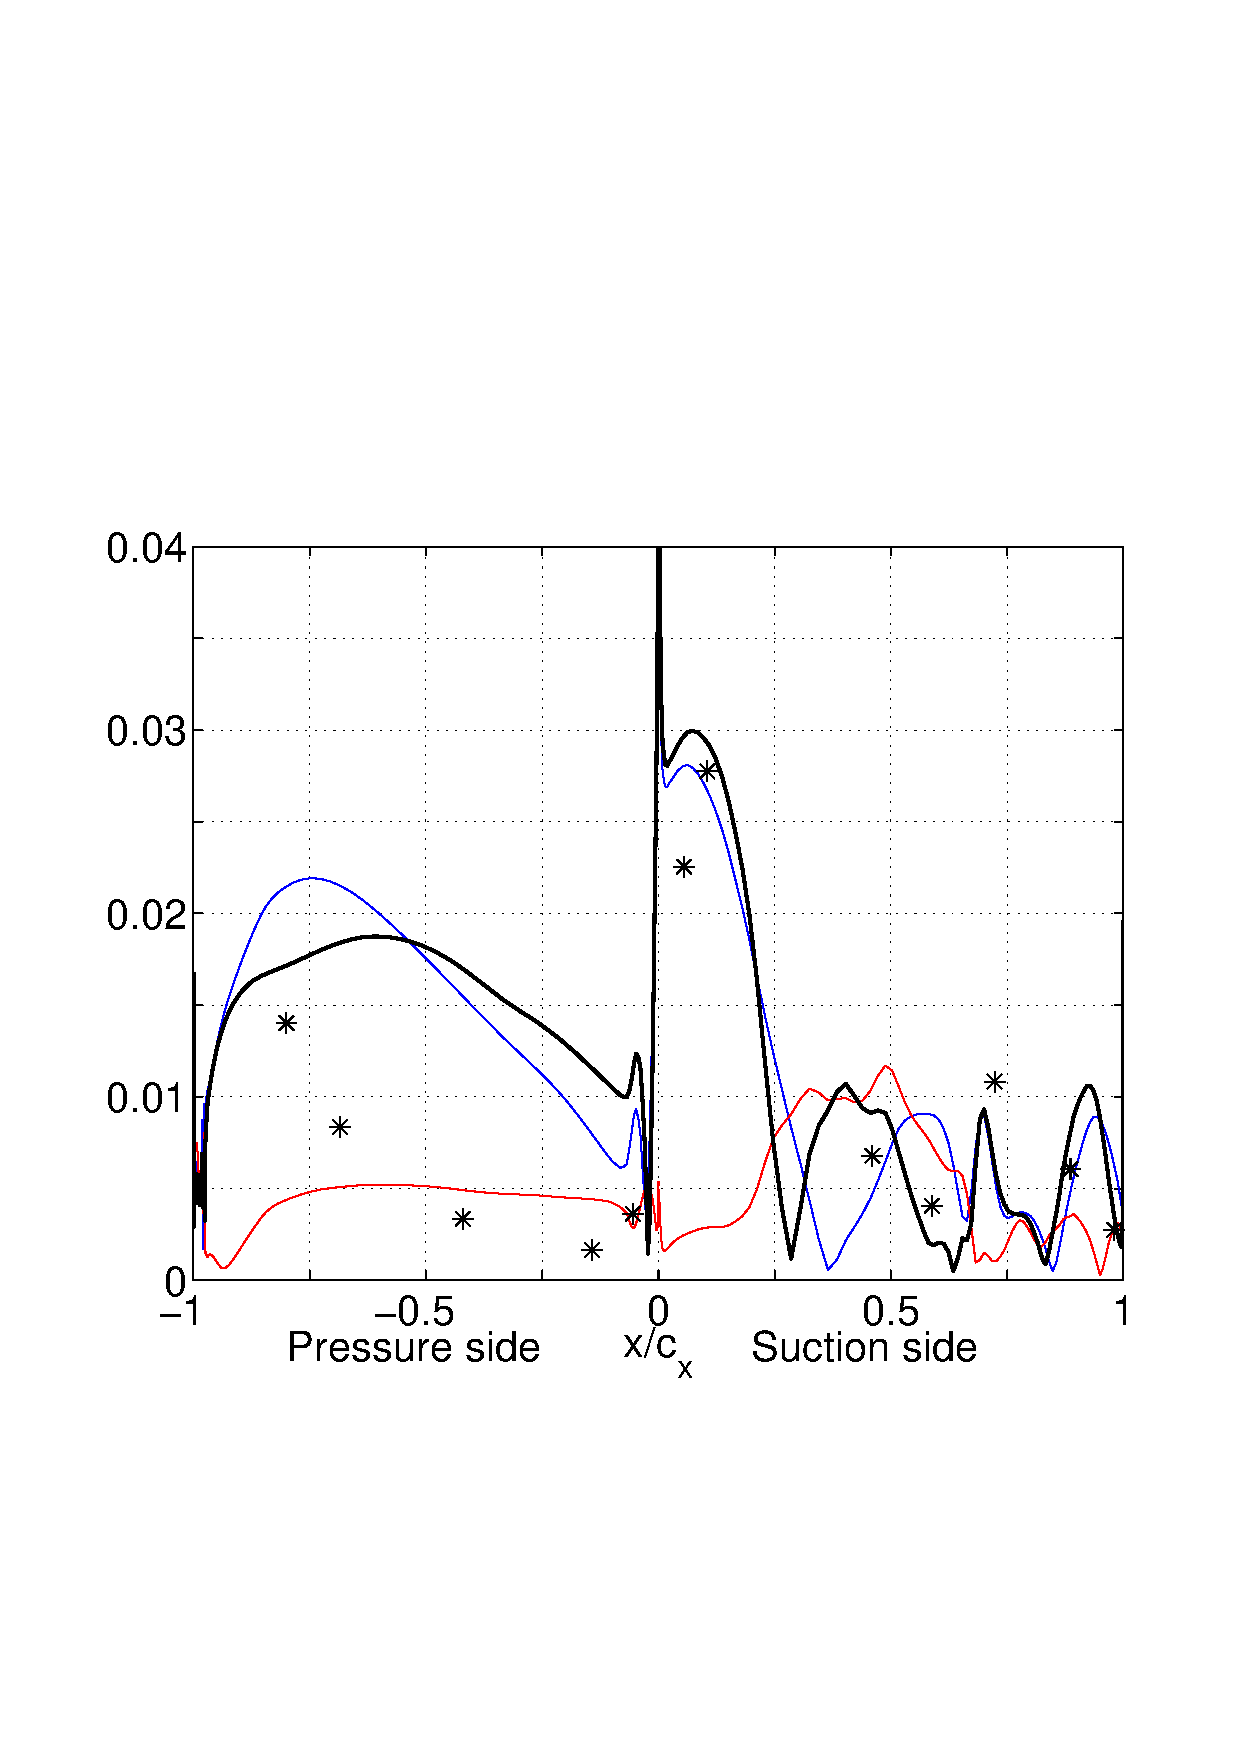
\includegraphics[width=70mm,clip=t]{CHAP_RT27/FIGURE/amps5m1.pdf}
         &
        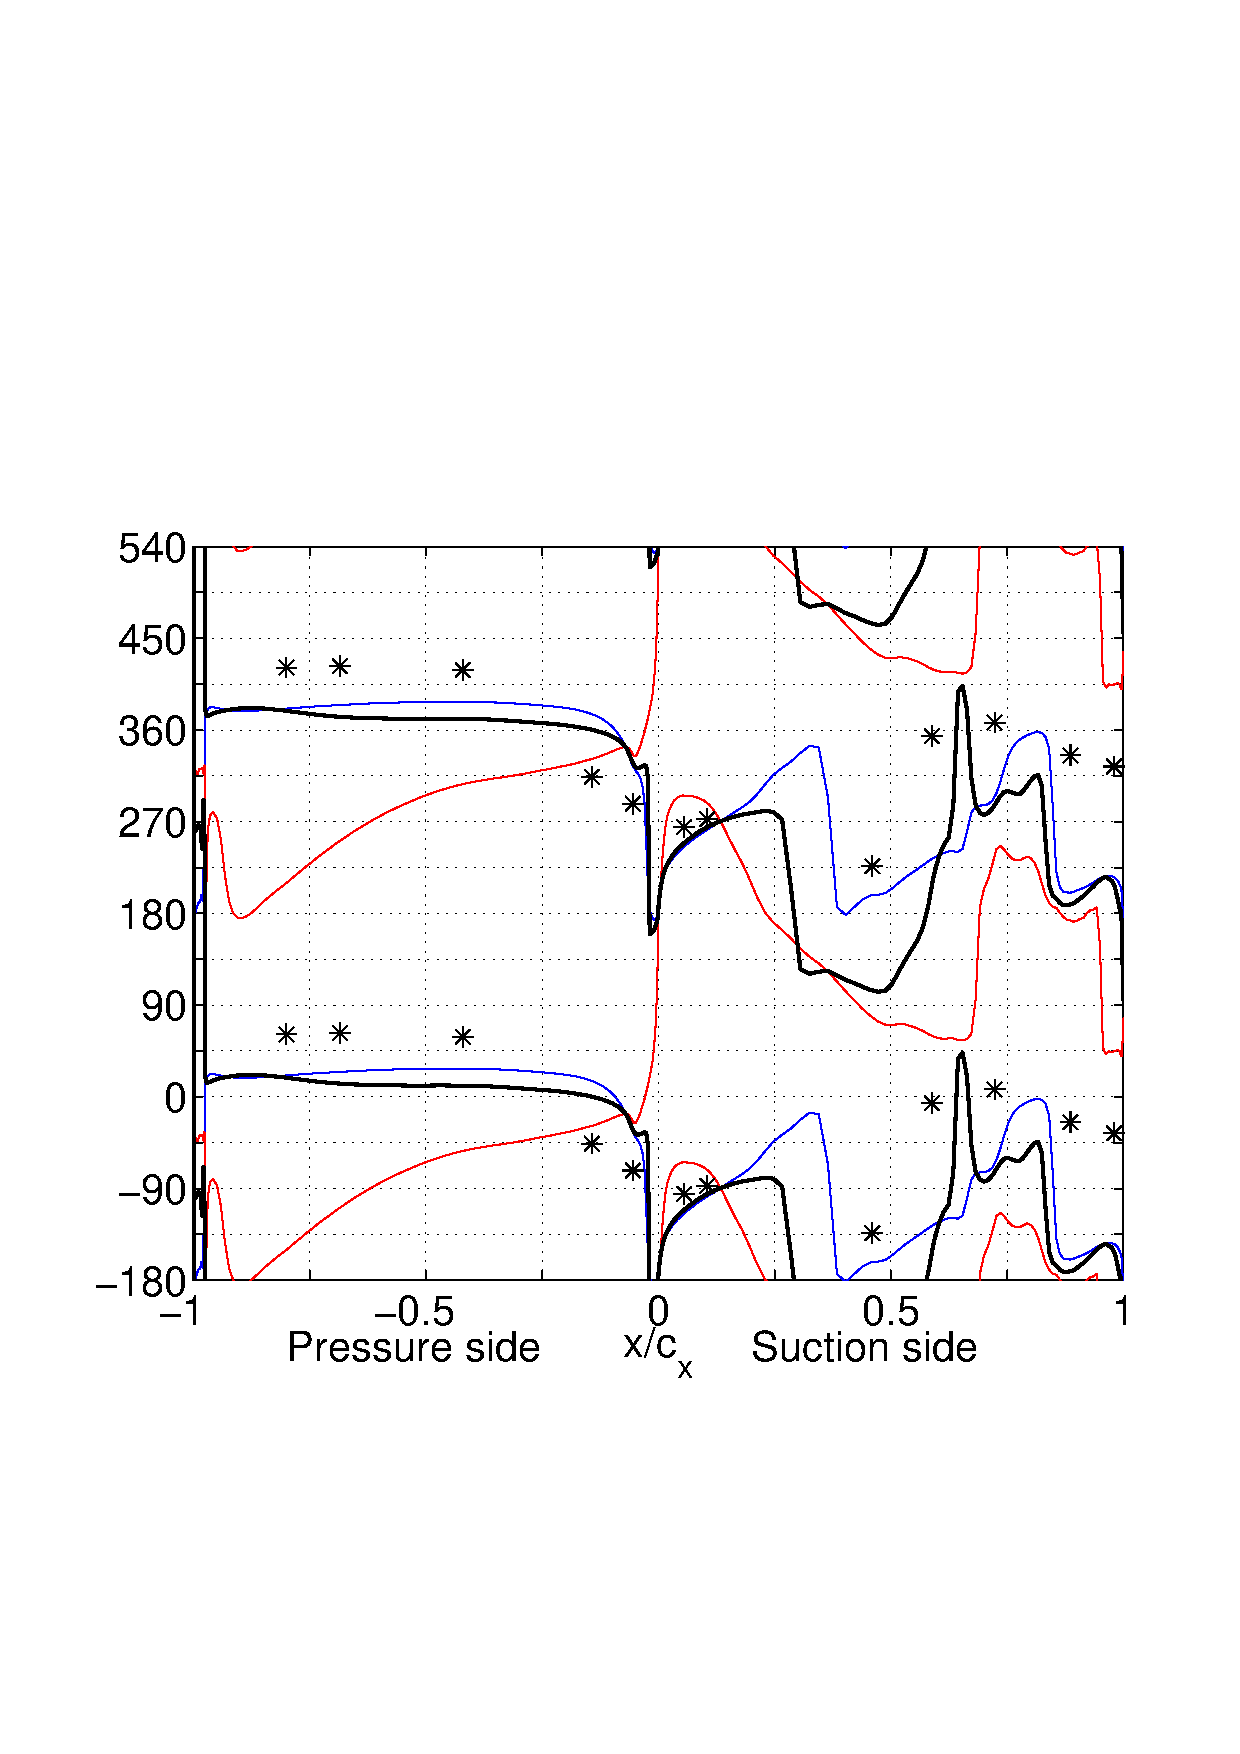
\includegraphics[width=70mm,clip=t]{CHAP_RT27/FIGURE/phas5m1.pdf}
       \end{tabular}}
   \end{tabular}
  \end{flushleft}
  \vspace{-8mm}
  \caption{Amplitude (left) and Phase (right) of
           first Fourier component of unsteady pressure $p/p_0$
           in the RT27a rotor blade.
           Potential mode (blue), vortical mode (red),
           superposed (black) and measured (*).}
  \label{rt27_unsteady3d_1.fig}
\end{figure}
%
%
 Fig. \ref{rt27_unsteady3d_1.fig} shows the amplitude and the
 phase angle of the first Fourier component of the unsteady pressure
 for these three radial sections.
 A striking feature of Fig. \ref{rt27_unsteady3d_1.fig} is that
 the pressure amplitude on the pressure surface is overpredicted
 for all three sections.
 This significant discrepancy is more evident in
 the mid-root section where shape of the predicted amplitude shows a maximum
 at mid-chord whereas the measured data indicate a minimum.
 On the other hand, at mid-height and tip, the shape of the predicted amplitude
 is similar to the measured ones even though there is a factor of two discrepancy.
 As it will be discussed in section \ref{linvnon_rt27.sec}, the reason of
 such discrepancy cannot be attributed to a possible
 non-linear behaviour.
%
%
\begin{figure}
  \begin{flushleft}
   \begin{tabular}{l}
     \subfigure[Mid-root section ($10\%$ span)]
      {\begin{tabular}{ll}
        \hspace{-5mm}
        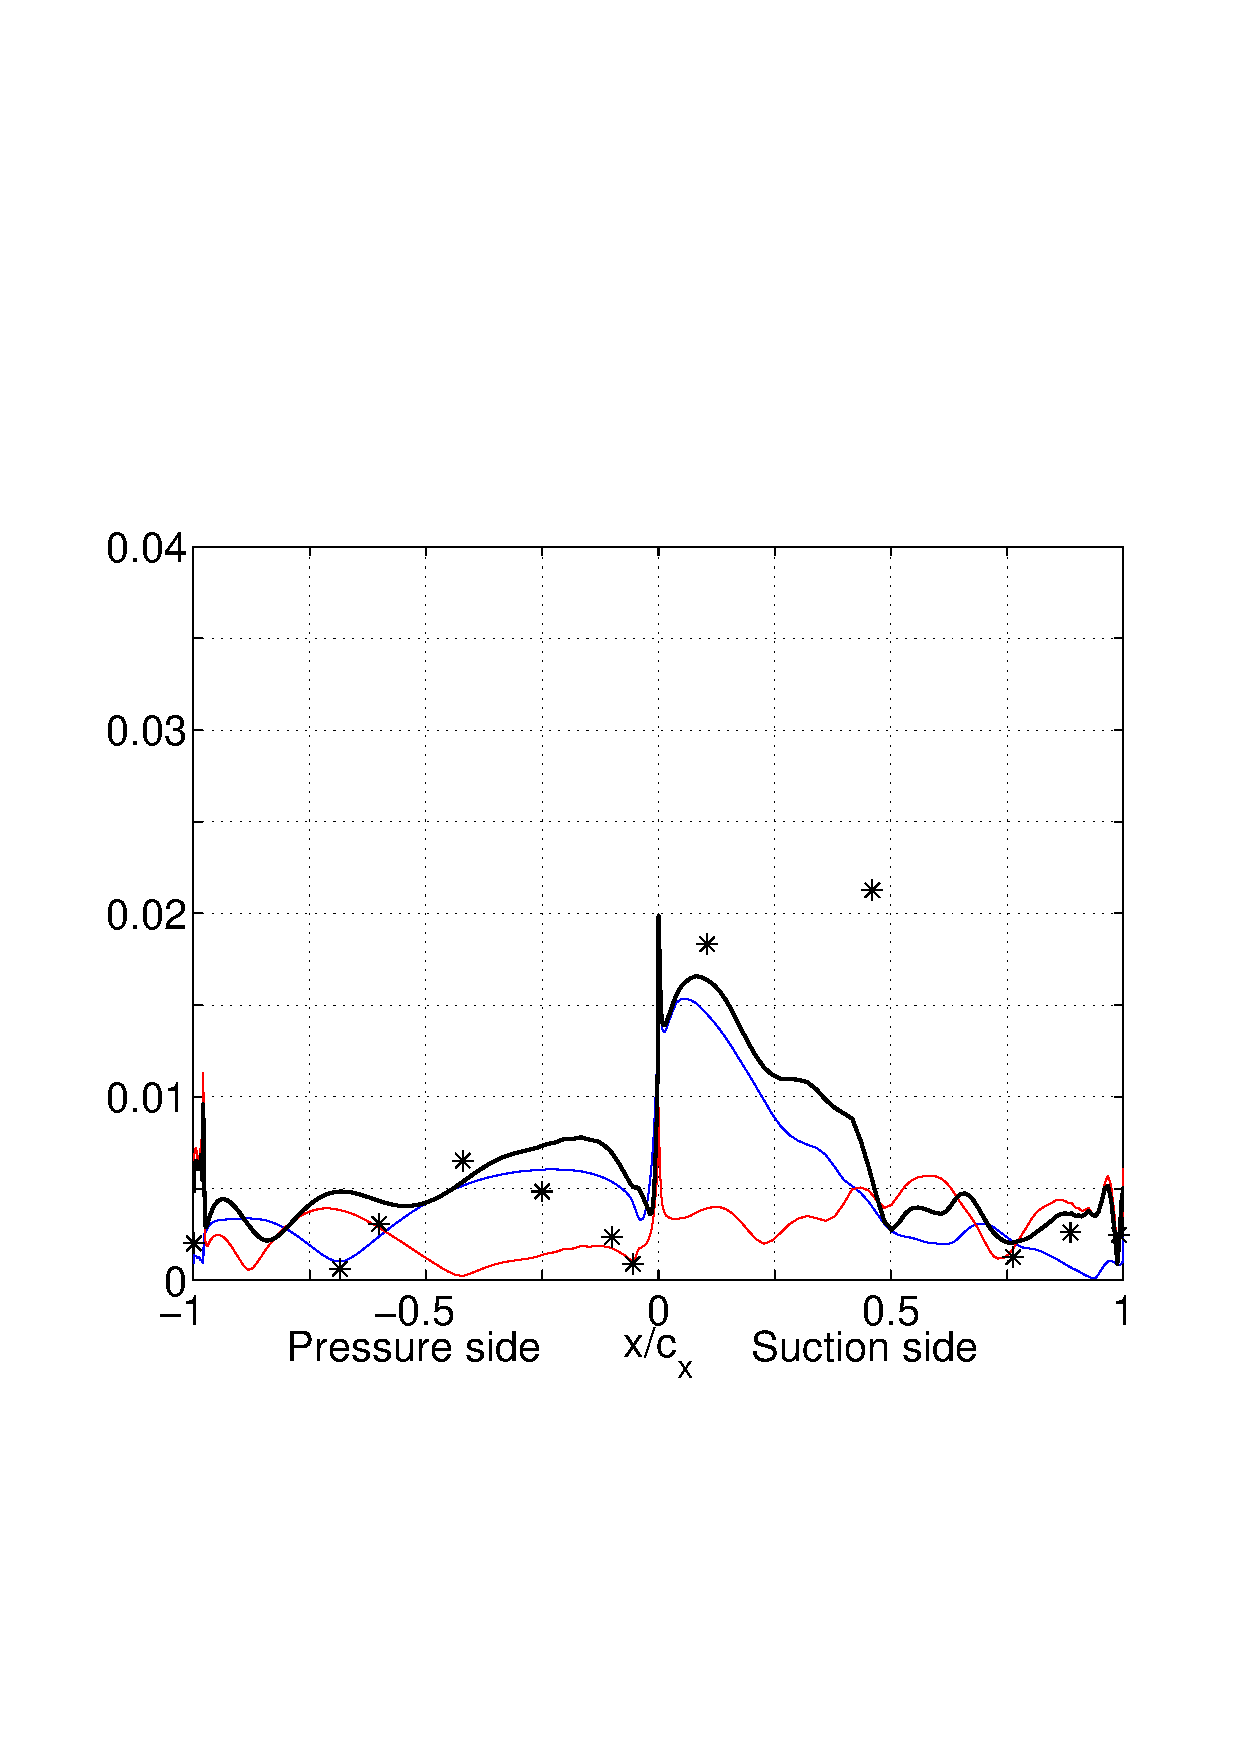
\includegraphics[width=70mm,clip=t]{CHAP_RT27/FIGURE/amps2m2.pdf}
         &
        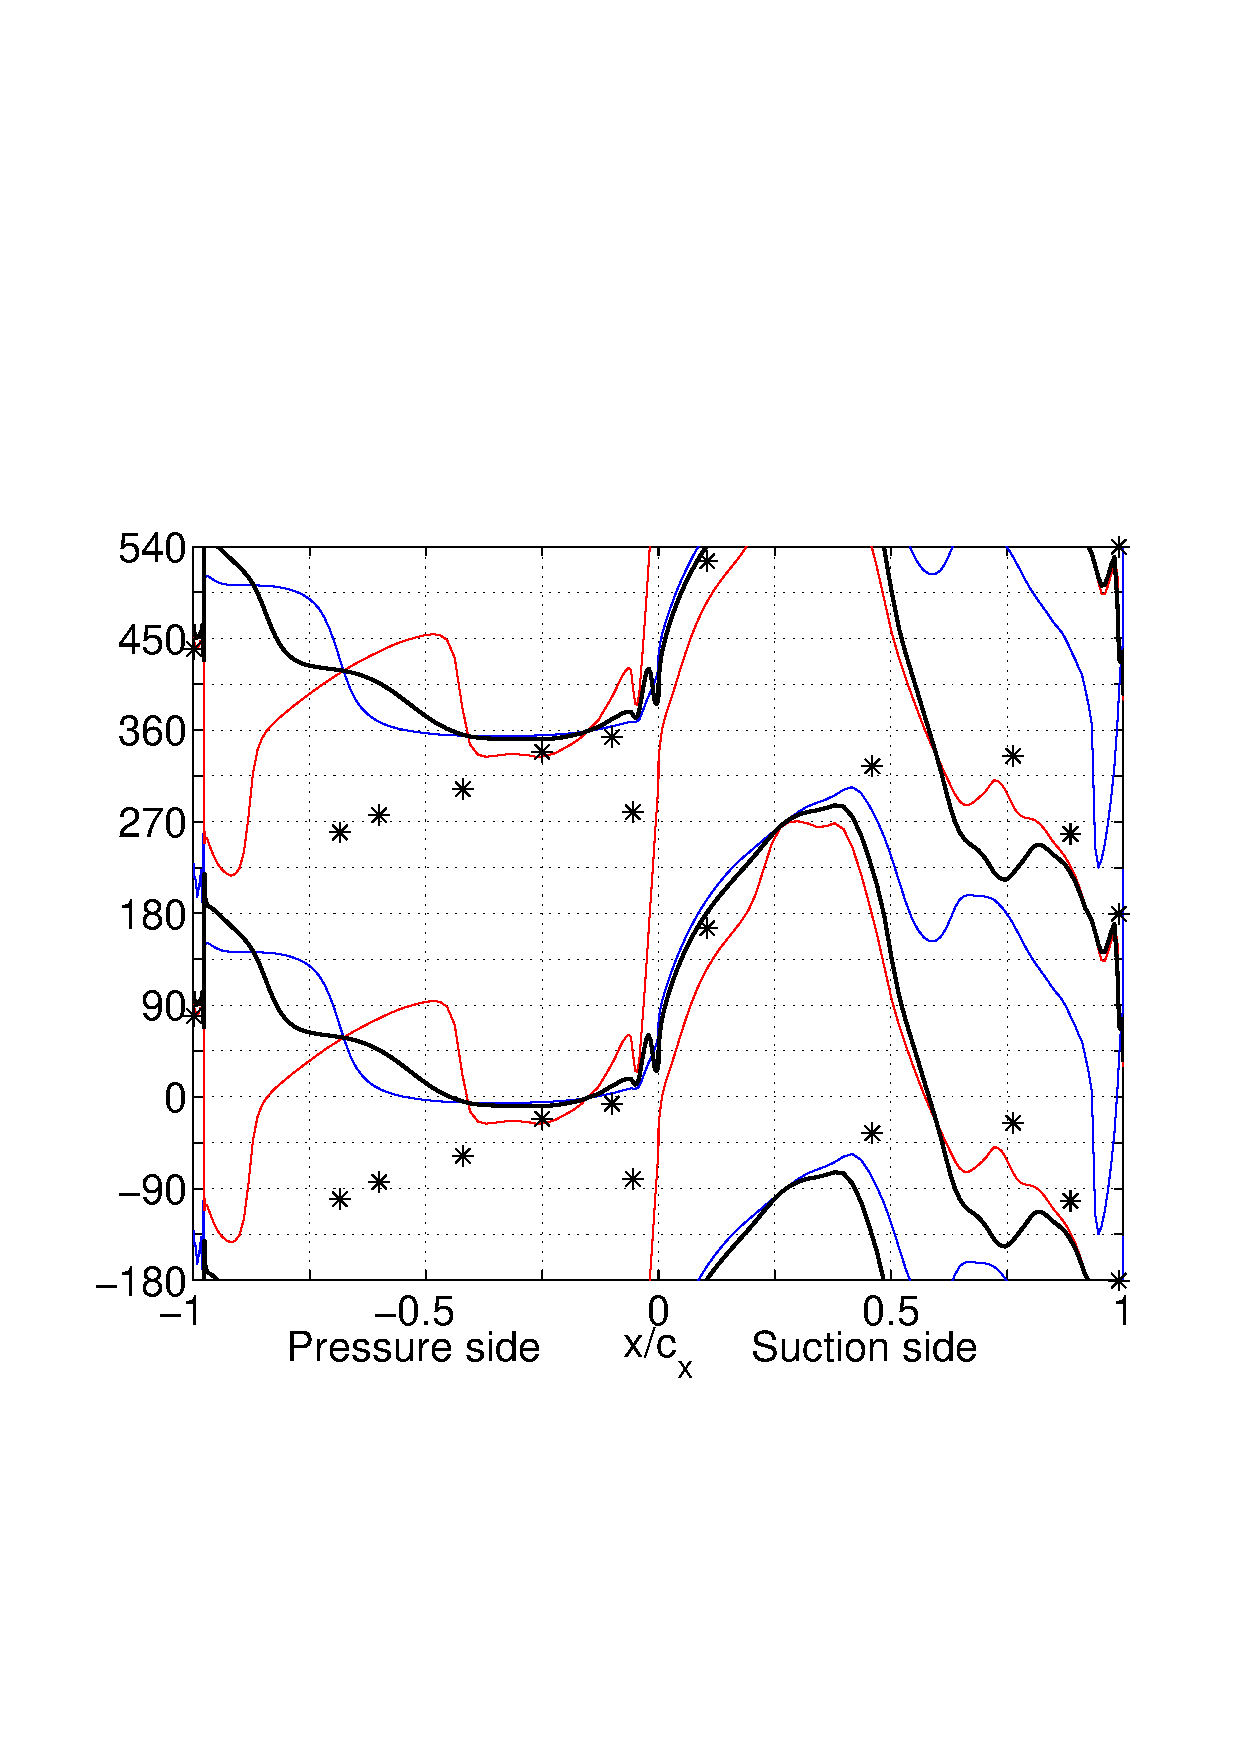
\includegraphics[width=70mm,clip=t]{CHAP_RT27/FIGURE/phas2m2.pdf}
       \end{tabular}}
      \vspace{-5mm}\\
     \subfigure[Mid-height section ($50\%$ span)]
      {\begin{tabular}{ll}
        \hspace{-5mm}
        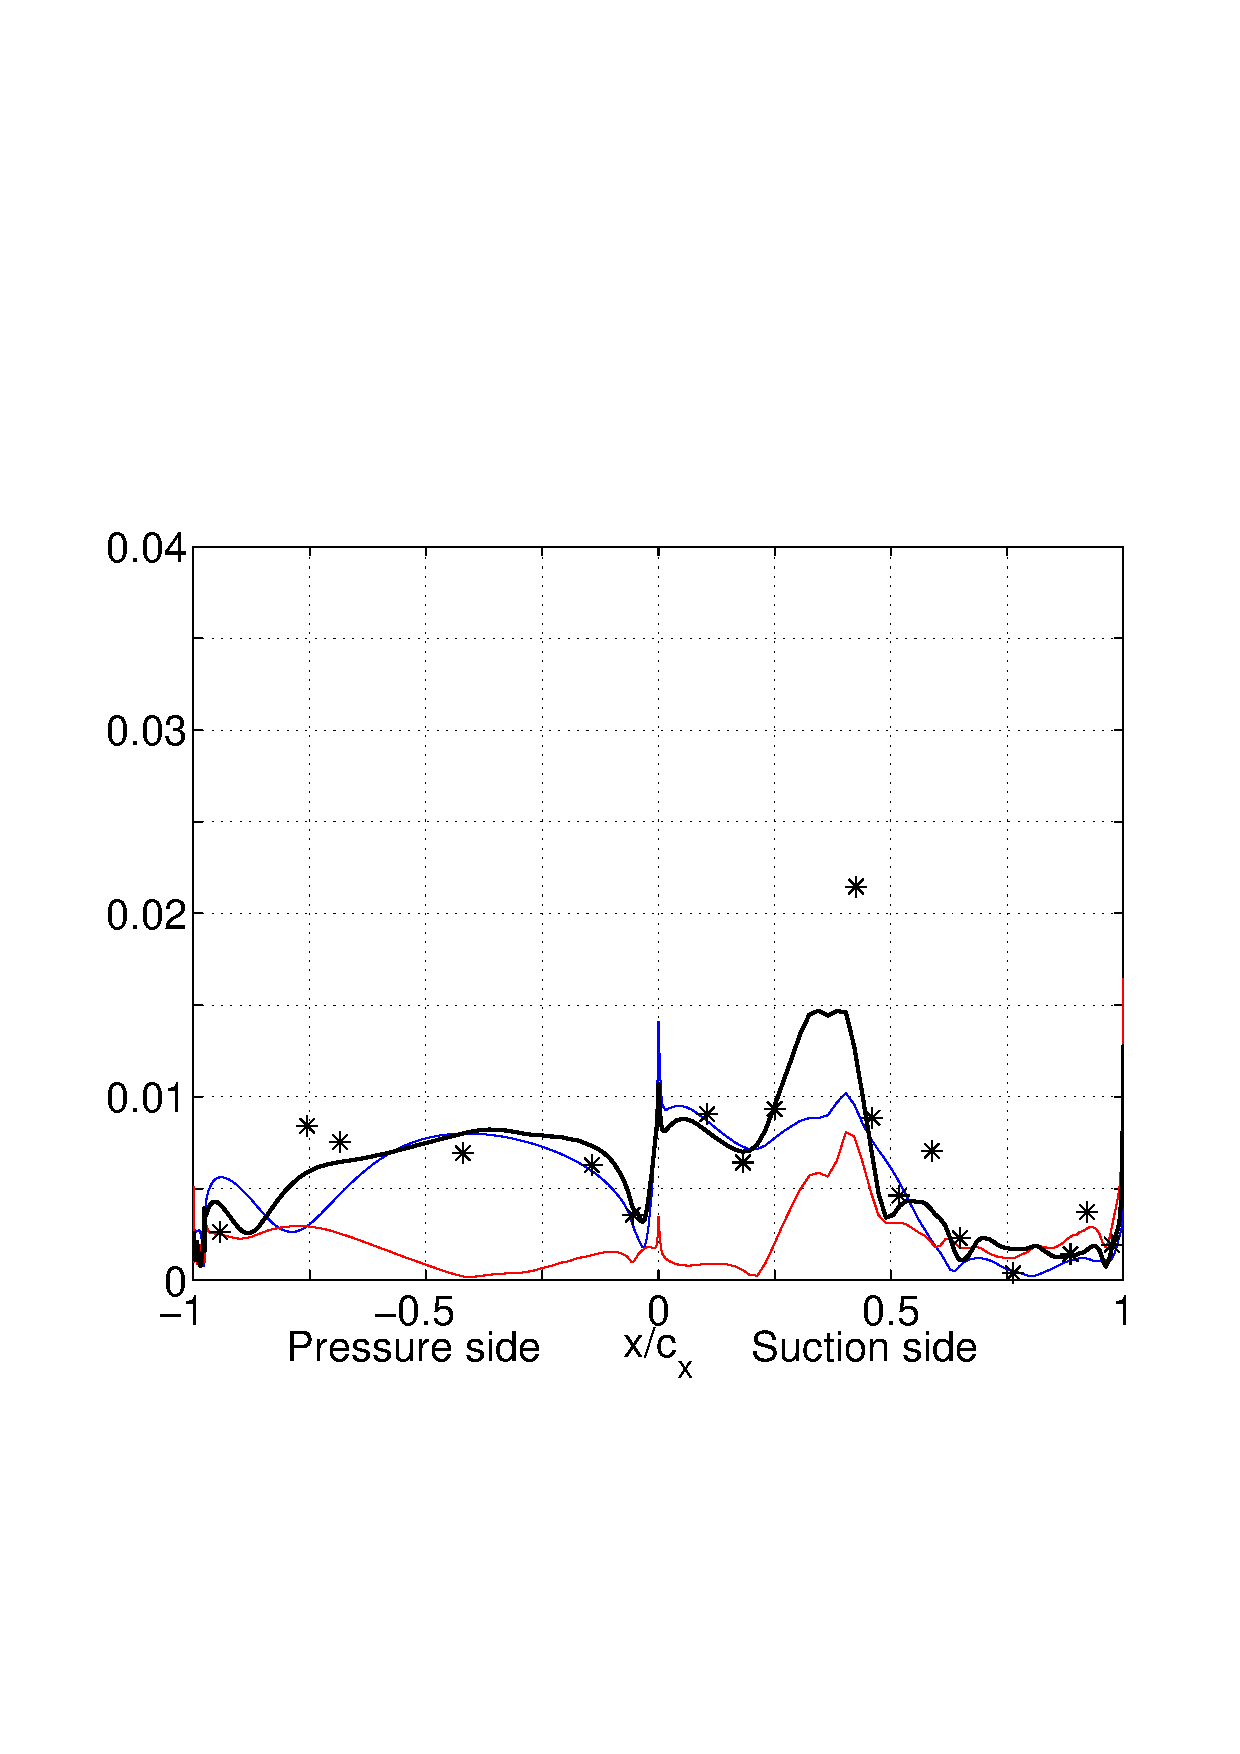
\includegraphics[width=70mm,clip=t]{CHAP_RT27/FIGURE/amps3m2.pdf}
         &
        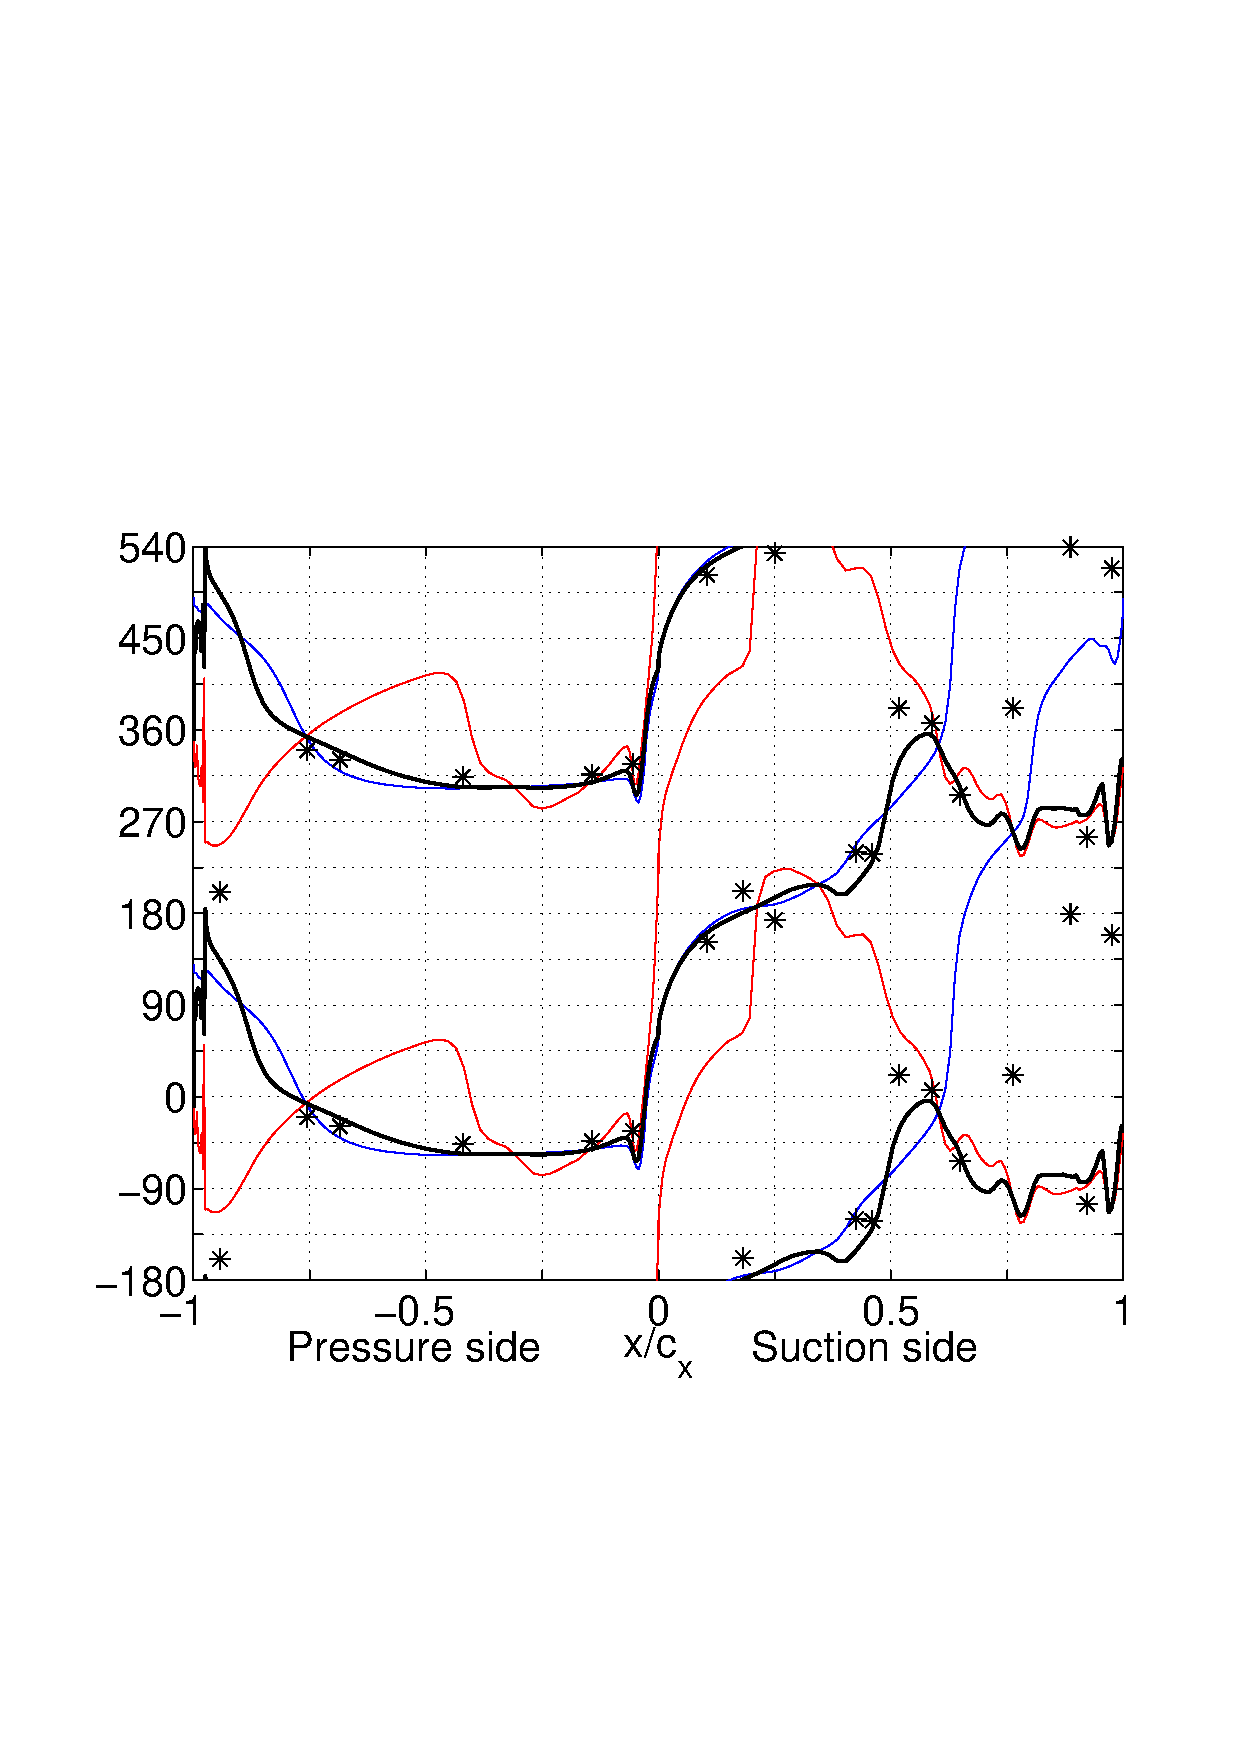
\includegraphics[width=70mm,clip=t]{CHAP_RT27/FIGURE/phas3m2.pdf}
       \end{tabular}}
      \vspace{-5mm}\\
     \subfigure[tip section ($95\%$ span)]
      {\begin{tabular}{ll}
        \hspace{-5mm}
        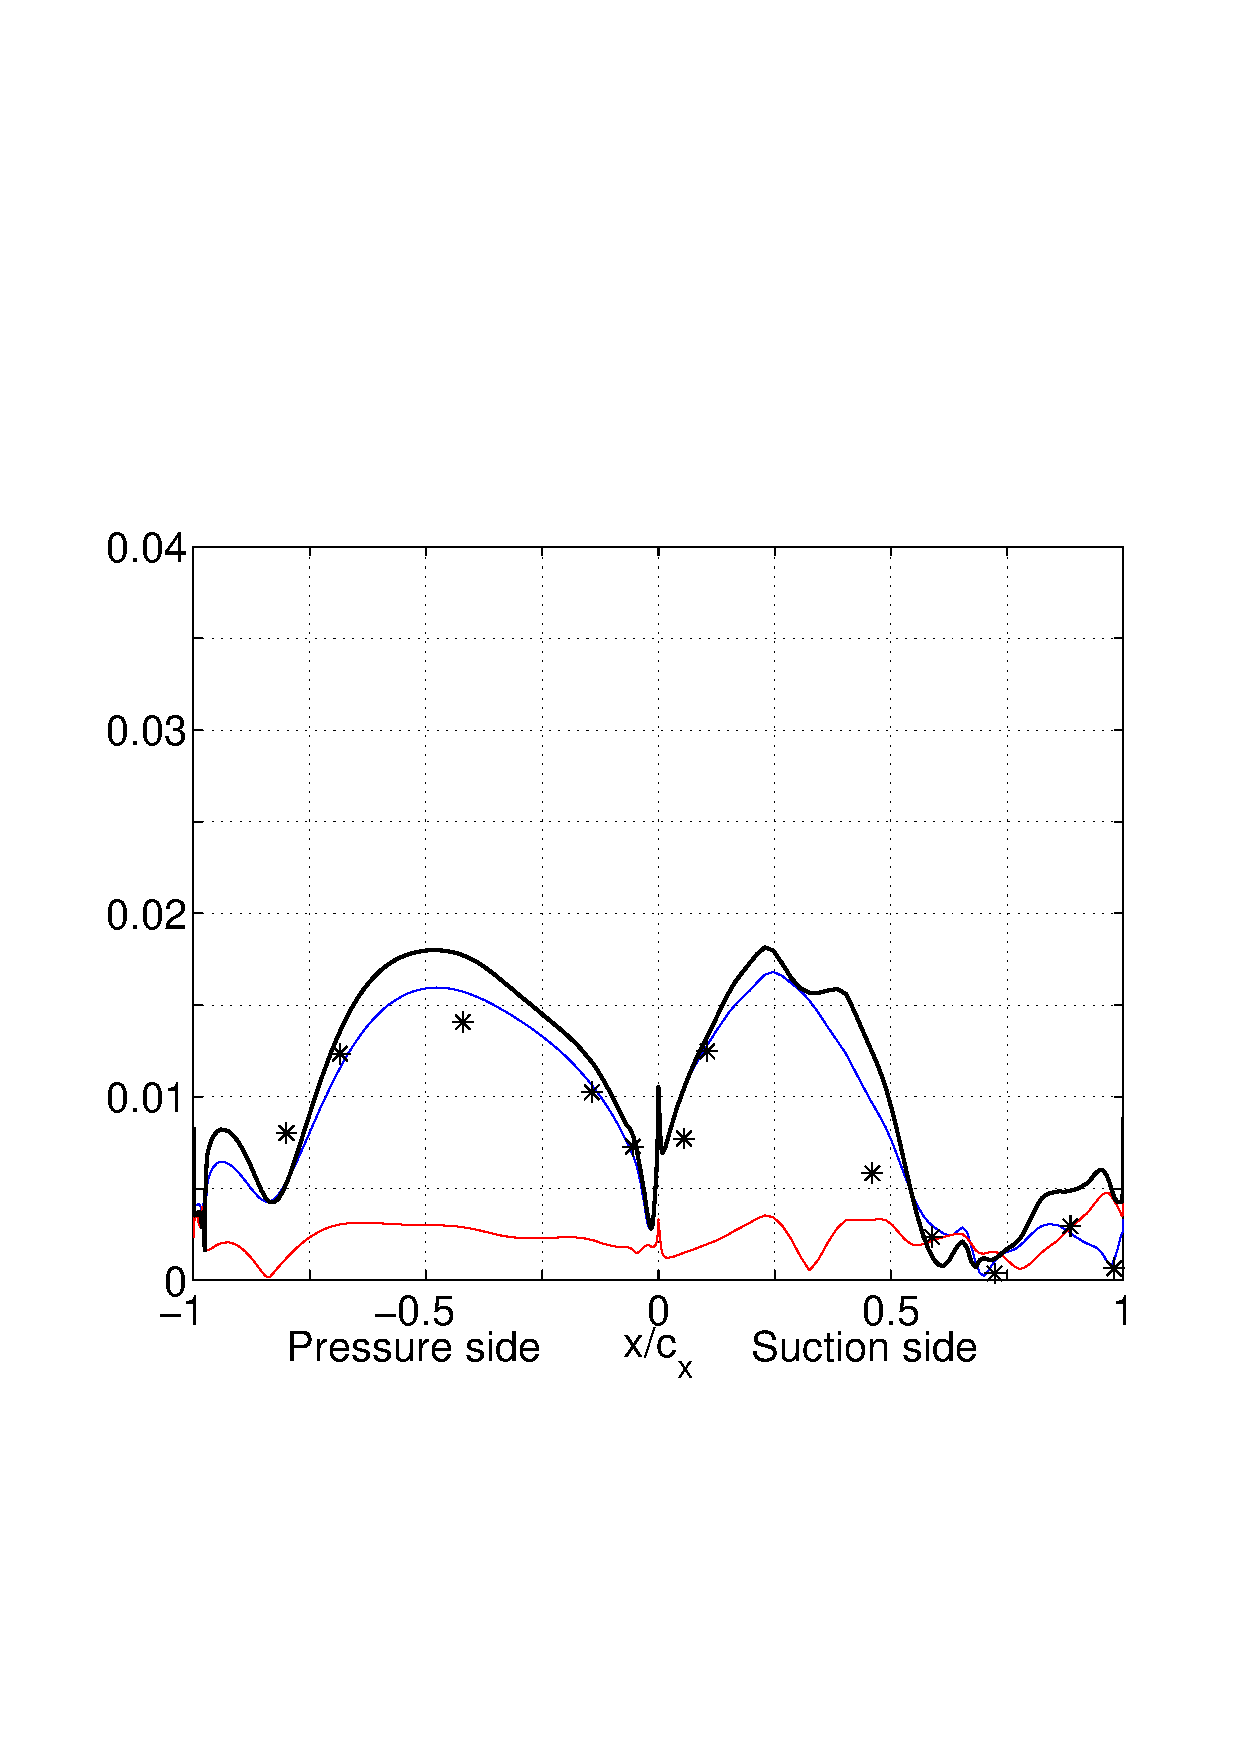
\includegraphics[width=70mm,clip=t]{CHAP_RT27/FIGURE/amps5m2.pdf}
         &
        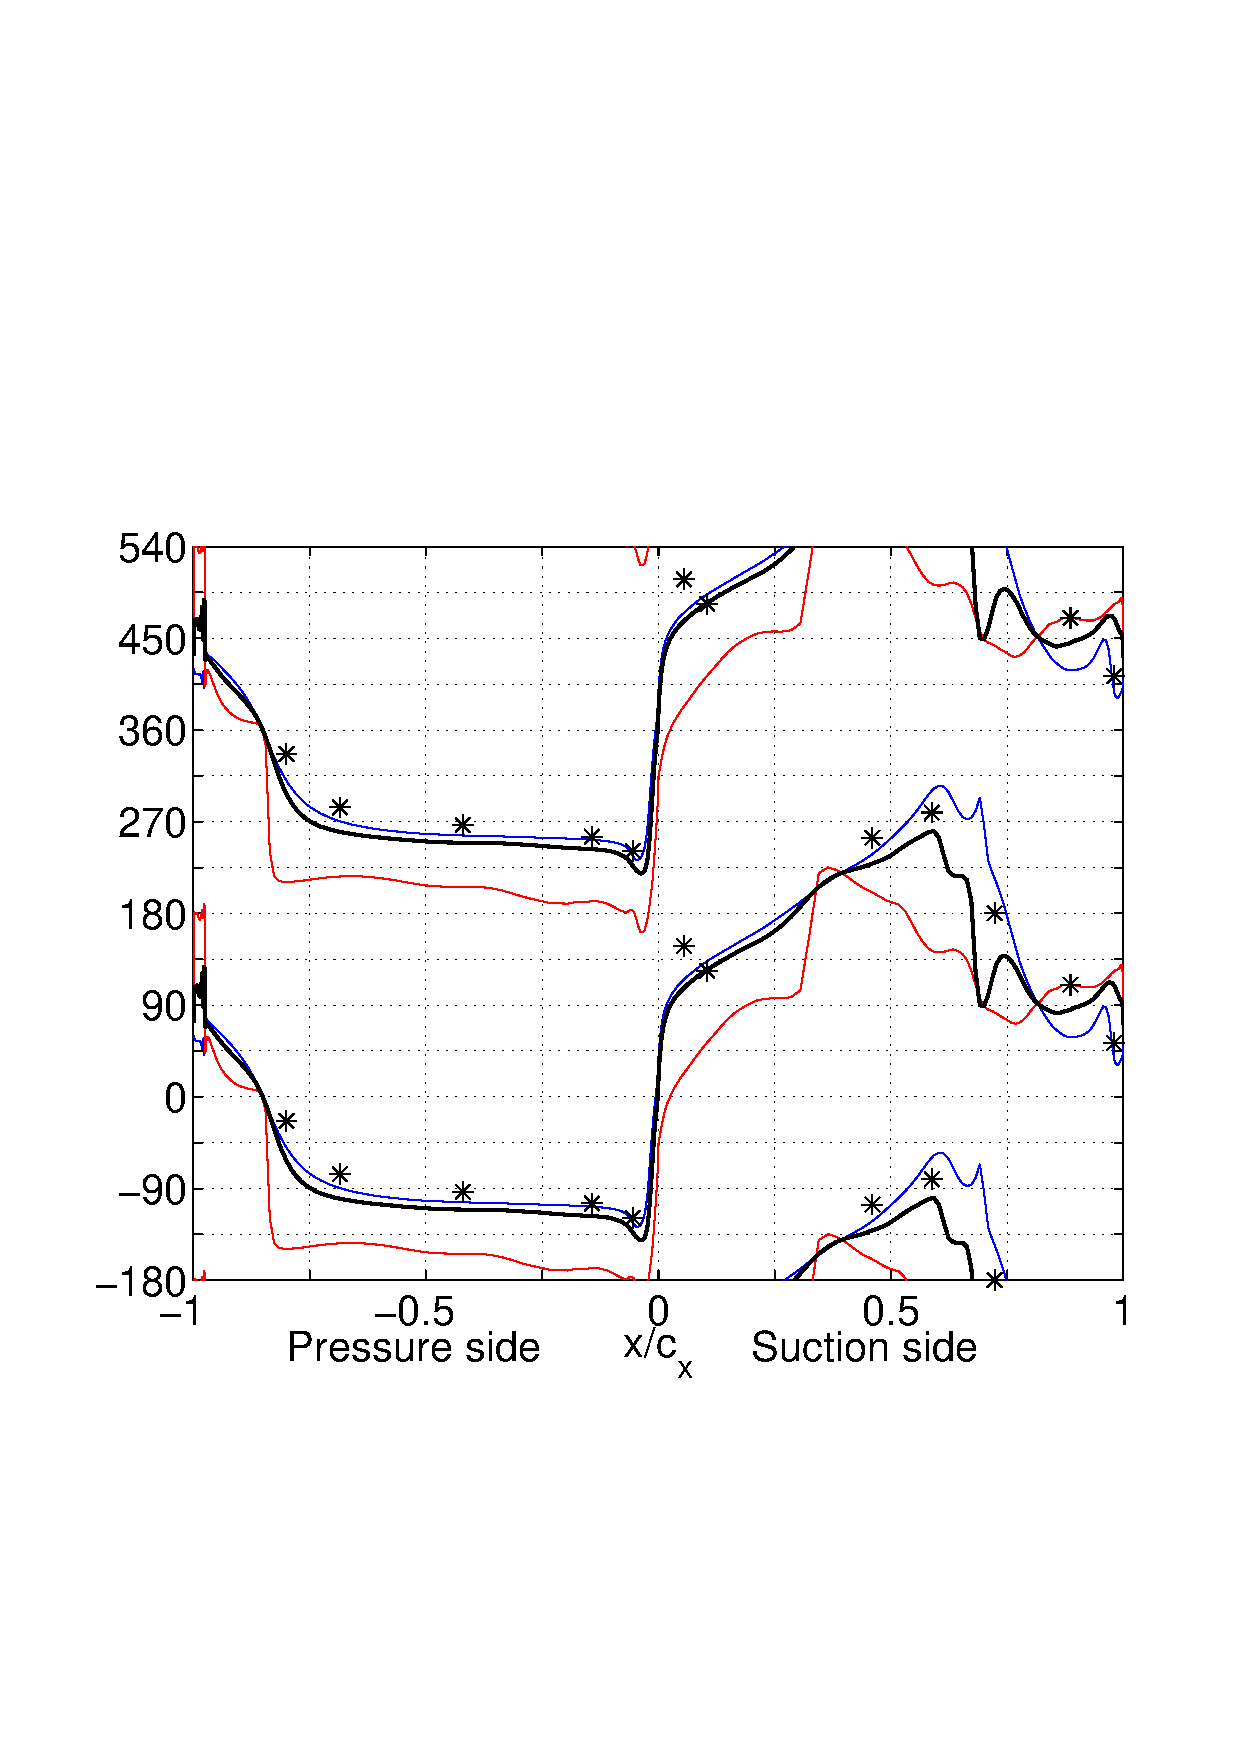
\includegraphics[width=70mm,clip=t]{CHAP_RT27/FIGURE/phas5m2.pdf}
       \end{tabular}}
   \end{tabular}
  \end{flushleft}
  \vspace{-8mm}
  \caption{Amplitude (left) and Phase (right) of
           second Fourier component of unsteady pressure $p/p_0$
           in the RT27a rotor blade.
           Potential mode (blue), vortical mode (red) and
           superposed (black), measured (stars).}
  \label{rt27_unsteady3d_2.fig}
\end{figure}
%
%
 Unlike the amplitude, the phase angle on the pressure side is in
 good agreement especially at mid-height and tip sections.
 The suction side predictions give a good representation,
 both in term of amplitude and phase angle. At mid-height, the suction side
 prediction has some discrepancies with the measured data in the region
 around $x/c\sm{x}\approx 0.75$ where the measured and computed data are out of
 phase and of different amplitudes.

~\newline
 Fig. \ref{rt27_unsteady3d_2.fig} shows the comparison between
 the predicted and measured data for the second Fourier component of the
 unsteady pressure.
 Unlikely the first Fourier component, and perhaps very surprisingly,
 the overall agreement is very good for the all three sections
 both in terms of amplitude and phase angle.
%
%
%
%
%
\subsection{Vortical-flow interaction effects}
\label{rt27_vortical.subsec}
%
 As discussed earlier the vortical flow non-uniformities
 at the NGV outlet are associated with a rotational
 velocity perturbation with zero divergence.
 Such a vortical flow component at the NGV outlet is shown in
 Fig. \ref{ngv_outlet_decomposed1.fig}a for the first two
 tangential Fourier modes.
 Vortical-flow interaction, also labelled wake-rotor interaction,
 has been studied and interpreted by several authors
 (Hodson \citeyearNP{Hodson:1}, Giles \citeyearNP{Giles:2},
 Korakianitis \citeyearNP{Kora:1}, \citeyearNP{Kora:2},
 \citeyearNP{Kora:3}) and it is now fairly well understood.
 Before analysing the hub-to-tip distribution
 of the pressure amplitude, a brief description of the wake-rotor
 interaction at mid-height section is given.

~\newline
 Figs. \ref{rt27_vortical2d_1.fig} and \ref{rt27_vortical2d_2.fig}
 show the dimensionless absolute velocity and pressure fluctuations
 together with the unsteady particle traces during one blade passing
 cycle in the rotor passage.
 The wakes are first bent by the potential flow field of the rotor
 as shown in Fig. \ref{rt27_vortical2d_1.fig}a.
 When the leading-edge in the rotor stagnation region interacts with
 the lower momentum fluid in the wake, unsteady, recirculating flow
 patterns are established as shown in Fig. \ref{rt27_vortical2d_1.fig}a.
%
\begin{figure}
  \begin{center}
   \begin{tabular}{c}
     \subfigure[t = 0]
       {\hspace{-5mm}
        \includegraphics[width=130mm,clip=t]{CHAP_RT27/FIGURE/unsmidsec_4.pdf}}
       \\
     \subfigure[t = 1/6]
       {\hspace{-5mm}
        \includegraphics[width=130mm,clip=t]{CHAP_RT27/FIGURE/unsmidsec_5.pdf}}
       \\
     \subfigure[t = 2/6]
       {\hspace{-5mm}
        \includegraphics[width=130mm,clip=t]{CHAP_RT27/FIGURE/unsmidsec_6.pdf}}
   \end{tabular}
  \end{center}
  \vspace{-8mm}
  \caption{Vortical-flow interaction in the RT27a rotor passage at
           mid-height section (first Fourier component).
           Unsteady dimensionless absolute velocity fluctuations (left) and
           unsteady particle traces
           superimposed on dimensionless unsteady pressure fluctuations (right)}
  \label{rt27_vortical2d_1.fig}
\end{figure}
%
\begin{figure}
  \begin{center}
   \begin{tabular}{c}
     \subfigure[t = 3/6]
       {\hspace{-5mm}
        \includegraphics[width=130mm,clip=t]{CHAP_RT27/FIGURE/unsmidsec_1.pdf}}
       \\
     \subfigure[t = 4/6]
       {\hspace{-5mm}
        \includegraphics[width=130mm,clip=t]{CHAP_RT27/FIGURE/unsmidsec_2.pdf}}
       \\
     \subfigure[t = 5/6]
       {\hspace{-5mm}
        \includegraphics[width=130mm,clip=t]{CHAP_RT27/FIGURE/unsmidsec_3.pdf}}
   \end{tabular}
  \end{center}
  \vspace{-8mm}
  \caption{Vortical-flow interaction in the RT27a rotor passage at
           mid-height section (first Fourier component) continued.
           Unsteady dimensionless
           absolute velocity fluctuations (left) and unsteady particle traces
           superimposed on dimensionless unsteady pressure fluctuations (right)}
  \label{rt27_vortical2d_2.fig}
\end{figure}
%
 These recirculating flow patterns, generated as the wake is being cut, result
 in a counterclockwise rotating vortex downstream the wake centerline
 (indicated with a dotted line) and in a clockwise vortex upstream
 the centerline (Fig. \ref{rt27_vortical2d_1.fig}a).
 The upstream unsteady vortex is associated with a local increase of pressure
 while the downstream counterclockwise flow pattern causes a local decrease
 in pressure.
 After the wake is cut, a segment of wake is produced in the rotor passage and
 the two ends of the segment travel at local steady fluid speed. Since the flow
 is faster at the suction side, the wake centerline begins a counterclockwise
 rotation as it moves through the rotor passage.
 At the same time, the lower momentum fluid moves from the wake
 end near the pressure side to the wake end near the
 suction side, causing a thicker wake in the suction side and a thinner one in the
 pressure side (this is due to the direction of rotation of the two vortices).
 Broadly speaking, as the wake centerline moves downstream in the rotor passage,
 its influence in the unsteady pressure fluctuation tends to be
 more pronounced on the suction side of the blade. This is evident in
 the blade crown were the unsteady pressure amplitudes reach their maximum.
 As the recirculating flow patterns moves downstream, the wake is sheared,
 distorted and enlarged while the amplitude of the unsteady pressure
 is decreased and its region of influence increased.
 Near the trailing-edge of the blade, there is an expansion region
 on the suction side which causes a local increase in pressure amplitude
 across the the line of the trailing-edges. This is also evident from
 Fig. \ref{rt27_unsteady3d_1.fig}b in the region $0.5<x/c\sm{x}<0.75$.

~\newline
 Fig. \ref{rt27_vortical1_3d.fig}a shows the unsteady pressure
 amplitude computed by using the first Fourier harmonic of
 vortical flow component at the NGV outlet.
 The pressure surface exhibits more 3D features
 than the suction surface.
 The amplitude of disturbances on the pressure surface is higher
 towards the forward part of the root section. This because of
 the stronger vortical field indicated in
 Fig. \ref{ngv_outlet_decomposed1.fig}a. On the other hand the
 resistance of the wake effect is reduced if compared with mid-height
 and tip sections (blue region at the root trailing-edge
 in Fig. \ref{rt27_vortical1_3d.fig}a). The reason for this reduced resistance
 can be tracked to the lower wake exit angle at root section.
 Infact Korakianitis \citeyear{Kora:3} showed that the wakes
 from lower stator exit angles act for a shorter part of the blade passing cycle.
%
%
\begin{figure}
  \begin{center}
   \begin{tabular}{cc}
     \subfigure[Pressure surface]
       {\hspace{-5mm}
        \includegraphics[width=70mm,clip=t]{CHAP_RT27/FIGURE/presvor1.pdf}}
       &
     \subfigure[Suction surface]
       {\hspace{-5mm}
        \includegraphics[width=70mm,clip=t]{CHAP_RT27/FIGURE/suctvor1.pdf}}
   \end{tabular}
  \end{center}
  \vspace{-8mm}
  \caption{Unsteady pressure on RT27a rotor blade due to
           Wake-rotor interaction (first Fourier component)}
  \label{rt27_vortical1_3d.fig}
\end{figure}
%
 On the suction surface, the perturbations reach their peak on the crown
 of the blade as shown in Fig. \ref{rt27_vortical1_3d.fig}b. In addition,
 a region of high pressure amplitude is noticeable in the region were
 the suction side separation line of the horseshoe vortex is located
 (see Fig. \ref{rotor_blade_traces.fig}b).
 The propagative aspect of the vortical flow interaction can be easily seen from
 an ispection of the unsteady pressure animation.
 The perturbation starts at the leading-edge and then propagates
 towards the rotor outlet with the steady-state local fluid velocity.
%
%
\begin{figure}
  \begin{center}
   \begin{tabular}{cc}
     \subfigure[Pressure surface]
       {\hspace{-5mm}
        \includegraphics[width=70mm,clip=t]{CHAP_RT27/FIGURE/presvor2.pdf}}
       &
     \subfigure[Suction surface]
       {\hspace{-5mm}
        \includegraphics[width=70mm,clip=t]{CHAP_RT27/FIGURE/suctvor2.pdf}}
   \end{tabular}
  \end{center}
  \vspace{-8mm}
  \caption{Unsteady pressure on RT27a rotor blade due to
           Wake-rotor interaction (second Fourier component)}
  \label{rt27_vortical2_3d.fig}
\end{figure}

~\newline
 The unsteady pressure amplitude caused by the second Fourier
 component of the NGV-outlet vortical flow non-uniformities of
 Fig. \ref{ngv_outlet_decomposed1.fig}b is shown in
 Fig. \ref{rt27_vortical2_3d.fig}.
 The 3D effects are much stronger than those due to
 the the first Fourier harmonic,
 especially in the pressure surface where the
 pressure amplitude distribution differs significantly from
 Fig. \ref{rt27_vortical1_3d.fig}a. In contrast, the suction
 surface disturbances have a qualitatively similar behaviour to
 Fig. \ref{rt27_vortical1_3d.fig}b.
%
%
%
%
%
\subsection{Potential-flow interaction effects}
\label{rt27_potential.subsec}
%
 An analysis of the temporal variation of
 the potential-flow interaction is given in this section.
 The potential flow at the NGV outlet is shown in
 Fig. \ref{ngv_outlet_decomposed1.fig}b for the first two harmonics.
 Such a potential flow does not show particoular 3D
 features although its amplitude is higher
 towards the root section.
%
\begin{figure}
  \begin{center}
   \begin{tabular}{cc}
     \subfigure[Pressure surface]
       {\hspace{-5mm}
        \includegraphics[width=70mm,clip=t]{CHAP_RT27/FIGURE/prespot1.pdf}}
       &
     \subfigure[Suction surface]
       {\hspace{-5mm}
        \includegraphics[width=70mm,clip=t]{CHAP_RT27/FIGURE/suctpot1.pdf}}
   \end{tabular}
  \end{center}
  \vspace{-8mm}
  \caption{Unsteady pressure on RT27a rotor blade due to
           potential flow interaction (first Fourier component)}
  \label{rt27_potential1_3d.fig}
\end{figure}
%
 Fig. \ref{rt27_potential1_3d.fig} shows the predicted amplitude
 of the unsteady pressure distribution on the rotor blade due to
 the first Fourier component of the potential flow.

 In the suction side, the unsteady pressure exhibits 3D effects across the
 suction side leg of the horseshoe vortex.
 Fig. \ref{rt27_potential1_3d.fig}b shows that the
 unsteadiness is much higher towards the leading-edge and
 that there is an exponential decay downstream.
 This is compatible with the potential flow theory
 illustrated in appendix \ref{waves.chap}.
 Such a decay rate can also be seen from Fig. \ref{rt27_unsteady3d_1.fig}.

 The unsteady pressure perturbation on the pressure surface
 exhibits a 2D behaviour and it results
 in a `stationary' wave centered at the middle of the blade.
 Such a feature can be seen from Fig.\ref{rt27_unsteady3d_1.fig}
 where the maximum amplitude is located at $x/c\sm{x}\approx -0.75$
 with a phase nearly constant along the axial direction.
 Thus, on the pressure side, the potential-flow unsteadiness does not
 decay exponentially but, on the contrary, seems to follow a different
 behaviour.

 With the help of the unsteady pressure animation, it is possible to
 distinguish two separate regions for the potential flow interaction.
 As the rotor passage moves, it cut the potential flow field in an upstream
 region attached to the NGV outlet and in a rotor passage region
 centered on the pressure surface.
 The upstream interaction, which decays exponentially downstream,
 is responsible for the high perturbations at the leading-edge of
 the blade and it does not interact with the rotor steady pressure field.
 In the region inside the rotor passage, the prescribed potential flow
 interaction from the stator outlet and the potential flow field of the
 rotor itself influence each other.
 Korakianitis \citeyear{Kora:1,Kora:2,Kora:3} showed that this interaction
 is strongly influenced by the stator-to-rotor pitch
 ratio and, consequently, by the inter-blade phase angle as reported in
 Appendix \ref{waves.chap}.
 For equal rotor and stator pitches, the inter-blade phase angle
 becomes $2\pi$. In this scenario, the potential flow interaction affects
 only the leading-edge of the blade while for a larger ratio
 (and smaller inter-blade phase angle)
 the interaction affects the whole of the rotor assembley.

 Although the pressure variation due to the potential-flow interaction
 is a pressure disturbance entering the rotor passages, this pressure
 disturbance does not ``propagate'' downstream the rotor blade at the
 sonic or any other velocity. The potential-flow disturbance is a pressure
 field which is located in the traverse of the rotor assebley; it is affected
 by the potential-flow interaction of the rotor itself, but it does
 not propagate. The interaction between the pressure disturbance and
 the rotor pressure field occurs in the middle of the passage and it
 is located in the pressure side of the blade.

~\newline
 The unsteady pressure perturbations generated by the second Fourier component
 of the potential flow field of the NGV outlet is shown in Fig.
 \ref{rt27_potential2_3d.fig}.
%
\begin{figure}
  \begin{center}
   \begin{tabular}{cc}
     \subfigure[Pressure surface]
       {\hspace{-5mm}
        \includegraphics[width=70mm,clip=t]{CHAP_RT27/FIGURE/prespot2.pdf}}
       &
     \subfigure[Suction surface]
       {\hspace{-5mm}
        \includegraphics[width=70mm,clip=t]{CHAP_RT27/FIGURE/suctpot2.pdf}}
   \end{tabular}
  \end{center}
  \vspace{-8mm}
  \caption{Unsteady pressure on RT27a rotor blade due to
           potential flow interaction (second Fourier component)}
  \label{rt27_potential2_3d.fig}
\end{figure}
%
 The resulting potential flow interaction shows a large 3D
 effect when compared with the distribution in Fig. \ref{rt27_potential1_3d.fig}.
 The unsteady pressure behaviour, on the other hand, is very similar to that
 previously discussed. The disturbance on the suction
 side decays more rapidly than the first harmonic and this
 is in perfect agreement with the potential flow theory.
 The interaction between the disturbance and the rotor pressure field is
 again visible in the pressure surface of the blade where a
 pressure pulsation is still present.
 However such pulsation on the pressure surface seems to
 possess a propagative behaviour in the spanwise direction.
 From the unsteady pressure animation, it is evident that the
 interaction starts at the blade root, where
 the inlet disturbance is higher (Fig. \ref{rt27_potential2_3d.fig}a),
 and propagates towards the tip section growing in amplitude.

 A possible cause of this propagative 3D effect can
 be attributed to the presence of centrifugal and Coriolis forces
 created by the blade rotation.
 It has been demonstrated by several authors
 (Kerrebrock \citeyearNP{Kerrebrock:1},
  Atassi \& Golubev \citeyearNP{Atassi:1}) that,
 for non-uniform mean flow, such forces deflect
 the fluid motion and couple together the potential
 and vortical modes.
 Becaise of such coumpling neither convected vortical nor
 irrotational acoustic disturbances exist. Instead,
 (i) nearly-convected or vorticity-dominated modal disturbances,
 that contains pressure, and (ii) acoustic or pressure-dominated
 modal disturbances, that contain vorticity, occur
 (Montgomery \& Verdon \citeyearNP{Verdon:3}).
%
%
\subsection{Summary of the main findings}
%
 The unsteady pressure on a 3D HP turbine rotor blade due
 to potential-flow and viscous-wake
 interaction from the upstream NGV was computed using a linear
 flow representation.
 The potential-flow and the viscous-wake from the upstream
 NGV are modelled as inlet distorsions at the rotor-inlet boundary.
 The superimposed solutions for the first (blade passing
 frequency) and second Fourier modes were compared with
 available experimental data. The overall agreement
 was considered to be sadisfactory although the pressure
 side perturbations due to the first Fourier mode were
 overestimated.
 The main conclusions of this unsteady analysis can be summarised
 as follow:
%
\begin{itemize}
%
\item
 The wake-rotor interaction is caracterised by the cutting of
 the NGV wake by the rotor blade. Such a process generates a wake
 segment in the rotor passage which interact with the potential
 flow-field of the rotor itself. The vortical pattern upstream of the
 wake centerline generates an increase in local pressure while
 the the vortical pattern downstream of the wake centerline
 generates a decrease in local pressure.
%
\item
 At mid-heigh section, where the flow is quasi 2D, the perturbations
 due to wake-rotor interaction are higher at the crown of the blade.
 This is true for both the first and second Fourier component.
%
\item
 The perturbation caused by vortical-rotor propagates from inlet towards
 the rotor outlet with the steady-state local fluid velocity.
%
\item
 Two separate regions for the potential-flow interaction can be
 distinguished in the rotor domain. The first region is attached to the stator
 outlet and interacts with the rotor leading-edge. Such interaction is strong
 but decays exponentially dowstream.
 The second region is located in the rotor passage and it is the consequence of
 the interaction between the potential-flow at the rotor inlet and the potential
 flow field of the rotor itself. Such iteraction results in a `stationary'
 pressure wave centered at the middle of the rotor pressure surface.
%
\item
 Such a pressure pulsation on the blade passage is 'stationary' only for
 the first Fourier component. The second Fourier components of the
 potential-flow mode exhibits a propagative radial behaviour although
 for a given radial section it still results in a 'stationary' pulsation.
 This 3D behaviour can be explaned by the presence of
 centrifugal and Coriolis forces which couple together vortical
 and acoustic modes.
%
\item
 The importance of including both potential and vortical disturbances is clearly
 demonstrated. Strong 3D effects for both interactions are
 positioned across the suction side leg of the horseshoe vortex.
%
\end{itemize}
%

%
%
%
%
%
%
%
\section{Linear versus Non-linear Analysis}
\headb{Transonic Turbine Stage}{Linear versus non-linear analysis}
\label{linvnon_rt27.sec}
%
%
 An evaluation of whether non linearity could be responsible for discrepancies
 between the linear predicted results and measured data is presented in this
 section.
 A non-linear time-marching solution technique was employed to calculate the
 unsteady flow field in a coupled stator-rotor configuration. The stator to
 rotor pitch ratio is 3:5 thus three stator blades and five rotor blades have to
 be included in the computational domain.
 Because of the large number of point needed for a 3D calculation,
 the comparison beween linearised and non-linear methods was made using
 a quasi-3D version of the code at mid-height section.
%
%
%
%
\subsection{Analysis at mid-height section}
%
 Fig. \ref{rotor_mac_kul.fig} shows the predicted steady-state Mach number
 contours, using a quasi-3D representation,
 together with the Kulite sensor position.
 The isentropic Mach number blade distribution is compared with the time-averaged
 experimental data and the 3D calculation in Fig.
 \ref{rotor_blade_machis1.fig}.
%
%
\begin{figure}[ht]
   \centerline{\includegraphics[width=100mm,clip=t]{CHAP_RT27/FIGURE/rot_mac_kul.pdf}}
   \caption{Steady-state Mach number contours on RT27a rotor mid-section
            and Kulite sensor position}
   \label{rotor_mac_kul.fig}
\end{figure}
%
%
 The non-linear time marching simulation for a coupled sistem of 3 NGV blades
 and 5 rotor blades run for eight blade frequency cicles before reaching a periodic
 solution suitable for comparison with the linear prediction.
 The unsteady pressure time-hystory on the rotor surface has been Fourier
 decomposed and the first three modes were considere.
 Higher Fourier components are strongly affected by the artificial
 diffusion/dispersion of the
 numerical algorithm (Sbardella \citeyearNP{Luca:2}).

 Figs. \ref{rt27_unsteady_1.fig}, \ref{rt27_unsteady_2.fig} and
 \ref{rt27_unsteady_3.fig} compare the results obtained using
 the linear and non-linear methods with
 the experimental data for the first three Fourier modes.
 For the first Fourier mode the discrepancies between linear and non-linear results
 are located in the leading-edge region of the blade. Such mismatch is maximum
 for $x\approx 0.35$ were linear perturbation is 50\% the non-linear one.
 In the pressure side and in the second part of the suction side the discrepancies
 are within a 10\% limit. On the other hand, the phase of the unsteady pressure
 perturbation is nearly the same for the linear and non-linear
 representations.
 The comparison between the linear and non-linear second Fourier component
 of Fig. \ref{rt27_unsteady_2.fig} indicates an even better agreement
 between the two representations. The error in amplitude prediction is well
 within a 10/\% limit. The phase is also in good agreement.
%
\begin{figure}
  \begin{flushleft}
   \begin{tabular}{ll}
     \subfigure[Amplitude of $\widetilde{p}/p_0$]
      {\hspace{-10mm}
       \includegraphics[width=75mm,clip=t]{CHAP_RT27/FIGURE/uns1amp1.pdf}}
         &
     \subfigure[Phase (deg)]
      {\includegraphics[width=75mm,clip=t]{CHAP_RT27/FIGURE/uns1pha1.pdf}}
   \end{tabular}
  \end{flushleft}
  \vspace{-8mm}
  \caption{RT27a rotor blade mid-section. First Fourier component of
           dimensionaless unsteady pressure.
           Linear method (blue),
           non-linear method (red) and
           measured data (stars).}
  \label{rt27_unsteady_1.fig}
\end{figure}
%
\begin{figure}
  \begin{flushleft}
   \begin{tabular}{ll}
     \subfigure[Amplitude of $\widetilde{p}/p_0$]
      {\hspace{-10mm}
       \includegraphics[width=75mm,clip=t]{CHAP_RT27/FIGURE/uns1amp2.pdf}}
         &
     \subfigure[Phase (deg)]
      {\includegraphics[width=75mm,clip=t]{CHAP_RT27/FIGURE/uns1pha2.pdf}}
   \end{tabular}
  \end{flushleft}
  \vspace{-8mm}
  \caption{RT27a rotor blade mid-section. Second Fourier component of
           dimensionless unsteady pressure.
           Linear method (blue),
           non-linear method (red) and
           measured data (stars).}
  \label{rt27_unsteady_2.fig}
\end{figure}
%
\begin{figure}
  \begin{flushleft}
   \begin{tabular}{ll}
     \subfigure[Amplitude of $\widetilde{p}/p_0$]
      {\hspace{-10mm}
       \includegraphics[width=75mm,clip=t]{CHAP_RT27/FIGURE/uns1amp3.pdf}}
         &
     \subfigure[Phase (deg)]
      {\includegraphics[width=75mm,clip=t]{CHAP_RT27/FIGURE/uns1pha3.pdf}}
   \end{tabular}
  \end{flushleft}
  \vspace{-8mm}
  \caption{RT27a rotor blade mid-section. Third Fourier component of
           dimensionless unsteady pressure.
           Linear method (blue),
           non-linear method (red) and
           measured data (stars).}
  \label{rt27_unsteady_3.fig}
\end{figure}
%
%
 The third Fourier component of the linear result underestimates
 by a factor of 50\% the non-linear results as shown in
 of Fig. \ref{rt27_unsteady_3.fig}. The phase still presents an overall
 good agreement.
 This discrepancy could be a direct consequence of two non-linear effects:
 (i) the steady-state NGV outlet solution underestimate the amplitude, for this
 particoular Fourier mode, of the time-averaged non-linear solution.
 This is evident in the leading-edge part ($0 < x/c\sm{x} < 0.3$)
 of rotor suction side of Fig. \ref{rt27_unsteady_3.fig}a.
 Infact, in this region the non-linear amplitude is higher then the linear
 one by a constant factor of $\approx 1.75$.
 (ii) Another cause of these discrepancies can be recover from the energy
 transfer between different Fourier modes.
 Although Fig. \ref{rt27_unsteady_3.fig}a evidentiates such non-linear
 features, it should be noted that the amplitude of this perturbancies
 is much lower than the those obtained for the first two Fourier modes
 of Figs. \ref{rt27_unsteady_1.fig} and \ref{rt27_unsteady_2.fig}.
%
%
%
\subsection{Reconstructed wave-forms}
%
 In this section the reconstructed wave forms over two blade passing cycles
 are reported. The waves are obtained by an inverse Fourier transform
 of the first three modes presented in Figs \ref{rt27_unsteady_1.fig},
 \ref{rt27_unsteady_2.fig} and \ref{rt27_unsteady_3.fig}.
 The position on the rotor blade surface of the various wave-forms
 is shown in Fig. \ref{rotor_mac_kul.fig}
%
%

%
%
%
%
%
\section{Concluding Remarks}
\headb{Transonic Turbine Stage}{Concluding remarks}
\label{rt27_conclusions.sec}
%
 An extended analysis of the steady and unsteady aerodynamics
 in a rotor passage typical of high-pressure turbine stage
 of contemporary turbomachines has been presented.
 The main highlight of this study are summarised as follow:
%
\begin{itemize}
%
\item
 A steady state 3D calculation for a coupled NGV-rotor
 configuration is essential in order to correctly predict the rotor
 primary and secondary flow as well as to evaluate the flow non-uniformities
 at the NGV outlet. A good representations of such non-uniformities is
 compulsory for the evaluation of the aerodinamic forcing functions which
 need to be imposed at the rotor inlet in a linear unsteady calculation.
 For this reson, the use of steady-state non-reflecting boundary conditions
 at the NGV outlet/rotor inlet boundaries is essential.
%
\item
 Both vortical and potential interactions are essential for a complete
 unsteady flow representation. The vortical interaction is strong
 in the crown of the blade while the potential one in the leading-edge
 region of the blade.
%
\item
 The potential-flow interactions reveals 3D effects
 which can be justified by the coupling of vortical-acoustic modes
 due to the presence of centrifugal and Coriolis forces in the
 rotor passage. This coupling is more evident in the second
 Fourier mode.
%
\item
 Non linear effect are minimal for the first two Fourier components thus
 justifying a liner unsteady approach.
%
\item
 The linear unsteady approach offeres great advantages over its non-liner
 counterpart: (i) much more efficient in term of CPU speed and storage.
 (ii) Much faster pre-processing since the linear calculations are
 performed using a single passage mesh while non-linear methods
 require the assembling of multiblade-multirow meshes\footnote{This advantage is
 even more enfatised when multigrid-solver are used}.
 (iii) Much faster post-processing analysis since the computed data
 represents the complex amplitude of the unsteady perturbation for a given
 Fourier mode.
\end{itemize}
%
 

%
%
%
\begin{figure}[ht]
  \begin{flushleft}
   \begin{tabular}{ll}
     \subfigure[KB03: $x/c=0.105$ suction side]
        {\hspace{-10mm}
         \includegraphics[width=75mm,clip=t]{CHAP_RT27/FIGURE/kb03.pdf}}
         &
     \subfigure[K003: $x/c=0.182$ suction side]
        {\includegraphics[width=75mm,clip=t]{CHAP_RT27/FIGURE/k003.pdf}}
         \vspace{-5mm}\\
     \subfigure[KB04: $x/c=0.250$ suction side]
        {\hspace{-10mm}
         \includegraphics[width=75mm,clip=t]{CHAP_RT27/FIGURE/kb04.pdf}}
         &
     \subfigure[K005: $x/c=0.425$ suction side]
        {\includegraphics[width=75mm,clip=t]{CHAP_RT27/FIGURE/k005.pdf}}
         \vspace{-5mm}\\
     \subfigure[KB05: $x/c=0.460$ suction side]
        {\hspace{-10mm}
         \includegraphics[width=75mm,clip=t]{CHAP_RT27/FIGURE/kb05.pdf}}
         &
     \subfigure[K006: $x/c=0.518$ suction side]
        {\includegraphics[width=75mm,clip=t]{CHAP_RT27/FIGURE/k006.pdf}}
   \end{tabular}
  \end{flushleft}
  \vspace{-8mm}
  \caption{RT27A rotor blade mid-section.
   Comparison of unsteady pressure between
   linear results (blue), nonlinear results (red) and measured data (black)}
  \label{rt27_compar1.fig}
\end{figure}
%
%
%
\begin{figure}[ht]
  \begin{flushleft}
   \begin{tabular}{ll}
     \subfigure[K007: $x/c=0.588$ suction side]
        {\hspace{-10mm}
         \includegraphics[width=75mm,clip=t]{CHAP_RT27/FIGURE/k007.pdf}}
         &
     \subfigure[K008: $x/c=0.648$ suction side]
        {\includegraphics[width=75mm,clip=t]{CHAP_RT27/FIGURE/k008.pdf}}
         \vspace{-5mm}\\
     \subfigure[KB07: $x/c=0.763$ suction side]
        {\hspace{-10mm}
         \includegraphics[width=75mm,clip=t]{CHAP_RT27/FIGURE/kb07.pdf}}
         &
     \subfigure[KB08: $x/c=0.886$ suction side]
        {\includegraphics[width=75mm,clip=t]{CHAP_RT27/FIGURE/kb08.pdf}}
         \vspace{-5mm}\\
     \subfigure[K014: $x/c=0.922$ suction side]
        {\hspace{-10mm}
         \includegraphics[width=75mm,clip=t]{CHAP_RT27/FIGURE/k014.pdf}}
         &
     \subfigure[K015: $x/c=0.975$ suction side]
        {\includegraphics[width=75mm,clip=t]{CHAP_RT27/FIGURE/k015.pdf}}
   \end{tabular}
  \end{flushleft}
  \vspace{-8mm}
  \caption{RT27A rotor blade mid-section (continued 1).
   Comparison of unsteady pressure between
   linear results (blue), nonlinear results (red) and measured data (black)}
  \label{rt27_compar2.fig}
\end{figure}
%
%
%
%
%
\begin{figure}[ht]
  \begin{flushleft}
   \begin{tabular}{ll}
     \subfigure[KA01: $x/c=0.055$ pressure side]
        {\hspace{-10mm}
         \includegraphics[width=75mm,clip=t]{CHAP_RT27/FIGURE/ka01.pdf}}
         &
     \subfigure[KA02: $x/c=0.143$ pressure side]
        {\includegraphics[width=75mm,clip=t]{CHAP_RT27/FIGURE/ka02.pdf}}
         \vspace{-5mm}\\
     \subfigure[KA04: $x/c=0.421$ pressure side]
        {\hspace{-10mm}
         \includegraphics[width=75mm,clip=t]{CHAP_RT27/FIGURE/ka04.pdf}}
         &
     \subfigure[KA06: $x/c=0.685$ pressure side]
        {\includegraphics[width=75mm,clip=t]{CHAP_RT27/FIGURE/ka06.pdf}}
         \vspace{-5mm}\\
     \subfigure[K102: $x/c=0.755$ pressure side]
        {\hspace{-10mm}
         \includegraphics[width=75mm,clip=t]{CHAP_RT27/FIGURE/k102.pdf}}
         &
     \subfigure[KA08: $x/c=0.943$ pressure side]
        {\includegraphics[width=75mm,clip=t]{CHAP_RT27/FIGURE/ka08.pdf}}
   \end{tabular}
  \end{flushleft}
  \vspace{-8mm}
  \caption{RT27A rotor blade mid-section (continued 2).
   Comparison of unsteady pressure between
   linear results (blue), nonlinear results (red) and measured data (black)}
  \label{rt27_compar3.fig}
\end{figure}
%
%

%
 

